%%%%%%%%%%%%%%%%%%%%%%%%%%%%%%%%%%%%%%%%%%%%%%%%%%%%%%%%%%%%%%%%%%%%%%%%%%%%%%%%%%%%%%%%%%%%%%%%%%%%%%%%%
%%%%%%%%%%%%%%%%   东北师范大学硕士学位论文模板（2023版） v1.0alpha
%%%%%%%%%%%%%%%%   DESIGNED BY ZHAO HONGLIANG
%%%%%%%%%%%%%%%%   在 CTeX_3.0.212.1 中使用  pdflatex 编译通过
%%%%%%%%%%%%%%%%   在 texlive 2022 中使用  pdflatex 编译通过
%%%%%%%%%%%%%%%%%%%%%%%%%%%%%%%%%%%%%%%%%%%%%%%%%%%%%%%%%%%%%%%%%%%%%%%%%%%%%%%%%%%%%%%%%%%%%%%%%%%%%%%%%
%%%%%%%%%%%%%%%%   需将校徽和校名图片文件 xiaohui.png 和 xiaoming.png 放在源程序文件夹中
%%%%%%%%%%%%%%%%   在\begin{document} 命令后输入论文相关信息，用以自动生成封面等
%%%%%%%%%%%%%%%%   使用 pdflatex 编译
%%%%%%%%%%%%%%%%   脚注序号为带圈数字，每页最大编号为 10，超过 10 需手动处理
%%%%%%%%%%%%%%%%%%%%%%%%%%%%%%%%%%%%%%%%%%%%%%%%%%%%%%%%%%%%%%%%%%%%%%%%%%%%%%%%%%%%%%%%%%%%%%%%%%%%%%%%%
%%%%%%%%%%%%%%%%
%%%%%%%%%%%%%%%%   导言区
%%%%%%%%%%%%%%%%
%%%%%%%%%%%%%%%%%%%%%%%%%%%%%%%%%%%%%%%%%%%%%%%%%%%%%%%%%%%%%%%%%%%%%%%%%%%%%%%%%%%%%%%%%%%%%%%%%%%%%%%%%
%%=====================================================================================================%%
%%
%%                设置文档类别   和   页面格式
%%
%%=====================================================================================================%%
\documentclass[a4paper,twoside,openany,UTF8]{article}  %A4纸张，双面排版，每章后不留空白页，UTF-8编码
\usepackage[heading=true]{ctex}  %添加中文及版式的支持
\usepackage[total={160mm,257mm},inner=25mm,outer=25mm,top=20mm,includeheadfoot,%
           headheight=15mm,headsep=8mm,footskip=17.5mm,centering]{geometry}  % 使用 geomerty 宏包设置页面格式
\renewcommand{\baselinestretch}{1.25}  %设置行距=默认行距(1.2倍)*1.25=1.5倍
%%=====================================================================================================%%
%%
%%                加载所需宏包，可根据需要增删 （宏包功能可参考 LaTeX 编辑部 网站的简要说明）
%%
%%=====================================================================================================%%
\usepackage{mathrsfs}  % 加载 mathrsfs 字体宏包，在数学中使用 Raph Smith’s Formal Script 字体
\usepackage{amsmath,amssymb,amsthm}  % 加载数学公式、数学符号、定理和证明排版宏包
\usepackage{graphicx,curves,epic}  % 加载图形宏包、绘图宏包、绘图宏包
\usepackage{subfig}  % 加载子图宏包。 subfig 宏包是 subfigure 宏包的升级版，且二者冲突
\usepackage{tikz,pgfplots,circuitikz}  % 加载绘图、2D3D和散点图绘制、电路图绘制宏包
\usepackage{xcolor}  % 加载颜色处理宏包，是 color 宏包的加强版
\usepackage{calc}  % 加载 LaTeX 的算术运算增强宏包
\usepackage{array,tabularx}  % array 和 tabular 环境功能增强宏包、自动计算表格列宽宏包
\usepackage{booktabs}  % 表格顶部、中部和底部使用不同粗细的水平线宏包
\usepackage{tabularray}  % 超好用的新一代表格排版宏包
\usepackage[labelsep=quad]{caption}  % 加载图表标题宏包，本文设置分隔符为一个\quad
\usepackage[T1]{fontenc}  % 加载字体宏包，调用 T1 科克编码字体
\usepackage{extarrows}  % 加载长度自适应箭标宏包
\usepackage{bm}  % 以粗体方式显示数学公式宏包。它提供一个在数学模式中使用的 \bm{数学式} 命令
%\usepackage{appendix}  % 加载附录宏包
\usepackage{float,floatflt}  % 加载新浮动体宏包、图文混排宏包
%\usepackage{floatrow}  % 加载灵活排版插图和表格浮动体宏包，建议同时加载 graphicx 宏包和 subcaption 宏包
%\usepackage{graphicx}
%\usepackage{subcaption}  % 加载设置子标题宏包
%\usepackage{wrapstuff}  % 加载另一个图文混排宏包
%%=====================================================================================================%%
%%
%%                设置页眉页脚，页眉居中显示东北师范大学硕士学位论文，页脚居中显示页码，页眉有横线
%%
%%=====================================================================================================%%
\usepackage{fancyhdr}  %change page margings and sizes, headers and footers,
\pagestyle{fancy}   %紧跟 \usepackage{fancyhdr}，
\fancyhead{}  %清除页眉页脚
%\fancyhead[L,R]{}  %设置页眉左右位置为空
\fancyhead[C]{东北师范大学硕士学位论文}  %设置页眉居中位置
\fancyfoot{}  %清除页脚
%\fancyfoot[L,R]{}  %设置页角左右位置为空
\fancyfoot[C]{\thepage}  %设置角眉居中位置显示页码
\renewcommand{\headrulewidth}{1pt}  %设置页眉线宽度为 1 磅
%%=====================================================================================================%%
%%
%%                 使用 CTeX 宏包设置节、小节、小小节标题格式
%%
%%=====================================================================================================%%
\ctexset{
  section={  %  设置节标题格式
    name         = {,\hspace{-0.5\ccwd}},
    beforeskip   = 48pt,
    fixskip      = true,
    format       = \centering\heiti\bf\zihao{3},
    numberformat = \heiti\bf\zihao{3},
    afterskip    = 24pt,
  },
  subsection={  %  设置小节标题格式
    name         = {,\hspace{-0.5\ccwd}},
    beforeskip   = 6pt,
    format       = \heiti\bf\zihao{4},
    numberformat+ = \heiti\bf\zihao{4},
    afterskip    = 0pt,
  },
  subsubsection={  %  设置小小节标题格式
    name         = {,\hspace{-0.5\ccwd}},
    beforeskip   = 6pt,
    format       = \songti\bf\zihao{-4},
    numberformat = \bf\zihao{-4},
    afterskip    = 0pt,
  }
}
%%=====================================================================================================%%
%%
%%                 设置目录深度、格式
%%
%%=====================================================================================================%%
\usepackage{titletoc} %加载目录格式设置宏包
%==============    设置章节目录格式
\setcounter{tocdepth}{3}  %设置章节目录深度。article版式没有章层次标题，一级标题为节
\renewcommand\contentsname{目\hspace{2\ccwd}录}     %修改目录标题
\titlecontents{section}[0\ccwd]                     %标题名：节，左间距为 0（首行无缩进与突出）
    {\addvspace{.3\baselineskip}\zihao{-4}\heiti}   %标题格式：与上一个标题增加0.3倍行距，小四号黑体
    {\contentslabel{1\ccwd}}                        %标题标志：标题标志宽度为 1个汉字宽度
    {\hspace*{-1\ccwd}}                             %无序号标题格式：前移 1个汉字宽度
    {\hspace{0.5\ccwd}\titlerule*{.}\contentspage}  %指引线与页码：与标题内容间距半个汉字，点填充，页码

\titlecontents{subsection}[1\ccwd]                  %标题名：小节，左间距为 1个汉字宽度（首行无缩进与突出）
    {\addvspace{.3\baselineskip}\zihao{-4}\songti}
    {\contentslabel{1\ccwd}\hspace{1\ccwd}}         %标题标志：标题标志宽度为 1个汉字宽度，后面增加 1个汉字宽度
    {\hspace*{-1\ccwd}}
    {\hspace{0.5\ccwd}\titlerule*{.}\contentspage}

\titlecontents{subsubsection}[2\ccwd]
    {\addvspace{.3\baselineskip}\zihao{-4}\songti}
    {\contentslabel{1\ccwd}\hspace{1.5\ccwd}}
    {\hspace*{-1\ccwd}}
    {\hspace{0.5\ccwd}\titlerule*{.}\contentspage}

%==============    设置插图目录格式
\renewcommand{\listfigurename}{插图目录}             %修改插图目录标题
\titlecontents{figure}[0\ccwd]                      %标题名：图，左间距为 0（首行无缩进与突出）
    {\addvspace{.3\baselineskip}\zihao{-4}\songti}  %标题格式：与上一个标题增加0.3倍行距，小四号宋体
    {图~\thecontentslabel{\makebox[3mm]{}}}         %标题标志：标题标志与标题内容间距 3mm
    {}                                              %无序号标题格式：空置
    {\hspace{0.5\ccwd}\titlerule*{.}\contentspage}  %指引线与页码：与标题内容间距半个汉字，点填充，页码

%==============    设置附表目录格式
\renewcommand{\listtablename}{附表目录}             %修改表格目录标题
\titlecontents{table}[0\ccwd]                       %标题名：表，左间距为 0（首行无缩进与突出）
    {\addvspace{.3\baselineskip}\zihao{-4}\songti}  %标题格式：与上一个标题增加0.3倍行距，小四号黑体
    {表~\thecontentslabel{\makebox[3mm]{}}}         %标题标志：标题标志与标题内容间距 3mm
    {}                                              %无序号标题格式：前移 1个汉字宽度
    {\hspace{0.5\ccwd}\titlerule*{.}\contentspage}  %指引线与页码：与标题内容间距半个汉字，点填充，页码

%%=====================================================================================================%%
%%
%%                 设置脚注显示符号为带圈的数字，大于 10 的不能正常显示
%%
%%=====================================================================================================%%
%\renewcommand{\thefootnote}{\fnsymbol{footnote}}
\usepackage{pifont}  %加载提供文稿中常见的符号的宏包，选择命令 \ding {代号}
\usepackage[perpage,stable,symbol*]{footmisc}  %加载自定义脚注符号宏包，每页独立编号，
\newcommand*\dingctr[1]{\protect\ding{\number\numexpr\value{#1}+171\relax}}  % 调用 \ding 中带圈的数字
\renewcommand*\thefootnote{\dingctr{footnote}}  % 生成带圈数字脚注，大于 10 的不能正常显示

\makeatletter
%%%% 悬挂的脚注格式
\renewcommand\@makefntext[1]{%
    \setlength\leftskip{1.2\ccwd}%
    \setlength\parindent{2\ccwd}\selectfont
    \noindent\llap{\@thefnmark\ }#1}
%%%% 无悬挂的脚注格式
%\renewcommand\@makefntext[1]{%
%    \setlength\parindent{2\ccwd}\selectfont
%    \@thefnmark\ #1}
\makeatother

\renewcommand{\footnotesize}{\zihao{-5}}

%%=====================================================================================================%%
%%
%%                 其它设置
%%
%%=====================================================================================================%%

%==============    默认罗马字体
\renewcommand{\rmdefault}{ptm}  % pdf架构下设置默认罗马字体为 Times New Roman

%==============    设置公式、图表编号格式
\numberwithin{equation}{section}  %needs amsmath packge %公式在节内编号
\renewcommand{\theequation}{\thesection-\arabic{equation}}
\renewcommand{\thefigure}{\thesection.\arabic{figure}}
\renewcommand{\thetable}{\thesection.\arabic{table}}

\numberwithin{equation}{section}  % 这样所有公式（不管是 equation 还是 align）都会按照 (章节号.公式号) 的规则编号
%==============    设置参考文献名
\CTEXoptions[bibname={参考文献}]

%==============    设置附录名
\renewcommand\appendix{\par
    \setcounter{section}{0}
    \setcounter{subsection}{0}
    \gdef\thesection{附录 \Alph{section}}}

%==============    定义新的列表环境，使说明文字左对齐，用以排版等
\newenvironment{newdescription}[1]%
   {\begin{list}{}{\renewcommand{\makelabel}[1]{\songti{##1}\hfil}%
      \settowidth{\labelwidth}{\songti{#1}}%
      \setlength{\labelsep}{0.5\ccwd}%
      \setlength{\parsep}{0pt}%
      \setlength{\itemsep}{2.5pt}%
      \setlength{\leftmargin}{\labelwidth+\labelsep}}}%
   {\end{list}}

%==============    使用 \tikz 定义带圈数字
\newcommand*\circled[1]{\tikz[baseline=(char.base)]{\node[shape=circle,draw,inner sep=0.2pt] (char) {#1};}}

%==============俄文字母
\font\ewenb=wncyb10 \font\eweni=wncyi10 \font\ewenr=wncyr10
\font\ewensc=wncysc10 \font\ewenss=wncyss10

%==============定理设置==============%
\newtheorem{corollary}{推论}[section]
\newtheorem{criterion}{Criterion}[section]
\newtheorem{definition}{定义}[section]
\newtheorem{example}{例}[section]
\newtheorem{lemma}{引理}[section]
\newtheorem{notation}{Notation}[section]
\newtheorem{proposition}{命题}[section]
\newtheorem{remark}{Remark}[section]
\newtheorem{theorem}{定理}[section]
\newtheorem{assumption}{假设}[section]

%==============定义带左右标号的公式环境==============%
\makeatletter
\def\xlabel#1#2{%
{\@bsphack\protected@write\@auxout{}%
{\string\newlabel{#2}{{#1}{\thepage}}}%
\@esphack}{\mathrm(#1)}}
\makeatother
%定义结束%
%下面是一个例子，注意&&的用法%
      %\begin{flalign}
      %\xlabel{H1}{eq:refL}&&x=y+z&&
      %\label{eq:ee1}\\
      %\xlabel{H2}{eq:xxy}&&a=b^2+c^2-a&&
      %\label{eq:ee2}
      %\end{flalign}
%例子结束%

\renewcommand{\thetheorem}{\thesection.\arabic{theorem}}
\renewcommand{\thelemma}{\thesection.\arabic{lemma}}
\renewcommand{\thecorollary}{\thesection.\arabic{corollary}}
\renewcommand{\theremark}{\thesection.\arabic{remark}}
\renewcommand{\thedefinition}{\thesection.\arabic{definition}}
\renewcommand{\theproposition}{\thesection.\arabic{proposition}}
\renewcommand{\theexample}{\thesection.\arabic{example}}

%==============定义上角标引用参考文献==============%
\newcommand{\upcite}[1]{\textsuperscript{\cite{#1}}}

%==============定义新函数==============%
\DeclareMathOperator*{\esssup}{\mathrm{ess}\sup}

%==============设置算法环境==============%
\usepackage[linesnumbered,ruled,vlined]{algorithm2e}
\usepackage{bm}
% \usepackage[ruled]{algorithm2e}
% 中文替换与格式设定
\renewcommand{\algorithmcfname}{算法}
\SetKwInOut{KwInput}{输入}     % 取消缩进的输入
\SetKwInOut{KwOutput}{输出}    % 取消缩进的输出
\SetNlSty{}{}{}                % 行号样式（无加粗括号）
\LinesNumbered                 % 显示行号
\SetAlCapHSkip{0pt}           % 标题与正文左对齐

\SetAlgoNlRelativeSize{0}  % 控制编号字号
\SetNlSkip{0.2em}          % 控制编号右边的空隙
\SetNlSty{textbf}{\ }{}    % 控制编号格式

%==============生成书签==============%
\usepackage{hyperref}

%%%%%%%%%%%%%%%%%%%%%%%%%%%%%%%%%%%%%%%%%%%%%%%%%%%%%%%%%%%%%%%%%%%%%%%%%%%%%%%%%%%%%%%%%%%%%%%%%%%%%%%%%
%%%%%%%%%%%%%%%%
%%%%%%%%%%%%%%%%   开始正文区
%%%%%%%%%%%%%%%%
%%%%%%%%%%%%%%%%%%%%%%%%%%%%%%%%%%%%%%%%%%%%%%%%%%%%%%%%%%%%%%%%%%%%%%%%%%%%%%%%%%%%%%%%%%%%%%%%%%%%%%%%%

\begin{document}

%%=====================================================================================================%%
%%
%%                输入论文的相关信息,以自动生成封面等
%%
%%=====================================================================================================%%

%==============    封面有关信息
\newcommand{\Cmytitle}{基于时间离散和空间离散的两类随机微分方程数值格式比较} %论文标题（中文）
\newcommand{\Emytitle}{Comparison of Two Types of Numerical Schemes for Stochastic Differential Equations Based on Temporal and Spatial Discretization} %论文标题（英文）
\newcommand{\Cmyname}{华光辉} %作者姓名（中文）
\newcommand{\Emyname}{Hua Guanghui} %作者姓名（英文）
\newcommand{\myID}{2023102228} %研究生学号
\newcommand{\Cmysupervisor}{祖建\quad 副教授} %导师姓名、职称（中文）
\newcommand{\Emysupervisor}{Zu Jian\quad Associate Professor} %导师姓名导师姓名、职称（英文）
\newcommand{\Cmysecurityleve}{无} %密级（中文）
\newcommand{\Emysecurityleve}{Open level} %密级（中文）

\newcommand{\CmyprimarySC}{数学} %一级学科（中文）
\newcommand{\EmyprimarySC}{Mathematics} %一级学科（英文）
\newcommand{\CmysecondarySC}{应用数学} %二级学科（中文）
\newcommand{\EmysecondarySC}{Applied mathematics} %二级学科（英文）
\newcommand{\Cmyresearcharea}{微分方程与动力系统} %研究方向（中文）
\newcommand{\Emyresearcharea}{Differential equations and dynamic systems} %研究方向（英文）
\newcommand{\Cmydate}{2026~年~5~月} %日期（中文）
\newcommand{\Emydate}{2026,~05}    %日期（英文）

%==============    评阅专家信息 （若没有评阅人 4 和 5，相关信息设置为空）
\newcommand{\reviewerA}{评阅人1}    %评阅人1姓名
\newcommand{\reviewerAEP}{匿名评阅} %评阅人1工作单位/职称
\newcommand{\reviewerAOR}{优秀}     %评阅人1总体评价

\newcommand{\reviewerB}{评阅人2}    %评阅人2姓名
\newcommand{\reviewerBEP}{东北师范大学/副教授} %评阅人2工作单位/职称
\newcommand{\reviewerBOR}{良好}     %评阅人2总体评价

\newcommand{\reviewerC}{评阅人3}    %评阅人3姓名
\newcommand{\reviewerCEP}{匿名评阅} %评阅人3工作单位/职称
\newcommand{\reviewerCOR}{优秀}     %评阅人3总体评价

\newcommand{\reviewerD}{评阅人4}    %评阅人4姓名
\newcommand{\reviewerDEP}{} %评阅人4工作单位/职称
\newcommand{\reviewerDOR}{}     %评阅人4总体评价

\newcommand{\reviewerE}{评阅人5}    %评阅人5姓名
\newcommand{\reviewerEEP}{} %评阅人5工作单位/职称
\newcommand{\reviewerEOR}{}     %评阅人5总体评价

%==============    答辩委员会人员信息  （若没有答辩委员会委员5和6，相关信息设置为空）

\newcommand{\presidentofDC}{XXX}    %答辩委员会主席姓名
\newcommand{\presidentofDCA}{XXXXX大学} %主席单位
\newcommand{\presidentofDCT}{教授}     %主席职称

\newcommand{\memberofDCa}{XXX}    %答辩委员会委员1姓名
\newcommand{\memberofDCaA}{XXXXX大学} %答辩委员会委员1工作单位
\newcommand{\memberofDCaT}{研究员}     %答辩委员会委员1职称

\newcommand{\memberofDCb}{XXX}    %答辩委员会委员2姓名
\newcommand{\memberofDCbA}{XXXXX大学} %答辩委员会委员2工作单位
\newcommand{\memberofDCbT}{教授}     %答辩委员会委员2职称

\newcommand{\memberofDCc}{XXX}    %答辩委员会委员3姓名
\newcommand{\memberofDCcA}{XXXXX大学} %答辩委员会委员3工作单位
\newcommand{\memberofDCcT}{教授}     %答辩委员会委员3职称

\newcommand{\memberofDCd}{XXX}    %答辩委员会委员4姓名
\newcommand{\memberofDCdA}{XXXXX大学} %答辩委员会委员4工作单位
\newcommand{\memberofDCdT}{研究员}     %答辩委员会委员4职称

\newcommand{\memberofDCe}{XXX}    %答辩委员会委员5姓名
\newcommand{\memberofDCeA}{} %答辩委员会委员5工作单位
\newcommand{\memberofDCeT}{}     %答辩委员会委员5职称

\newcommand{\memberofDCf}{XXX}    %答辩委员会委员6姓名
\newcommand{\memberofDCfA}{} %答辩委员会委员6工作单位
\newcommand{\memberofDCfT}{}     %答辩委员会委员6职称

%%=====================================================================================================%%
%%
%%                生成封面，信息自动生成，不需修改
%%
%%=====================================================================================================%%
\begin{titlepage}
\vspace{10mm}
\begin{center}
{\songti\zihao{4}硕士研究生学位论文}
\vspace{5mm}

%%%%%%%%% 生成学号、密级
{\songti\zihao{5}学校代码：10200\quad   研究生学号：\myID \quad   密级：\Cmysecurityleve}

\noindent\rule[2mm]{\textwidth}{1pt}

\vspace{20mm}

\includegraphics[scale=0.6]{fig/xiaohui.png}
\vspace{15mm}
\parbox[b][50mm][c]{\textwidth}{\centering  \zihao{3} \Cmytitle \vspace{5mm}\\
\Emytitle}

%%%%%%%%% 生成作者、指导教师、一级学科、二级学科、研究方向
\parbox[b][40mm][c]{\textwidth}{\centering \songti\zihao{-4}

作\qquad 者~~\underline{\makebox[55mm][c]{\Cmyname}}

指导教师~~\underline{\makebox[55mm][c]{\Cmysupervisor}}

一级学科~~\underline{\makebox[55mm][c]{\CmyprimarySC}}

二级学科~~\underline{\makebox[55mm][c]{\CmysecondarySC}}

研究方向~~\underline{\makebox[55mm][c]{\Cmyresearcharea}}
}
\vspace{10mm}

\includegraphics[scale=0.6]{fig/xiaoming.png}~~\raisebox{2mm}{\songti\zihao{-4}学位评定委员会}
\vspace{5mm}

%%%%%%%%% 生成日期
{\songti\zihao{4}\Cmydate}

\end{center}

\end{titlepage}

%%=====================================================================================================%%
%%
%%                空白页
%%
%%=====================================================================================================%%
\newpage
\pagestyle{empty} %设置页面格式为 empty，无页眉无页脚
\mbox{}

%%=====================================================================================================%%
%%
%%                生成英文封面，信息自动生成，不需修改
%%
%%=====================================================================================================%%

\begin{titlepage}

\vspace{10mm}
\begin{center}
{\zihao{4}A Thesis}
\vspace{5mm}

%==============    生成学校代码、学号、密级
{\zihao{5}School code: 10200 \quad   Student ID:\myID \quad   Security level：\Emysecurityleve}

\noindent\rule[2mm]{\textwidth}{1pt}

\vspace{20mm}

\includegraphics[scale=0.6]{fig/xiaohui.png}
\vspace{15mm}
\parbox[b][50mm][c]{\textwidth} %高为 50mm、宽为页面宽度的段落盒子，用以排版英文论文标题
    {
     \centering \zihao{3}
%==============    生成论文英文标题
     \Emytitle
    }

\parbox[b][40mm][c]{0.8\textwidth}{ \songti\zihao{-4}

%%%%%%%%% 生成作者、指导教师、一级学科、二级学科、研究方向，下划线的长度需手动调节使右端对齐
Author~~\underline{\hspace{24mm}  \Emyname  \hspace{67mm}}

Supervisor~~\underline{\hspace{18mm}  \Emysupervisor  \hspace{21mm}}

Primary Subject Classification~~\underline{\hspace{15mm}  \EmyprimarySC  \hspace{35mm}}

Secondary Subject Classification~~\underline{\hspace{1mm}  \EmysecondarySC  \hspace{2mm}}

Research Area~~\underline{\hspace{10mm}  \Emyresearcharea  \hspace{19.5mm}}
}

\vspace{10mm}
{\zihao{-4}Northeast Normal University Academic Degree Evaluation Committee}
\vspace{5mm}

%==============    生成日期
{\songti\zihao{4}\Emydate}

\end{center}

\end{titlepage}

%%=====================================================================================================%%
%%
%%                空白页
%%
%%=====================================================================================================%%
\newpage
\mbox{}

%%=====================================================================================================%%
%%
%%                学位论文评阅专家及答辩委员会人员信息，自动生成，不需要修改
%%
%%=====================================================================================================%%
\newpage
\begin{center}
{\zihao{3}\bf\songti 学位论文评阅专家及答辩委员会人员信息}

\vspace{7mm}

{\songti\zihao{-4}
\begin{tblr}{width=\textwidth,stretch=1.42,colspec={|Q[c,13mm]|Q[c,11mm]|Q[c,25mm]|Q[c,50mm]|X[c]|},
             rowspec={|Q[m]|Q[m]|Q[m]|Q[m]|Q[m]|Q[m]|Q[m]|Q[m]|Q[m]|Q[m]|Q[m]|
             Q[m]|Q[m]|Q[m]|Q[m]|Q[m]|Q[m]|},
             cell{1}{2}={c=4}{c},cell{2}{2}={c=4}{c},cell{3}{2}={c=4}{c},
             cell{4}{1}={r=6}{c},cell{4-9}{2}={c=2}{c},
             cell{10}{1}={r=8}{c},cell{10}{2}={c=2}{c},
             cell{12}{2}={r=6}{c}}
{\bf 论\quad 文\\题\quad 目} & \Cmytitle         &       &               &\\
{\bf 作\quad 者\\姓\quad 名} & \Cmyname          &       &               &\\
{\bf 指\quad 导\\教\quad 师} & \Cmysupervisor    &       &               &\\
{\bf 论\\~\\文\\~\\评\\~\\阅\\~\\人} & {\bf 姓\quad 名}  &       & {\bf 工作单位/职称} & {\bf 总体评价}\\
                             & \reviewerA     &       & \reviewerAEP      &\reviewerAOR\\
                             & \reviewerB     &       & \reviewerBEP      &\reviewerBOR\\
                             & \reviewerC     &       & \reviewerCEP      &\reviewerCOR\\
                             & \reviewerD     &       & \reviewerDEP      &\reviewerDOR\\
                             & \reviewerE     &       & \reviewerEEP      &\reviewerEOR\\
{\bf 学\vspace{3mm}\\位\vspace{3mm}\\论\vspace{3mm}\\文\vspace{3mm}\\答\vspace{3mm}
          \\辩\vspace{3mm}\\委\vspace{3mm}\\员\vspace{3mm}\\会}
          & {\bf 姓\quad 名} &                 & {\bf 工作单位}     &{\bf 职\quad 称}\\
          & {\bf 主\\席}     & \presidentofDC  & \presidentofDCA    & \presidentofDCT\\
          & {\bf 委\\员}     & \memberofDCa    & \memberofDCaA      & \memberofDCaT  \\
          &                  & \memberofDCb    & \memberofDCbA      & \memberofDCbT  \\
          &                  & \memberofDCc    & \memberofDCcA      & \memberofDCcT  \\
          &                  & \memberofDCd    & \memberofDCdA      & \memberofDCdT  \\
          &                  & \memberofDCe    & \memberofDCeA      & \memberofDCeT  \\
          &                  & \memberofDCf    & \memberofDCfA      & \memberofDCfT  \\
\end{tblr}
}
\end{center}

%%=====================================================================================================%%
%%
%%                空白页
%%
%%=====================================================================================================%%
\newpage
\mbox{}


%%=====================================================================================================%%
%%
%%                中文摘要，需作者编辑
%%
%%=====================================================================================================%%
\newpage
\pagestyle{plain}  %设置页面格式为 plain，无页眉有页脚
\setcounter{page}{1}
\renewcommand{\thepage}{\Roman{page}}

	\section*{摘\hspace{2\ccwd} 要}
	\addcontentsline{toc}{section}{摘要}
	\songti\zihao{-4} %宋体小四号
	
	随机微分方程在分子动力学、数理金融和生物系统等领域广泛出现。对于仅满足局部 Lipschitz 条件且漂移具有超线性增长的方程，经典 Euler–Maruyama 等时间离散格式可能数值发散，而基于无穷小生成元的空间离散方法（如连续时间随机游走）在稳定性和长期统计性质上往往更可靠。本文围绕时间离散与空间离散哪一种更适合刻画给定 SDE 的长期行为这一问题，在统一框架下比较两类数值格式的精度与计算代价。
	
	在模型方面，本文选取一维立方振子和随机 Canard 快-慢系统作为原型，时间离散侧采用驯服 Euler-Maruyama 与截断 Euler–Maruyama格式；空间离散侧采用连续时间游走格式 \(Q_u\) 及其改进格式 \(\widetilde Q_u\)。对一维立方振子，本文在漂移主导区域（当\(X_t \gg 1\)时）引入固定空间跨越距离的时间计算，将近似性漂移时间、连续时间随机游走的平均驻留时间以及真实 SDE 的平均首达时间（MFPT）置于同一渐近框架，并给出 MFPT 的局部渐近展开，从而定量比较时间离散与空间离散在 MFPT 上的误差阶和适用区间。
	
	对于随机 Canard 系统，本文引入逃逸概率函数和MFPT 作为长期指标，从生成元视角得到其满足的方程，并构造相应的离散线性方程。在一定的光滑性和一致逼近假设下，可以证明改进格式 \(\widetilde Q_u\) 对 逃逸概率 与 MFPT 具有高阶空间收敛；相应地基于驯服与截断 Euler-Maruyama 的估计，其弱收敛阶通常不超过 \(O(\Delta^{1/2})\)，为达到同等精度需要显著更高的计算代价。
	
	数值实验方面，本文通过样本路径的几何特征，首达时间统计以及逃逸概率/MFPT 的热力图，对比两类方法在快-慢结构、逃逸概率与长期统计性质上的表现，并在统一的误差–代价指标下给出定量曲线。结果表明：空间离散方法在长期统计方面明显更高效，而时间离散方法在捕捉单条样本轨道和短时动力学方面更具灵活性。本文的分析和实验为今后在复杂随机动力系统中选择和设计合适的数值格式提供了参考。
	\\   % 摘要文本与关键词之间空一行
	
	{\songti\bf\zihao{-4}关键词：}随机微分方程；时间离散；空间离散；截断Euler–Maruyama；
	
	%%=====================================================================================================%%
	%%
	%%                英文摘要，需作者编辑
	%%
	%%=====================================================================================================%%
	\newpage
	\section*{Abstract}
	\addcontentsline{toc}{section}{Abstract}
	\large %设置英文字号
	Stochastic differential equations arise widely in molecular dynamics, mathematical finance, and biological systems. For equations whose coefficients satisfy only a local Lipschitz condition and whose drift has superlinear growth, classical time-discretization schemes such as the Euler--Maruyama method may diverge numerically, whereas spatial-discretization methods based on the infinitesimal generator (such as continuous-time random walks) are often more reliable in terms of stability and long-time statistical properties. This thesis addresses the question of whether time discretization or space discretization is better suited to capturing the long-time behaviour of a given SDE, and compares, within a unified framework, the accuracy and computational cost of these two classes of numerical schemes.
	
	At the level of model problems, we take the one-dimensional cubic oscillator and a stochastic canard slow--fast system as prototypes. On the time-discretization side we employ the Tamed Euler-Maruyama--Maruyama and truncated Euler--Maruyama schemes; on the space-discretization side we use the continuous-time random walk scheme \(Q_u\) and its improved variant \(\widetilde Q_u\). For the one-dimensional cubic oscillator, in the drift-dominated regime (when \(X_t \gg 1\)) we introduce a time scale associated with a fixed spatial step, place the approximate drift time, the mean holding time of the continuous-time random walk, and the true mean first passage time (MFPT) of the SDE into a common asymptotic framework, and derive a local asymptotic expansion for the MFPT. This yields a quantitative comparison of the MFPT error order and validity range for time- and space-discretization schemes.
	
	For the stochastic canard system, we use the escape probability function and the MFPT as long-time diagnostics. From the generator viewpoint we derive the equations satisfied by these quantities and construct the corresponding discrete linear systems. Under suitable smoothness and uniform-approximation assumptions, we prove that the improved scheme \(\widetilde Q_u\) attains higher-order spatial convergence for both the escape probability and the MFPT. In contrast, estimates based on the tamed and truncated Euler--Maruyama schemes typically have weak convergence order no higher than \(O(\Delta^{1/2})\), and therefore require substantially larger computational cost to achieve the same accuracy.
	
	On the numerical side, we compare the two approaches by examining sample-path geometric features, statistics of first passage times, and heat maps of the escape probability and MFPT, and we present quantitative work--error curves under a unified accuracy–cost metric. The results show that spatial-discretization methods are markedly more efficient for long-time statistical quantities, whereas time-discretization methods offer greater flexibility for capturing individual sample paths and short-time dynamics. The analysis and experiments in this thesis provide guidance for choosing and designing appropriate numerical schemes for complex stochastic dynamical systems.
	\\   % 摘要文本与关键词之间空一行
	
	{\bf\large Key words:}  stochastic differential equations; time discretization; space discretization; continuous–time random walk; Tamed Euler-Maruyama; truncated Euler–Maruyama; committor function; 
	%%=====================================================================================================%%
	%%
	%%                生成章节目录、插图目录、附表目录，自动生成
	%%
	%%=====================================================================================================%%
	\newpage
	\tableofcontents  %生成目录
	
	\newpage
	\listoffigures   %生成插图目录
	\addcontentsline{toc}{section}{插图目录}
	
	\newpage
	\listoftables   %生成附表目录
	\addcontentsline{toc}{section}{附表目录}
	
	%%=====================================================================================================%%
	%%
	%%                符号和缩略语说明页
	%%
	%%=====================================================================================================%%
	
	\newpage
	\section*{符号和缩略语说明}
	\addcontentsline{toc}{section}{符号和缩略语说明}
	
	\begin{newdescription}{XXXXX}  %第二个 {} 中填写最长的符号和缩略语，以确定列表标号位置的宽度
		
		\item[\( \mu(X_t) \)]    漂移项（drift term） 
		\item[$\sigma(X_t)$] 扩散项（diffusion term）
		\item[$\delta x,h $] 空间离散步长
		\item[$\Delta$] 时间离散步长
		\item[$Q_u$] \cite{bou2018continuous}中的有限差分格式，本文称为一阶格式
		\item[$Q_c$] \cite{bou2018continuous}中的有限体积格式，本文称为二阶格式
		\item[$\widetilde{Q}_u$] 改进的一阶格式
		\item[$t^*$] $t^e$ 的主要部分
		\item[$t^u$] $Q_u$ 格式对应的平均等待时间 (mean holding time)
		\item[$t^c$] $Q_c$ 格式对应的平均等待时间 (mean holding time)
		\item[$\tilde{t}^u$] $\widetilde{Q}_u$ 格式对应的平均等待时间 (mean holding time)
		\item[$t^{\delta}$] 驯服方法运动 $h$ 距离所需的平均时间
		\item[$t^{\Delta}$] 截断方法运动 $h$ 距离所需的平均时间
		\item[$f(x)\asymp g(x)$]
		渐近同阶\footnote{指存在常数 $c_1,c_2>0$ 与 $R>0$，使得对所有足够大的 $x$（默认 $x\ge R$），有
		\(		c_1\,|g(x)| \;\le\; |f(x)| \;\le\; c_2\,|g(x)|.
		\)
		隐含常数 $c_1,c_2$ 不依赖于自变量（如 $x$）与网格/步长参数（如 $h,\Delta$）。若以 $h\downarrow 0$ 或 $n\to\infty$ 为极限，定义作相应替换理解。}
		%与 $f(x)\sim g(x)$（比值极限为 1）不同，$\asymp$ 只要求双边常数界；例如在顺漂移+小位移极限下，
		%$t^e=\frac{\delta}{x^3}+\frac{3}{2}\frac{\delta^2}{x^4}+O\!\big(\frac{\delta^3}{x^5}\big)$，
		%因此 $t^e \asymp \delta/x^3$（当 $x\to\infty$ 且 $\delta/x\to 0$）。
		
		\item[$f(x)\sim g(x)$]
		渐近等价 \footnote{指 $\displaystyle \lim_{x\to\infty}\frac{f(x)}{g(x)}=1$（或相应极限）。相比 $f\asymp g$ 更强。}
		
		% ——— 符号与渐近不等式（建议置于“符号说明”表内） ———
		\item[\(\Delta \lesssim \delta\)]
		\(\Delta = \mathcal O(\delta)\)
		\footnote{即存在常数 \(C>0\)（与 \(\Delta,\delta\) 无关）使
		\(\Delta \le C\,\delta\)。本文默认：隐含常数允许依赖模型的固定参数（如维度 \(d\)、指数、Lipschitz 常数等），
		但不依赖于离散尺度参数（如 \(\Delta,\delta,h(\Delta)\) 等）。}
		
		
	\end{newdescription}
	
	
	%%=====================================================================================================%%
	%%
	%%                正文，由作者编辑
	%%
	%%=====================================================================================================%%
	
	\newpage
	\pagestyle{fancy}     %开始使用 fancy 页版式，带页眉、页脚
	\setcounter{page}{1}  %设置起始页码为 1
	\renewcommand{\thepage}{\arabic{page}}  %设置阿拉伯数字显示页码
	\songti\zihao{-4}  %设置正文字体为宋体小四号
	
	
	%%=====================================================================================================%%
	%%
	%%                第  1 节  引言（绪论）
	%%
	%%=====================================================================================================%%
	
	\section{引言}  %\footnote{测试标题中的脚注的有效性。}\footnote{本模板的脚注序号从\ding{172}到\ding{181}}}
	
	% 研究生学位论文是研究生在学期间独立完成的主要科研成果，较为全面地反映研究生的学术水平，是学校授予研究生学位的重要依据。
	% 为提高学位论文质量，规范研究生学位论文格式，研究生院依据《科学技术报告、学位论文和学术论文的编写格式》（GB/T 7713—1987）、
	% 《学位论文编写规则》（GB/T 7713.1—2006）、《科技报告编写规则》（GB/T 7713.3—2014）、《信息与文献 参考文献著录规则》（GB/T 7714—2015）、
	% 《学术论文编写规则》（GB/T 7713.2—2022）等相关国家标准，特制定《东北师范大学研究生学位论文写作格式规范》，
	% 供东北师范大学博士、硕士研究生参考使用。~\footnote{引自《东北师范大学研究生学位论文写作格式规范》。}
	
	
	\subsection{随机微分方程的的起源与发展}
	随机微分方程（Stochastic Differential Equations, SDE）在金融市场、热传导、生物化学反应网络、大气海洋科学、流行病学、种群动力学及数理金融等众多领域中被广泛用于刻画随机扰动下的动力学行为。一般地，SDE可表示为
	
	\begin{equation}
	dX_t = \mu(X_t)\,dt + \sigma(X_t)\,dW_t, \quad X_0 = x_0,  
	\end{equation}
	
	其中\( \mu(x)\)是漂移项（drift），\(\sigma(x)\)是扩散项（diffusion），\(W_t\)为标准布朗运动。由于SDE通常难以求得解析解，因此构造合理有效的数值方法寻求数值解来替代精确解是十分有必要的。在数值方法的发展脉络上，SDE领域与常微分方程（ODE）领域有一定相似之处，例如基于时间离散化的Euler–Maruyama方法、Milstein方法等经典算法被提出用于求解SDE。但由于随机微积分的特殊性，SDE数值解法与ODE方法仍存在重要差异。ODE解在给定初值时通常光滑且唯一，因此可在离散时间点之间使用插值来近似连续轨道，这使得通过时间步进得到高阶方法成为可能。而SDE的解尽管形式上看似类似于对应的确定性系统，但其样本路径连续而处处不可导，并且针对每一不同的布朗运动轨道，同一初值可产生一族随机样本路径。因此，直接套用标准的时间步进积分方法来模拟SDE，将面临比ODE情形更多的挑战。
	
	其中一个突出挑战在于长时间稳定性及对不变分布的采样能力。对于具有平稳分布的随机系统，希望数值解在长时间模拟下能保持对该分布的正确采样。然而，传统数值积分方案往往难以满足这一点。事实上，即使原始SDE是遍历的（存在唯一的平稳分布并且解遍历于此分布），其对应的数值离散方案通常并不遍历，无法保证收敛到正确的稳态分布。另外，在漂移项仅满足局部Lipschitz连续（而非全局）的常见情形下，数值解可能会出现发散或爆炸。例如，Euler–Maruyama显式方法在漂移或扩散项具有超线性增长时可能失稳：仿真得到的Markov链轨道可能偏离真实解并发散，其高阶矩甚至可能在有限时间内趋于无穷，而真实解的矩仍保持有限值。这表明，当漂移系数不满足线性增长条件时，即使SDE本身存在唯一解，显式Euler方法也可能不收敛于真解的轨道。这样的不稳定不仅影响长期模拟结果的可信度，也会削弱有限时间区间内的数值精度。为此，我们需要发展更稳健的数值方法来处理此类非全局Lipschitz情形。
	
	隐式方法（如Implicit Euler）在理论上可以处理非Lipschitz驱动的SDE并保持收敛性，但每一步都需解非线性方程，计算代价高昂。因此，研究者们倾向于通过改造显式方法来提升其鲁棒性和稳定性。近年来出现了两类主要思路：其一是改进的时间离散算法，通过调整步进公式使显式方法也能在非全局Lipschitz条件下稳定收敛；其二是全新的空间离散算法，通过对SDE的生成元进行空间离散来得到马尔可夫跳跃过程，以避开直接的时间积分。
	

\subsection{随机微分方程数值解的研究现状}

由于多数 SDE 难以获得闭式精确解，研究者通常转向构造稳定且高效的数值算法，以数值近似替代解析表达，现有的工作可以分为两种离散方法：其一是基于时间步进的时间离散方法，其二是基于无穷小生成元离散化的空间离散方法。
时间离散框架中，Maruyama 于 1955 年提出 Euler--Maruyama（EM）格式\cite{Maruyama1955}。对一般形式的 SDE，其基本递推可写为
\begin{equation}
	X_{k+1}=X_{k}+ \mu \left(X_{k}\right) \Delta
	+\sigma \left(X_{k}\right)\left(W_{k+1}-W_{k}\right).
\end{equation}
经典结果表明，EM 方法在强意义下具有 $0.5$ 阶收敛、在弱意义下具有 $1.0$ 阶收敛。随后 Milstein 于 1974 年基于随机 Taylor 展开在一阶处截断，提出 Milstein 方法\cite{Milstein1975}，其格式为
\begin{equation}
	\begin{aligned}
		X_{k+1}=X_{k}+\mu \left(X_{k}\right) \Delta
		+\sigma \left(X_{k}\right)\left(W_{k+1}-W_{k}\right)
		+\frac{1}{2} \sigma\left(X_{k}\right) \sigma^{\prime}\left(X_{k}\right)
		\left[\left(W_{k+1}-W_{k}\right)^{2}-\Delta \right].
	\end{aligned}
\end{equation}
该方法在强、弱意义下均可达到 $1.0$ 阶收敛\cite{weinan2021applied}。需要注意的是，Milstein 格式通常涉及导数项的计算，即便在一维情形下也会显著增加实现与计算成本。更系统的数值方法谱系及其收敛阶框架，可见 Kloeden 与 Platen 的专著\cite{kloeden1992stochastic}。

在理论假设方面，EM 方法对全局 Lipschitz 连续系数的 SDE 近似效果较为稳健。针对非全局 Lipschitz 情形，Higham、Mao 与 Stuart\cite{higham2002strong}在漂移与扩散满足局部 Lipschitz 条件并具有 $p$ 阶矩有界等假设下，证明了 EM 数值解在强均方意义下收敛到精确解；同时在漂移满足单边 Lipschitz、扩散满足全局 Lipschitz 的框架下，给出了隐式 Euler 方法的强收敛性结论。然而，对于漂移具有超线性增长并仅满足单边 Lipschitz 连续的更一般模型，EM 在有限时间强均方意义下的收敛性并不能得到保证。Hutzenthaler、Jentzen 与 Kloeden\cite{hutzenthaler2011strong}进一步指出：对一类非全局 Lipschitz 的 SDE，EM 近似在有限时间点 $T\in(0,\infty)$ 下可能既不强收敛也不弱收敛，甚至数值误差会在强、弱意义下发散。

为克服上述困难，Hutzenthaler 等人在 2012 年提出驯服 Euler（tamed Euler）思想\cite{hutzenthaler2012strong}，其代表性格式为
\begin{equation}\label{eq:tamed_EM}
	X_{k+1}
	= X_{k}
	+\frac{\mu \left(X_{k}\right)\Delta}{1+\left\| \mu \left(X_{k}\right)\right\|\Delta}
	+\sigma \left(X_{k}\right)\left(W_{k+1}-W_{k}\right).
\end{equation}
该方法通过对漂移增量进行有界化处理，将单步更新中的漂移贡献限制在可控范围内，从而抑制因超线性漂移导致的数值爆炸。在全局单侧 Lipschitz 漂移与全局 Lipschitz 扩散等条件下，驯服 Euler 仍可保持与 EM 相同的强收敛阶（$1/2$ 阶），并且作为显式格式在计算效率上通常优于隐式 Euler。

另一类重要改进是截断方法，Mao\cite{mao2015truncated}在局部 Lipschitz 条件与 Khasminskii 型条件
\begin{equation}\label{eq:Khasminskii}
	x^{T} \mu(x)+\frac{p-1}{2}|\sigma(x)|^{2} \leq K\left(1+|x|^{2}\right), \quad p > 2
\end{equation}
下提出截断 Euler--Maruyama 方法，并证明其强收敛性。其核心做法是引入与步长 $\Delta$ 相关的阈值，对漂移 $\mu(x)$ 与扩散 $\sigma(x)$ 在大状态区域进行适度截断：当数值状态超出阈值范围时，用阈值边界处的函数值替代原函数值，从而强制漂移与扩散在计算中保持有界，避免显式 EM 在超线性增长下出现爆炸。在局部 Lipschitz 与 Khasminskii 型线性增长条件下，该方法在均方意义下可证收敛；在扩散项满足多项式增长等附加条件时，还可得到更强的路径型收敛结论。除此之外，停止时间 Euler 方法\cite{liu2013strong}通过引入停时机制，使得当数值轨道即将进入不合理区域时终止或修正模拟，从而增强有界性与物理合理性。进一步地，Mao\cite{mao2016convergence}给出了截断 EM 在 $L^{q}(q\ge 2)$ 意义下的收敛速度，并指出在某些条件下收敛阶可任意接近 $q/2$；Hu等人\cite{Hu2018}则在更一般条件下改进了相关收敛速度估计并讨论了稳定性问题。尽管如此，上述时间离散显式格式在长时间模拟或多尺度刚性问题中仍可能面临效率与误差积累方面的局限。
除时间步进外，Bou-Rabee 与 Vanden-Eijnden\cite{bou2018continuous}于 2018 年提出从无穷小生成元出发构造连续时间数值方法的思路。其基本框架是：先对生成元采用有限差分或有限体积等方式离散，得到定义在离散网格上的离散算子；若该离散算子满足可实现性条件（可解释为某连续时间马尔可夫链的生成元，即迁移率矩阵满足非负性与行和为零），则可用随机模拟算法精确生成该跳跃过程的样本路径。该类方法的一个突出优点是空间步长由网格尺度 $\delta$ 直接控制，单次跳跃幅度受限，从而数值轨道可被严格约束在指定定义域内，避免越过物理边界；同时，跳跃率可随状态自适应变化，使得在漂移变化剧烈区域产生更频繁的小步跳跃，而在相对平稳区域长时间驻留，从而在一定程度上缓解多尺度刚性带来的困难。若进一步设计跳跃率满足相应平衡条件，还可使离散马尔可夫链的稳定分布与原 SDE 的平稳分布一致，从而在稳态采样意义下具有严格的理论保证。相关工作中，作者提出了基于有限差分的 $Q_u$ 方案与基于有限体积的 $Q_c$ 方案，它们在弱意义下具有较高精度并能较好地保持某些几何性质。

需要强调的是，连续时间随机行走（CTRW）类方法在刻画漂移效应时往往借助泊松跳跃机制：确定性漂移被等效为随机跳跃与随机等待时间的组合。由于等待时间具有随机性，漂移贡献可能引入额外方差，从而表现为一定程度的人工扩散。当系统噪声较强时，该影响通常相对次要；但在扩散项很小的情形，人工扩散可能显著扭曲数值行为。为说明这一现象，考虑加性噪声 SDE
\begin{equation}\label{eq:add_noise}
	dX_{t}=\mu\left(X_{t}\right) d t+\sigma d W_{t},
\end{equation}
其中 $\sigma=\operatorname{diag}\left(\sigma_{11}, \sigma_{22}, \ldots, \sigma_{nn}\right)$，并且对 $i=1,2,\ldots,n$ 有 $\sigma_{ii}\in\mathbb{R}^{+}$。当对方程\eqref{eq:add_noise}应用 $Q_u$ 类 CTRW 方案时，漂移离散化会带来额外的扩散效应。针对这一不足，Zu\cite{zu2023random}提出改进的 $\tilde{Q}_u$ 跳跃格式：在保留 $Q_u$ 基本结构的同时，通过对\eqref{eq:add_noise}中的噪声强度 $\sigma$ 作相应修正以补偿额外扩散，等价于为跳跃过程加入校正后的扩散项。相关分析表明，$\tilde{Q}_u$ 相较原始 $Q_u$ 与 $Q_c$ 在精度上更具优势，尤其在小噪声情形下仍能保持良好适用性；并且在平均驻留时间的渐近展开方面，该格式具有更好的性质，可在网格加密时实现较高阶的逼近效果。

综上，对于漂移仅满足局部 Lipschitz（而非全局 Lipschitz）并可能具有超线性增长的随机系统，现有研究主要形成两类离散策略：一类是通过驯服、截断、停时等机制改造的时间离散显式格式；另一类是基于生成元离散的空间离散 CTRW/SSA 跳跃格式（包括 $Q_u$、$Q_c$ 及其改进形式）。在实际计算中，一个关键问题是：对给定 SDE，何种离散方式能够在稳定性、精度与计算效率之间取得更优平衡。本文将围绕这一问题，对时间离散与空间离散两类方法在稳定性、精度与收敛性等方面进行对比分析。



	\subsection{本文的主要研究内容}
	
	本文围绕随机微分方程的数值模拟，分别从时间尺度与空间尺度两个角度，对两类离散格式的性能进行系统比较。具体而言，一方面，我们通过考察系统在跨越固定空间距离 \(h\) 时所需的时间，并与连续模型的真实时间进行对比，用以评估两种格式在时间尺度上的逼近能力；另一方面，我们通过分析典型快-慢随机系统的相空间动力学行为，借助逃逸概率函数作为弱量指标，比较两类格式在长期行为和转迁结构上的刻画效果。
	
	在时间尺度的比较方面，本文首先选取一维立方振子模型作为原型问题。在该模型中，当 \(|X_t| \gg 1 \)时，方程~\eqref{eq:add_noise} 的演化主要由漂移项主导，此时可用
	\begin{equation}\label{drift dominated}
		d X_{t}=\mu\left(X_{t}\right)\, d t
	\end{equation}
	给出的漂移主导常微分方程来近似随机动力学。由此得到的跨越距离 \(h\) 所需时间记为 \(t^{e}\)，其主导部分记为 \(t^{*}\)。对于基于生成元空间离散的连续时间随机游走（CTRW）方法，我们将从 \(x\) 运动到 \(x+L\) 的平均等待时间记为 \(t^{u}\)，并将 \(t^{u}\) 与 \(t^{e}\) 进行比较。
	
	对于漂移和扩散项仅满足局部 Lipschitz 且可能超线性增长的随机微分方程，经典的 Euler Maruyama 格式在强意义和弱意义下都可能失效或发散。为此，本文采用截断 Euler Maruyama（truncated EM）格式和驯服 Euler（tamed EM）格式作为改进的时间步进方法。记在这两种时间离散方法下，从 \(x\) 运动到 \(x+L\) 的平均首达时间分别为 \(t^{\Delta}\) 和 \(t^{\delta}\)，并将它们与漂移主导时间 \(t^{e}\) 进行对比。该评价准则可理解为：一方面比较空间离散方法中由生成元 \(Q\) 所诱导的平均停留时间 \(t^{u}\)，另一方面比较时间离散方法中由等效时间步长产生的平均首达时间 \(t^{\Delta}, t^{\delta}\)，从而在相同空间跨越距离下直观比较两类算法的时间刻画能力与数值偏差。
	
	在动力学行为的比较方面，本文选取具有典型快-慢结构的随机 Canard 系统作为测试模型。该系统在相空间中呈现出沿慢流形缓慢演化、随后发生快速跃迁的典型 Canard 现象。为了评估两类格式对真实动力学行为的刻画能力，本文引入逃逸概率函数（committor function）作为弱量指标：通过构造对应于两个不同慢流形区域的集合 \(A,B\)，比较空间离散与时间离散格式所得到的 逃逸概率 函数与参考解之间的偏差，从定性结构（相空间图像）和定量误差（work--error 曲线）两个层面评价两类方法在长期行为描述上的优劣。
	
	本文结构安排如下：第一章介绍课题背景和研究动机；第二章总结随机微分方程数值解的理论基础，包括解的存在唯一性、基本数值方法及其收敛性理论；第三章针对一维立方振子模型，从理论上分析固定空间跨越距离下的运行时间比较准则，并给出相应的数值实验；第四章以随机 Canard 快-慢系统为例，对比分析空间离散与时间离散方法在动力学行为和 逃逸概率 函数上的表现，并通过数值实验进行验证；第五章对全文工作进行总结，并对进一步的研究方向进行展望。
	
	
	\newpage
	%%=====================================================================================================%%
	%%
	%%                第  2 节
	%%
	%%=====================================================================================================%%
	
	
	 \section{预备知识}
	 
	 
	

	\subsection{It\^{o}扩散的无穷小生成元}
	
	 \begin{definition}[马尔可夫过程] 
	 考虑存在一个概率空间 $(\Omega, \mathcal{F}, \mathbb{P})$ ，设 $\left\{X_{t}\right\}_{t \geq 0}$ 是取值于具有 $\sigma$-代数 $\Sigma$ 的状态空间 $\mathcal{X}$ 的随机过程，而且其是$\mathcal{F}_{t^{-}}$适应的，如果对所有 $x \in \mathcal{X}, 0 \leq s \leq t$ 和 $A \in \Sigma$ ，有
	
	 $$
	 \mathbb{P}_{x}\left(X_{t+s} \in A \mid \mathcal{F}_{s}\right)=\mathbb{P}_{x}\left(X_{t+s} \in A \mid X_{s}\right)
	 $$
	
	 几乎必然成立，则称 $\left\{X_{t}\right\}_{t \geq 0}$ 具有马尔可夫性质。
	 具有以上连续时间马尔可夫性的随机过程是一个连续时间的马尔可夫链。
	 \end{definition}
	
	 
	 \begin{definition}[转移函数]
	 	设 $\mathcal{X}$ 为可数状态空间，$\{X_t\}_{t\ge0}$ 为取值于 $\mathcal{X}$ 的随机过程。若对任意 $i,j\in\mathcal{X}$ 以及 $t\ge0$，
	 	\[
	 	定义p_t(i,j) := \mathbb{P}_i\bigl(X_t = j\bigr)
	 	\]
	 	构成一族实值函数，并且满足：
	 	\begin{enumerate}
	 		\item[(i)] 非负性：对任意 $i,j\in\mathcal{X}$ 与 $t\ge0$，有
	 		\( 	p_t(i,j) \ge 0; \)
	 		\item[(ii)] 归一性：对任意 $i\in\mathcal{X}$ 与 $t\ge0$，有
	 		\(\sum_{j\in\mathcal{X}} p_t(i,j) = 1;\)
	 		\item[(iii)] 初始条件：对任意 $i,j\in\mathcal{X}$，有
	 		\(\lim_{t\downarrow 0} p_t(i,j) = p_0(i,j) = \delta_{ij};\)
	 		\item[(iv)] Chapman--Kolmogorov 方程：对任意 $i,j\in\mathcal{X}$ 与 $s,t\ge0$，有
	 		\(p_{s+t}(i,j) = \sum_{k\in\mathcal{X}} p_s(i,k)\,p_t(k,j).	\)
	 	\end{enumerate}
	 	则称 $\{p_t(i,j)\}_{t\ge0}$ 为该过程的转移函数。
	 \end{definition}
	 
	 由转移函数可以得到一族以时间 $t$ 为指标的矩阵 $\{P(t)\}_{t\ge0}$，其中对固定的 $t\ge0$，定义
	 \[
	 P(t) := \bigl(p_t(i,j)\bigr)_{i,j\in\mathcal{X}}, \qquad
	 P(t)_{ij} = p_t(i,j).
	 \]
	 
	 \begin{definition}[无穷小生成元]\label{def:q-matrix}
	 	在可数状态空间 $\mathcal{X}$ 上，矩阵 $Q = (q_{ij})_{i,j\in\mathcal{X}}$ 若满足：
	 	\begin{enumerate}
	 		\item[(i)] 对所有 $i\neq j$，有 $q_{ij}\ge 0$；
	 		\item[(ii)] 对所有 $i\in\mathcal{X}$，有
	 		\[
	 		\sum_{j\in\mathcal{X}} q_{ij} = 0,
	 		\]
	 	\end{enumerate}
	 	则称 $Q$ 为一个无穷小生成元。由 (ii) 可知
	 	\[
	 	q_{ii} = -\sum_{j\neq i} q_{ij}, \qquad
	 	q_i := -q_{ii} = \sum_{j\neq i} q_{ij},
	 	\]
	 	其中 $q_i$ 常被称为从状态 $i$ 的离开率。
	 \end{definition}
	 
	 设 $\{X_t\}_{t\ge0}$ 是一个具有无穷小生成元 $Q$ 的连续时间马尔可夫链。令
	 \[
	 0 = T_0 < T_1 < T_2 < \cdots
	 \]
	 为该过程的跳跃时刻，并定义
	 \[
	 Y_n := X_{T_n}, \qquad n\ge0.
	 \]
	 则 $\{Y_n\}_{n\ge0}$ 构成一个离散时间马尔可夫链，称为连续时间马尔可夫链 $\{X_t\}_{t\ge0}$ 的跳跃链。过程在第 $n$ 次跳跃前停留在状态 $Y_{n-1}$ 的时间定义为
	 \[
	 S_n := T_n - T_{n-1}, \qquad n\ge1,
	 \]
	 称为停留时间（holding time）。因此，与路径 $Y_0,\dots,Y_n$ 关联的停留时间序列为
	 \[
	 S_1,S_2,\dots,S_{n+1}.
	 \]
	 
	 \begin{lemma}[\cite{brereton2014stochastic}]
	 	给定一个具有无穷小生成元 $Q$ 的连续时间马尔可夫链，其跳跃链的转移矩阵 $J = (J_{ij})_{i,j\in\mathcal{X}}$ 定义为
	 	\[
	 	J_{ii} = 0, \qquad
	 	J_{ij} = \frac{q_{ij}}{q_i}, \quad i\neq j,
	 	\]
	 	其中 $q_i = \sum_{j\neq i} q_{ij}$ 为状态 $i$ 的离开率。也就是说，给定当前状态为 $i$，下一个跳跃落在状态 $j\neq i$ 的概率为 $q_{ij}/q_i$。
	 \end{lemma}
	 
	 \begin{lemma}[\cite{brereton2014stochastic}]
	 	在给定跳跃链路径 $Y_0,Y_1,\ldots,Y_n$ 的条件下，对每个 $k=1,\ldots,n+1$，停留时间
	 	\[
	 	S_k = T_k - T_{k-1}
	 	\]
	 	相互独立，且
	 	\[
	 	S_k \sim \mathrm{Exp}\bigl(q_{Y_{k-1}}\bigr),
	 	\]
	 	即 $S_1,S_2,\ldots,S_{n+1}$ 分别是参数为 $q_{Y_0},q_{Y_1},\ldots,q_{Y_n}$ 的指数型随机变量。
	 \end{lemma}
	 
%============================================
%	 
%	 我们可以使用半群理论来研究齐次马尔可夫过程。对于 $t \geq 0$，在可测有界函数 $f$ 上定义算子 $T_t$ 如下：
%	 \[
%	 (T_t f)(x) = \mathbb{E}^x [f(X_t)] = \int_{\mathbb{R}} f(y) \, p(t, x, dy).
%	 \]
%	 根据定义，$T_0$ 是恒等算子。此算子族 $\{T_t\}$ 对任意 $t, s \geq 0$ 满足如下半群性质：
%	 \begin{align*}
%	 	(T_t \circ T_s) f(x) &= \int_{\mathbb{R}} p(t, x, dy) \left( \int_{\mathbb{R}} f(z) \, p(s, y, dz) \right) \\
%	 	&= \int_{\mathbb{R}} f(z) \left( \int_{\mathbb{R}} p(t, x, dy) \, p(s, y, dz) \right) \\
%	 	&= \int_{\mathbb{R}} f(z) \, p(t+s, x, dz) = T_{t+s} f(x).
%	 \end{align*}
%	 最后一个等式由 Chapman-Kolmogorov 方程保证。这些参数化的算子 $\{T_t\}_{t \geq 0}$ 被称为 算子半群。
%	 
%	 对于定义在合适 Banach 空间 $B$ 上的算子半群 $\{T_t\}_{t \geq 0}$，可以如下定义其无穷小生成元 $\mathcal{L}$（关于抽象理论的更多细节，参见 \cite{Yos95}）
%	 
%	 \begin{equation} \label{eq:inf-generator-def}
%	 	\mathcal{L}f = \lim_{t \to 0^+} \frac{T_t f - f}{t}
%	 \end{equation}
%	 该定义域是 $B$ 的一个合适子空间，即 $\mathcal{L}$ 的定义域。此处的收敛是指范数收敛：
%	 \[
%	 \lim_{t \to 0^+} \left\| t^{-1}(T_t f - f) - \mathcal{L}f \right\| = 0.
%	 \]
%============================================


	 \begin{theorem}[$Q$-过程的无穷小生成元] \label{ex:q-process-generator}
	 	考虑状态空间 $S = \{1, 2, \dots, I\}$ 上的 $Q$-过程 $X_t$，其生成元 $Q$ 由 \eqref{def:q-matrix}定义。我们有：
	 	\begin{align*}
	 		(\mathcal{A}f)(i) &= \lim_{t \to 0^+} \frac{\mathbb{E}^i [f(X_t)] - f(i)}{t} \\
	 		&= \lim_{t \to 0^+} \frac{1}{t} \left[ \sum_{j \in S} (P_{ij}(t) - \delta_{ij}) f(j) \right] \\
	 		&= \sum_{j \in S} q_{ij} f(j), \quad i \in S.
	 	\end{align*}
	 	推导最后一步用到了 \eqref{def:q-matrix}。因此，生成元 $Q$ 正是 $X_t$ 的无穷小生成元。
	 \end{theorem}
	
	标准的$n$ 维的 It\^{o} 扩散过程是
	 \begin{equation}
		 d X_{t}=\mu\left(X_{t}, t\right) d t+\sigma\left(X_{t}, t\right) d W_{t} 
		 \end{equation}
	 的解，其中 $X_{t} \in \mathbb{R}^{n}, \mu(x, t):[0, T] \times \mathbb{R}^{n} \rightarrow \mathbb{R}^{n}, \sigma(x, t):[0, T] \times \mathbb{R}^{n} \rightarrow \mathbb{R}^{n \times n},\left\{W_{t}\right\}_{t \geq 0}$是 $n$ 维 Brownian 运动。	
	
	\begin{definition}[It\^{o} 扩散的无穷小生成元] \label{thm:infinitesimal-generator-ito}
		
		考虑定义在 $\Omega \in \mathbb{R}^{n}$ 上的 $n$ 维随机微分方程
		\begin{equation} \label{eq:SDE}
			d X_{t}=\mu\left(X_{t}\right) d t+\sigma\left(X_{t}\right) d W_{t}, \quad X(0) \in \Omega 
		\end{equation}	
		其中 $W_{t}$ 是 $n$ 维 Brownian 运动，$\mu: \Omega \rightarrow \mathbb{R}^{n}$ 和 $\sigma: \Omega \rightarrow \mathbb{R}^{n \times n}$ 分别为漂移系数和扩散系数。
		
		若函数 $f \in C^2_B(\mathbb{R}^n)$（即 $f$ 是具有有界二阶偏导数的二次连续可微函数），则 $f$ 属于无穷小生成元 $\mathcal{L}$ 的定义域 $\mathscr{D}_{\mathcal{L}}$，且
		\begin{align} \label{infinitesimal-generator}
			Lf(x) &= Df(x)^T \mu(x) + trace(D^2f(x)\sigma(x)\sigma(x)^T) \notag \\
			&=\sum_{1 \leq i \leq n} \mu_{i}(x) \frac{\partial f(x)}{\partial x_{i}}+\sum_{1 \leq i, j \leq n} M_{i, j}(x) \frac{\partial^{2} f(x)}{\partial x_{i} \partial x_{j}}
		\end{align}
		其中 $M(x)=\frac{1}{2}\sigma(x) \sigma(x)^{T}$ 。
	\end{definition}
	
	\subsection{空间离散格式}
	 利用偏微分方程（PDE）可以从期望值的角度研究随机微分方程\eqref{eq:SDE}的扩散过程。众所周知，$X_{t}$ 的条件期望的时间演化可以用带有初始条件 $u(0, x)=f(x)$ 的 Kolmogorov 方程	
	 \begin{equation} \label{eq:Kolmogorov}
	 \frac{\partial u}{\partial t}(t, x)=L u(t, x) 
	 \end{equation}	
	 描述。Kolmogorov 方程\eqref{eq:Kolmogorov}的解 $u(t, x)=\mathbb{E}_{x} f(X(t))$ ，其中 $\mathbb{E}_{x}$ 表示在 $X(0)=x$条件下 $X(t)$ 的期望。
	 还可以从偏微分方程角度来研究随机微分方程\eqref{eq:SDE}解的动力学。设 $L^{*}$ 是 $L$的自伴算子，由	
	 \begin{equation} \label{adjoint}
	 L^{*} f(x)=-\sum_{1 \leq i \leq n} \frac{\partial\left(\mu_{i} f\right)(x)}{\partial x_{i}}+\sum_{1 \leq i, j \leq n} \frac{\partial^{2}\left(M_{i, j} f\right)(x)}{\partial x_{i} \partial x_{j}} 
	 \end{equation}
	 给出，则 $X(t)$ 的概率密度函数的时间演化可以用 Fokker-Planck 方程
	 \begin{equation}\label{eq:Fokker-Planck}
	 \frac{\partial p}{\partial t}(t, x)=L^{*} p(t, x), \quad p(0, x)=p_{0}(x) 
	 \end{equation}
	 描述，其中 $p_{0}(x)$ 是 $X_{0}$ 的概率密度函数。

Bou-Rabee 与 Vanden-Eijnden\cite{bou2018continuous}指出，除了传统的时间步进格式之外，还可以从 Kolmogorov 方程出发，通过对空间变量进行离散化来构造一类连续时间随机过程，用以近似描述随机微分方程的演化。其基本思路是：先在离散状态空间上建立一个可实现的生成元矩阵 $Q$，再用随机模拟算法精确生成由 $Q$ 所诱导的连续时间马尔可夫跳跃过程，从而得到对原 SDE 轨道的数值近似。

具体而言，设在离散状态空间中，每个状态 $x$ 具有 $K$ 个可能的跳跃通道
\[
x\rightarrow y_i(x),\qquad 1\le i\le K.
\]
据此定义离散空间生成元 $Q$ 对测试函数 $f$ 的作用为
\begin{equation}\label{eq:Qf(x)_rewrite}
	Q f(x):=\sum_{i=1}^{K} q\left(x, y_{i}(x)\right)\Bigl(f\left(y_{i}(x)\right)-f(x)\Bigr),
\end{equation}
其中 $q:\Omega\times\Omega\to[0,\infty)$ 为跳跃速率函数。若 $Q$ 可视为连续系统无穷小生成元 $L$ 的良好近似，则可将 $Q$ 理解为某连续时间马尔可夫链的生成元，并据此采用标准随机模拟生成样本路径。给定当前时刻状态 $X(t)=x$，算法可概括为以下两步：

\emph{(i) 生成等待时间.} 计算总跳跃率
\[
\lambda(x)=\sum_{i=1}^{K} q\left(x, y_{i}(x)\right),
\]
并取等待时间 $\tau$ 为参数 $\lambda(x)$ 的指数分布随机变量。

\emph{(ii) 选择跳跃通道并更新状态.} 在条件 $Y(t)=x$ 下，以
\[
\mathbb{P}\!\left(Y(t+\tau)=y_{i}(x)\mid Y(t)=x\right)
=\frac{q\left(x, y_{i}(x)\right)}{\lambda(x)}
\]
选择通道 $i$，并令系统从 $x$ 跳至 $y_i(x)$。

以 $n$ 维随机微分方程\eqref{eq:SDE}为例，Bou-Rabee 与 Vanden-Eijnden\cite{bou2018continuous}分别给出了基于有限差分离散的 $Q_u$ 方案与基于有限体积离散的 $Q_c$ 方案。设 $\{e_i\}_{i=1}^n$ 为 $\mathbb{R}^n$ 的标准基向量，则每个坐标方向对应一个通道方向，并允许沿该方向前向或后向跳跃，因此通道总数为 $2n$。记 $h_i^{\pm}(x)$ 为状态 $x$ 处沿第 $i$ 个通道方向的前向/后向空间步长，并令
\[
h_i(x)=\frac{h_i^{+}(x)+h_i^{-}(x)}{2}
\]
为平均步长。设 $\sigma_i(x)=\sigma e_i$ 表示噪声矩阵 $\sigma(x)$ 的第 $i$ 列向量（即第 $i$ 个通道方向），并引入变换后的漂移场 $\tilde{\mu}(x)$，其逐点由
\[
M(x)\tilde{\mu}(x)=\mu(x),\qquad M(x)=0.5\,\sigma(x)\sigma(x)^T
\]
定义，其中 $M(x)$ 为 $n\times n$ 的扩散矩阵。于是，有限差分离散化得到的 $Q_u$ 生成元写为
\begin{align}\label{algorithm:Q_u_rewrite}
	Q_{u} f(x)= & \sum_{i=1}^{n}\left(\frac{\left(\tilde{\mu}(x)^{T} \sigma_{i}(x)\right) \vee 0}{h_{i}^{+}(x)}+\frac{1}{h_{i}^{+}(x) h_{i}(x)}\right)\Bigl(f\bigl(x+h_{i}^{+}(x) \sigma_{i}(x)\bigr)-f(x)\Bigr) \notag \\
	& +\left(-\frac{\left(\tilde{\mu}(x)^{T} \sigma_{i}(x)\right) \wedge 0}{h_{i}^{-}(x)}+\frac{1}{h_{i}^{-}(x) h_{i}(x)}\right)\Bigl(f\bigl(x-h_{i}^{-}(x) \sigma_{i}(x)\bigr)-f(x)\Bigr),
\end{align}
其中 $a\vee b=\max(a,b)$，$a\wedge b=\min(a,b)$。

相应地，有限体积离散所得到的 $Q_c$ 方案为
\begin{align}\label{algorithm:Q_c_rewrite}
	Q_{c} f(x)= & \sum_{i=1}^{n} \frac{1}{h_{i}^{+}(x) h_{i}(x)}
	\exp \left(\frac{h_{i}^{+}(x)}{2} \tilde{\mu}(x)^{T} \sigma_{i}(x)\right)
	\Bigl(f\bigl(x+h_{i}^{+}(x) \sigma_{i}(x)\bigr)-f(x)\Bigr) \notag \\
	& +\frac{1}{h_{i}^{-}(x) h_{i}(x)}
	\exp \left(-\frac{h_{i}^{-}(x)}{2} \tilde{\mu}(x)^{T} \sigma_{i}(x)\right)
	\Bigl(f\bigl(x-h_{i}^{-}(x) \sigma_{i}(x)\bigr)-f(x)\Bigr).
\end{align}

进一步地，考虑在 $\mathbb{R}^n$ 上边长为 $h$ 的 Cartesian 网格上，具有加性噪声的随机微分方程
\[
d X_{t}=\mu\left(X_{t}\right) d t+\sigma d W_{t},
\]
其中 $\sigma=\operatorname{diag}(\sigma_{11},\sigma_{22},\ldots,\sigma_{nn})$ 为噪声强度，且对 $i=1,2,\ldots,n$ 有 $\sigma_{ii}\in\mathbb{R}^+$。Zu\cite{zu2023random}在该设置下提出改进的有限差分离散化格式 $\widetilde{Q}_u$，其生成元可写为
\begin{align}\label{algorithm:Q_u_tilde_rewrite}
	\widetilde{Q}_{u} f(x)= & \sum_{i=1}^{n}\left(\frac{\mu_{i}(x) \vee 0}{h}+\frac{M_{i i}}{h^{2}}\right)\Bigl(f\left(x+h e_{i}\right)-f(x)\Bigr) \notag \\
	& +\left(-\frac{\mu_{i}(x) \wedge 0}{h}+\frac{M_{i i}}{h^{2}}\right)\Bigl(f\left(x-h e_{i}\right)-f(x)\Bigr),
\end{align}
其中
\[
M_{ii}=0.5\left(\sigma_{ii}^{2}-\left|\mu_{i}(x)\right| h\right)\vee 0.
\]

	 \subsubsection{连续时间随机游走方法的算法}
	 
	 定义 $Q_{u}$ 步骤，$Q_{c}$ 步骤，$\tilde{Q}_u$ 步骤如下：
	 \begin{align*}
	 	& Q_{u} \text { 步骤 }: M_{i i} \leftarrow 0.5 * \sigma_{i i}^{2} \\
	 	& \quad q_{i 1} \leftarrow\left(\mu_{i}(X) \vee 0\right) / h+M_{i i} / h^{2}, q_{i 2} \leftarrow\left(-\mu_{i}(X) \wedge 0\right) / h+M_{i i} / h^{2}  \\
	 	& Q_{c} \text { 步骤 }: M_{i i} \leftarrow 0.5 * \sigma_{i i}^{2} \\
	 	& \quad q_{i 1} \leftarrow M_{i i} / h^{2} \exp \left(\mu_{i}(X) h /\left(2 * M_{i i}\right)\right), q_{i 2} \leftarrow M_{i i} / h^{2} \exp \left(-\mu_{i}(X) h /\left(2 * M_{i i}\right)\right) \\
	 	& \widetilde{Q}_{u} \text { 步骤 }: M_{i i} \leftarrow 0.5 *\left(\sigma_{i i}^{2}-\left|\mu_{i}(X)\right| h\right) \vee 0   \\
	 	& \quad q_{i 1} \leftarrow\left(\mu_{i}(X) \vee 0\right) / h+M_{i i} / h^{2}, q_{i 2} \leftarrow\left(-\mu_{i}(X) \wedge 0\right) / h+M_{i i} / h^{2} 
	 \end{align*}
	
连续时间随机游走方法的具体步骤如算法~\ref{alg:ctrw} 所示。
\SetAlgoNlRelativeSize{0}
\SetNlSty{}{}{}
\SetAlgoNoLine
\SetNlSkip{1em}          % 控制编号右边的空隙

\begin{algorithm}[htbp]
	\caption{连续时间随机游走方法的算法}\label{alg:ctrw}
	\KwInput{初始值：$X_0$，结束时间：$T$}
	\KwOutput{一条轨线 $X = \{ X_{t_k} \}_{k \in \mathbb{N}}$}
	$t \leftarrow 0$, \quad $X \leftarrow X_0$\;
	\While{$t < T$}{
		\For{$i \leftarrow 1$ \KwTo $n$}{
			根据 $Q_u$ 步骤（或 $\widetilde{Q}_u$ 步骤）计算 $q_{i1}$ 和 $q_{i2}$\;
		}
		$\lambda \leftarrow \sum_{i=1}^n (q_{i1} + q_{i2})$\;
		生成均匀分布随机变量 $r_1, r_2 \sim \mathcal{U}(0,1)$, $\tau \leftarrow -\ln(r_1)/\lambda$, $t \leftarrow t + \tau$\;
		$i, j \leftarrow \min_i \min_j \left( \sum_{l=1}^j q_{il} > r_2 \lambda \right)$,\quad 
		$X \leftarrow X + (-1)^{j-1} h e_i$\;
	}
\end{algorithm}


	
	
	
%	 \subsubsection*{自适应网格细化}
%	 一些定义在 $\Omega=\mathbb{R}_{+}$上的一维标量随机微分方程问题，在某些参数值下可能在原点有奇点。为了有效地解决这种奇异性，Bou-Rabee 和 Vanden-Eijnden ${ }^{[24]}$ 提出可使用自适应网格细化，即可变步长的，在奇点 $x=0$ 附近包含更多点的无限网格 $S=\left\{x_{i}\right\} \in \mathbb{R}^{+}$。他们通过将网格 $S$ 映射到对数空间来构造该网格，以此获得了 $\mathbb{R}$上变换的网格 $\hat{S}$ ，定义如下
%	
%	 $$
%	 \hat{S}=\left\{\xi_{i}\right\}, \quad \xi_{i}=\log \left(x_{i}\right), \quad \forall x_{i} \in S
%	 $$
%	
%	 注意，当 $\xi_{i} \rightarrow-\infty\left(\xi_{i} \rightarrow \infty\right)$ ，有 $x_{i} \rightarrow 0\left(x_{i} \rightarrow \infty\right)$ 。假设对数空间中变换的网格 $\hat{S}$上，相邻网格点之间的距离是固定的，用 $\delta \xi$ 表示，即 $\forall i \in \mathbb{Z}, \delta \xi=\xi_{i+1}-\xi_{i}$ 。由于
%	
%	 $$
%	 x_{i+1}=\exp \left(\xi_{i+1}\right)=\exp (\delta \xi) \exp \left(\xi_{i}\right)=\exp (\delta \xi) x_{i}
%	 $$
%	
%	 因此
%	
%	 $$
%	 h^{+}\left(x_{i}\right)=(\exp (\delta \xi)-1) x_{i}, \quad h^{-}\left(x_{i}\right)=(1-\exp (-\delta \xi)) x_{i}, \quad h\left(x_{i}\right)=\sinh (\delta \xi) x_{i}
%	 $$
%	
%	 对于具有乘性噪声的一维随机微分方程，使用上述的自适应网格细化。
%	
%	
	
	
	\subsection{改进的 Euler--Maruyama 数值格式}\label{subsec:improved-em}
	
%	本节考虑如下 It\^{o} 型随机微分方程
%	\begin{equation}\label{eq:sde-general}
%		dX_t = \mu(X_t)\,dt + \sigma(X_t)\,dW_t,\qquad X_0 = x_0\in\mathbb{R}^n,
%	\end{equation}
%	其中 $\mu:\mathbb{R}^n\to\mathbb{R}^n$ 为漂移项，$\sigma:\mathbb{R}^n\to\mathbb{R}^{n\times m}$ 为扩散项，$W_t$ 为 $m$ 维 Brownian 运动。
	
	考虑方程\eqref{eq:SDE}，记时间网格 $t_k = k h$，$k=0,1,\dots,N$，步长 $h=T/N$，Brownian 增量
	\[
	\Delta W_k := W_{t_{k+1}} - W_{t_k}.
	\]
	
	经典 Euler Maruyama格式为
	\[
	X_{k+1} = X_k + \mu(X_k)\,h + \sigma(X_k)\,\Delta W_k.
	\]
	在 $\mu,\sigma$ 全局 Lipschitz 且线性增长的条件下，Euler-Maruyama 具有 $1/2$ 阶强收敛及 1 阶弱收敛。然而，当漂移仅局部 Lipschitz、并在无穷远处呈超线性增长时，即便原方程 \eqref{eq:SDE} 本身是良态并具有唯一强解，Euler-Maruyama格式也可能在有限时间内数值解的矩发散而失去强收敛性。Hutzenthaler 等人的工作表明，在这类非全局 Lipschitz 情形下，Euler-Maruyama 甚至可能在有限时间点 $T$ 处满足
	\[
	\lim_{N\to\infty}
	\Bigl(\mathbb{E}\bigl|X_T - X^{\mathrm{EM}}_N\bigr|^2\Bigr)^{1/2} = +\infty,
	\]
	从而不能作为可靠的强逼近方法。为此，人们提出了对 Euler-Maruyama 进行适当修正的改进，其中具有代表性的是驯服 Euler（Tamed Euler-Maruyama）方法 \cite{hutzenthaler2012strong} 和截断 Euler Maruyama（Truncated Euler-Maruyama）方法 \cite{mao2015truncated}。下面分别对这两种格式作简要介绍。
	
	\subsubsection{驯服 Euler 方法}
	
	Hutzenthaler, Jentzen 和 Kloeden 在 \cite{hutzenthaler2012strong} 中考虑漂移满足单侧 Lipschitz 条件和多项式增长的情形。更具体地，假设存在常数 $K\ge0$ 与整数 $q\ge0$，使得对任意 $x,y\in\mathbb{R}^n$，
	\begin{align}
		\langle x-y,\mu(x)-\mu(y)\rangle &\le K|x-y|^2, \label{cond:onesided}\\
		\|\mu'(x)\| &\le K\bigl(1+|x|^q\bigr), \label{cond:poly-growth}\\
		\|\sigma(x)-\sigma(y)\| &\le K|x-y|.
	\end{align}
	条件 \eqref{cond:onesided} 为全局单侧 Lipschitz 条件，它保证了漂移在方向上不会产生爆炸性发散；条件 \eqref{cond:poly-growth} 则允许 $\mu$ 超线性增长，但其导数仅为多项式阶。此时 SDE \eqref{eq:SDE} 仍存在唯一强解，并具有足够的矩有界性。
	
	在上述假设下，为克服 Euler-Maruyama 方法在大漂移区域由于过大的单步更新而导致的数值发散，\cite{hutzenthaler2012strong} 将漂移增量进行驯服，给出如下数值格式：令
	\[
	t_k = k\delta,\qquad \delta = T/N,
	\]
	驯服 Euler 近似 $\{X_k^{\delta}\}_{k=0}^N$ 定义为
	\begin{equation}\label{scheme:tamed}
		X_{k+1}^{\delta}
		= X_k^{\delta}
		+ \frac{\mu(X_k^{\delta})\,\delta}{1+\delta\,\|\mu(X_k^{\delta})\|}
		+ \sigma(X_k^{\delta})\,\Delta W_k,\qquad k=0,1,\dots,N-1,
	\end{equation}
	其中 $\Delta W_k = W_{t_{k+1}}-W_{t_k}$，$X_0^{\delta}=X_0$。可以看到，无论 $\|\mu(X_k^{\delta})\|$ 多大，总有
	\[
	\biggl\|
	\frac{\mu(X_k^{\delta})\,\delta}{1+\delta\,\|\mu(X_k^{\delta})\|}
	\biggr\|
	\le 1,
	\]
	从而避免了在强漂移区域中出现过大的单步更新；扩散项保持不变，因此该方法仍为显式格式。
	
	\begin{theorem}[Tamed Euler-Maruyama 的强收敛性，见 \cite{hutzenthaler2012strong}]
		在假设 \eqref{cond:onesided}--\eqref{cond:poly-growth} 及 $\sigma$ 全局 Lipschitz 的条件下，对任意 $p\ge1$，存在常数 $C_p>0$ 与步长上界 $\delta_0>0$，使得对所有 $0<\delta\le\delta_0$，
		\begin{equation}\label{eq:tamed-strong}
			\max_{0\le k\le N}
			\Bigl(\mathbb{E}\bigl|X_{t_k}-X_k^{\delta}\bigr|^p\Bigr)^{1/p}
			\le C_p\,\delta^{1/2}.
		\end{equation}
		也就是说，驯服 Euler 格式在上述非全局 Lipschitz 情形下仍保持 $1/2$ 阶强收敛，与标准 EM 在全局 Lipschitz 情形下的收敛阶一致。
	\end{theorem}
	
	与隐式 Euler 相比，\eqref{scheme:tamed} 在每一步不需要求解非线性方程，计算上与显式 Euler-Maruyama 基本同价，因此在大规模 Monte Carlo 模拟中具有明显的效率优势。
	
	\subsubsection{截断 Euler--Maruyama 方法}
	
	Hutzenthaler 等人的结果说明：在漂移仅局部 Lipschitz 且超线性增长时，经典 Euler-Maruyama 的矩可能发散。Mao 在 \cite{mao2015truncated} 中进一步考虑更一般的局部 Lipschitz 情形，并假设漂移与扩散满足 Khasminskii 型条件：存在常数 $K>0$、$p>2$，使得
	\begin{equation}\label{Khasminskii-again}
		x^{\top}\mu(x)+\frac{p-1}{2}\|\sigma(x)\|^2
		\le K\bigl(1+|x|^2\bigr),
		\qquad \forall x\in\mathbb{R}^n.
	\end{equation}
	在 \eqref{Khasminskii-again} 条件下，方程 \eqref{eq:SDE} 仍存在唯一强解，并具有所有阶矩有界。然而，直接应用 Euler-Maruyama 仍可能发散。为此，\cite{mao2015truncated} 先对漂移和扩散在空间上做截断，使其在 $\mathbb{R}^n$ 上有界，再在截断系数上使用标准 Euler-Maruyama。
	
	具体地，令步长
	\[
	t_k = k\Delta,\qquad 0<\Delta\le\Delta^\ast\le1.
	\]
	第一步，构造一个严格递增连续函数
	\[
	\phi:\mathbb{R}^+\to\mathbb{R}^+,
	\]
	满足
	\begin{equation}\label{eq:phi-growth}
		\sup_{|x|\le r}\bigl(\|\mu(x)\|\vee\|\sigma(x)\|\bigr)\le \phi(r),
		\qquad \forall r\ge0,
	\end{equation}
	且 $\phi(r)\to\infty$ 当 $r\to\infty$。第二步，选取严格递减函数
	\[
	\psi:(0,\Delta^\ast]\to(0,\infty)
	\]
	满足
	\begin{equation}\label{eq:psi-cond}
		\psi(\Delta^\ast)\ge\phi(2),\qquad
		\lim_{\Delta\to0}\psi(\Delta)=\infty,\qquad
		\Delta^{1/4}\psi(\Delta)\le1.
	\end{equation}
	据此定义截断半径
	\begin{equation}\label{eq:R-Delta}
		R_\Delta := \phi^{-1}\!\bigl(\psi(\Delta)\bigr),
	\end{equation}
	以及投影算子
	\begin{equation}\label{eq:Pi-Delta}
		\Pi_\Delta(x)
		:=\bigl(|x|\wedge R_\Delta\bigr)\frac{x}{|x|},
		\qquad
		\frac{x}{|x|}:=
		\begin{cases}
			x/|x|, & x\neq0,\\[0.3em]
			0, & x=0.
		\end{cases}
	\end{equation}
	最后，定义截断后的漂移与扩散
	\begin{equation}\label{eq:trunc-coeff}
		\mu_\Delta(x):=\mu\bigl(\Pi_\Delta(x)\bigr),\qquad
		\sigma_\Delta(x):=\sigma\bigl(\Pi_\Delta(x)\bigr).
	\end{equation}
	由 \eqref{eq:phi-growth}--\eqref{eq:R-Delta} 可知，对任意 $x\in\mathbb{R}^n$，
	\[
	\|\mu_\Delta(x)\|\vee\|\sigma_\Delta(x)\|
	\le \psi(\Delta),
	\]
	即在每个固定步长 $\Delta$ 下，截断后的系数在全空间上均有界；同时，当 $\Delta\to0$ 时，截断半径 $R_\Delta\to\infty$，意味着截断对轨道的影响逐渐退化。
	
	在此基础上，截断 Euler--Maruyama 格式定义为
	\begin{equation}\label{scheme:trunc}
		X_{k+1}^{\Delta}
		= X_k^{\Delta}
		+ \mu_\Delta(X_k^{\Delta})\,\Delta
		+ \sigma_\Delta(X_k^{\Delta})\,\Delta W_k,\qquad k=0,1,\dots,N-1,
	\end{equation}
	其中 $X_0^{\Delta}=X_0$，$\Delta W_k=W_{t_{k+1}}-W_{t_k}$。
	
	\begin{theorem}[截断Euler-Maruyama方法的强收敛性，见 \cite{mao2015truncated}]
		假设 $\mu,\sigma$ 局部 Lipschitz，满足 Khasminskii 条件 \eqref{Khasminskii-again}，并采用上述截断构造 \eqref{eq:phi-growth}--\eqref{scheme:trunc}。对任意 $q\in[2,p)$，存在常数 $C_q>0$ 与步长上界 $\Delta_0>0$，使得对所有 $0<\Delta\le\Delta_0$，
		\begin{equation}\label{eq:trunc-strong}
			\Bigl(\mathbb{E}\bigl|X_T - X_N^{\Delta}\bigr|^q\Bigr)^{1/q}
			\le C_q\,\Delta^{1/2}.
		\end{equation}
		也就是说，在同时满足局部 Lipschitz和Khasminskii 条件下，截断 Euler-Maruyama 格式同样达到 $1/2$ 阶强收敛。
	\end{theorem}
	
	与驯服 Euler 不同，截断 Euler-Maruyama 并不直接修改漂移增量的形式，而是通过投影 $\Pi_\Delta$ 将状态限制在一个随步长 $\Delta$ 放大的有界区域内，再在该区域上应用标准 Euler-Maruyama。这样一来，离散系数 $\mu_\Delta,\sigma_\Delta$ 全局有界，从而避免了数值解的爆炸；同时，由于 $R_\Delta\to\infty$，截断误差在 $\Delta\to0$ 时可以被严格控制。
	
	\medskip
	
	综上所述，驯服 Euler 与截断 Euler-Maruyama 都是在保持方法显式性的前提下，对漂移/扩散项进行适度修正，以恢复在非全局 Lipschitz 情形下的强收敛性。前者通过对漂移增量施加非线性缩放，后者则通过空间截断保证系数有界。本文后续章节将以 \eqref{scheme:tamed} 与 \eqref{scheme:trunc} 为时间离散的两种代表性的改进 Euler-Maruyama 格式，并在一维立方振子与随机 Canard 系统等模型上，从强收敛、长时间行为以及 逃逸概率/MFPT 等弱指标的角度，系统比较它们与空间离散方法的数值表现。
	
	
	
	\subsection{退化噪声的含义}
	
	考虑$d$维SDE
	\begin{equation}
		\mathrm{d}X_t = b(X_t)\,\mathrm{d}t + \Sigma(X_t)\,\mathrm{d}W_t,\qquad X_t\in\mathbb{R}^d,
	\end{equation}
	其中$W_t$为$m$维布朗运动，$b:\mathbb{R}^d\to\mathbb{R}^d$，$\Sigma:\mathbb{R}^d\to\mathbb{R}^{d\times m}$。
	定义扩散矩阵
	\[
	a(x)=\Sigma(x)\Sigma(x)^{\mathsf T}\in\mathbb{R}^{d\times d}.
	\]
	
	\begin{definition}[退化噪声]
		若存在$x$使得$\mathrm{rank}(a(x))<d$（典型情形：$\mathrm{rank}(a(x))\equiv r<d$），则称噪声\textbf{退化}。
		直观上表示噪声只直接作用于部分方向（子空间），其余方向由漂移$b$与耦合项“间接传播”随机性。
	\end{definition}
	

	在退化噪声下，$L$通常不是椭圆型算子；因此平滑性、遍历性与稳态性质往往依赖更精细的结构（如H\"ormander括号条件、hypocoercivity等），而不是“扩散项正定”这一强假设。

	
	\subsubsection{（Hypoellipticity）平滑化与密度存在性}
	
	退化扩散的关键现象是：虽然扩散矩阵不满秩，但在一定结构下，解的转移密度仍可能变得光滑（hypoelliptic smoothing）。
	
	\begin{definition}[H\"ormander括号生成条件]
		
		设噪声向量场为$\sigma_1,\dots,\sigma_m$（$\Sigma=[\sigma_1,\dots,\sigma_m]$），漂移向量场为$b$。
		若由$\{\sigma_i\}$及其与$b$反复取Lie括号生成的向量场在每个点张成整个$\mathbb{R}^d$，则称满足H\"ormander条件。
	\end{definition}
	

	满足H\"ormander条件时，尽管扩散退化，Kolmogorov算子仍可能hypoelliptic，从而转移密度存在且光滑。这是“噪声通过漂移耦合传播到所有方向”的严格数学表述。

	
	\subsubsection{（Hypocoercivity）趋于平衡与收敛速率}
	
	在许多动力学模型（典型如欠阻尼Langevin/Kinetic Fokker--Planck）中，噪声只作用在速度变量上，但系统仍能指数趋于平衡。这类现象常用hypocoercivity框架解释：
	
	\begin{itemize} %[leftmargin=2em]
		
		\item 扩散只在部分变量上耗散；
		
		\item 漂移项提供变量间的混合/耦合；
		
		\item 组合后在合适的“改造能量范数”中产生整体耗散，从而得到指数收敛。
		
	\end{itemize}
	
	\subsection{遍历性（ergodicity）与稳态分布（invariant measure）}
	
	通常需要两类条件来保证存在唯一不变测度并遍历：
	\begin{itemize} %[leftmargin=2em]
		\item \textbf{Lyapunov漂移条件}：存在$V(x)\to\infty$使得$LV\le -cV + C$（或变体）。
		\item \textbf{可达性/小集合条件}：退化情形下常与“噪声可控性/可达性”相关（例如满足H\"ormander条件或其弱化版本）。
	\end{itemize}
	
		对数值方法而言，最重要的是：连续系统遍历并不自动推出离散方法遍历。
		时间离散方案可能引入数值漂移导致“非物理爆炸”或失去不变测度，而空间离散/CTRW类方法可通过“有界跳步 + SSA”更容易维持长时间稳定采样能力。

	
	\newpage
	
\section{固定空间距离跨越时间的比较}



考虑一维加性噪声 SDE
\begin{equation}\label{eq:sde-time-mfpt}
	dX_t=\mu(X_t)\,dt+\sigma\,dW_t,\qquad X_0=x,
\end{equation}
其中$x\gg 1$，本文在比较$t^e$与数值方法的时间分析时，仅在顺漂移\footnote{指目标在左（右）侧时，区间内有 $\mu(z)\le0$（或 $\ge0$），漂移将样本点整体推向目标；此时由后向Kolmogorov方程
	\[
	\mu(x)\,u'(x)+\tfrac12\sigma^2(x)\,u''(x)=-1,\quad u(L)=0,
	\]
可得 $u(x)$ 的主导项为 $u(x)\approx\int\frac{dx}{|\mu(x)|}$，与 $t^e$ 同标度。 若存在非零测度的“逆漂移”区间（漂移把样本点推离目标），则到达事件转为噪声主导的罕见激活，其MFPT呈Kramers–Arrhenius型指数律增长，不再与代数量级的 $t^e$ 可比\cite{Hanggi1990ReactionRateKramers}。 另一方面，在可实现的空间离散（CTRW）框架中，状态 $x_i$ 的跳出速率为 $\lambda(x_i)=\sum_{j\ne i}q_{ij}$、驻留时间为 $\mathrm{Exp}(\lambda)$，故 $\mathbb E[S_i]=1/\lambda(x_i)$；采用与流向一致的上风构造时，$\lambda(x_i)\approx|\mu(x_i)|/h$，于是平均驻留时间 $h/|\mu(x_i)|$ 与 $t^e$ 的主导标度一致\cite{bou2018continuous}}并且小位移的情形下采用该基准，%并且小位移对流主导（$\mathrm{Pe}\gg1$）的情形下采用该基准。
为此设置目标阈值 $L=x-h$，且
\begin{equation}\label{eq:assum-local}
	0< h \ll x,\quad \mu(x)<0,\quad \text{并在 }[L,x]\text{ 上 }\mu\ \text{光滑}.
\end{equation}

%\subsection{关于改进Q_u格式收敛阶的分析}

testtesttest

\subsection{空间离散方法的平均驻留时间分析}
假设漂移项 $\mu$ 是可微的，并且满足一个耗散条件：
\begin{align}
	\quad \text{sign}(x)\,\mu(x) \to -\infty \quad \text{当 } |x|\to\infty.
\end{align}
因此，当 $|x|$ 足够大时，SDE 的动力学由漂移主导，并且渐近上，解 $X_t$ 在空间中跨越一个固定距离所需的时间可以通过分析以下常微分方程得到：
\begin{align} \label{eq:ODE dominated}
	\dot{X_t} = \mu(X_t), \quad X(0)=x.
\end{align}
方程 \eqref{eq:ODE dominated} 表明，在两个网格点之间的时间间隔满足：
\begin{align}\label{eq:te-def}
	t^e = \int_{x}^{L} \frac{ds}{|\mu(s)|}, 
\end{align}

为简单起见，假设网格点间距是均匀的，即 $\delta x_i^+ = \delta x_i^- = \delta$，在 $\delta\ll x$ 的局部极限下，对 \eqref{eq:te-def} 在 $s=x$ 处展开，
\begin{equation}\label{eq:te-local-expansion}
	t^e
	=\frac{\delta}{|\mu(x)|}
	-\frac{\mu'(x)}{2\,\mu(x)^2}\,\delta^2
	+\mathcal{O}(\delta^3),
\end{equation}
%其中首项 $t^*:=\delta/|\mu(x)|$ 是常数漂移的近似等待时间，同时$Q_u$ 的平均停留时间可写为
%\begin{equation}\label{t^u}
%t^u = t^{\ast}\;-\;\frac{(t^{\ast})^2}{\,2+|\mu_i|\,\delta x\,}.
%\end{equation}
%
%由\eqref{t^u} 可见，当 $|x_i|$ 很大时，$t^u$ 会趋近于 $t^{\ast}$，\cite{bou2018continuous}中仅给出了\(t^u\)与近似平均等待时间\(t^*\)的比较，
本文给出\(t^u\)与精确平均等待时间\(t^e\)的比较
%\begin{theorem}
%对任意 $\delta x>0, Q_u$ 的平均停留时间满足
%$$
%\frac{\lvert t^u - t^e \rvert}{t^e} \;\longrightarrow\; 0 
%\quad \text{当}\ |x_i|\to\infty.
%$$
%\end{theorem}
%

\begin{theorem}
	假设 $|\mu(x)|$ 足够大且
	\[
	\frac{\mu'(x)}{\mu(x)^2} \sim o\left(\frac{1}{\mu(x)}\right) \quad \text{当} \quad |x| \to 0.
	\]
	对于任意 $h > 0$，$t^u$ 和 $t^e$ 之间的相对误差满足
	\[
	\frac{|t^u - t^e|}{t^e} \sim O\left(\frac{\mu'(x)}{\mu(x)}\right) \to 0, \quad \text{当} \quad |x| \to \infty
	\]

\end{theorem}

\begin{proof}
\begin{align*}
	t^u 
	& = ((Q^u)_{i,i+1} + (Q^u)_{i,i-1})^{-1}  \\
	& = \frac{h^2}{\left( 2 - |\mu_i(x)| h \right) \vee 0 + |\mu_i(x)| h}  \to \frac{h}{|\mu_i(x)|} = t^e \quad \text{当} \quad |x| \to \infty 
\end{align*}

同时可以得到
\[
\frac{|t^u - t^e|}{t^e} = \frac{\left| \frac{1}{2} \frac{\mu'(\xi)}{\mu(\xi)^2} h^2 - \frac{h}{|\mu(x)|} \right|}{\frac{h}{|\mu(x)|}} \sim O\left(\frac{\mu'(x)}{\mu(x)}\right) \to 0, \quad \text{当} \quad |x| \to \infty. \quad \qed
\]

\end{proof}

此外，我们记 \(t^e\)的主部\( t*:= h/|\mu_i(x)| \)，当 $\mu(x)$ 的主导项形式为 $-a x^{2p+1}$时，本文给出如下定理

\begin{theorem}
	假设 $\mu(x)=-a x^{2p+1}$，其中 $p \geq 0$ 且 $a > 0$，对于任意 $h > 0$，$t^u$ 和 $t^e$ 之间的相对误差满足
	\[
	\frac{|t^u - t^*|}{t^*}  \to 0, \quad \text{当} \quad |x| \to \infty .
	\]
	
\end{theorem}

\begin{proof}
	
注意此时\eqref{eq:te-local-expansion}中的第二项, 
	
\[
\frac{1}{2} \frac{\mu'(\xi)}{\mu(\xi)^2} h^2 =  \frac{2p + 1}{2a}\frac{h^2}{x^{2p + 2}}  \sim O(x^{-(2p + 2)}) 
\]
	
而此时其中的第一项

\[
\frac{h}{|\mu_i(x)|}  = \frac{h}{a x^{2p+1}} \sim O(x^{-(2p+1)})
\]
于是得到
\[
\lim_{x \to \infty}\frac{|t^u - t^*|}{t^*} =0.
\]
\end{proof}

\newpage

%===============================

\subsection{平均首达时间（MFPT）与 \(t^e\)的一致渐近性分析}\label{subsec:mfpt-pre-asym}

%	\paragraph{设置与记号.}
考虑一维 It\^o 扩散
\begin{equation}\label{eq:sde-mfpt-local}
	dX_t=\mu(X_t)\,dt+\sigma\,dW_t,\qquad X_0=x,
\end{equation}
其无穷小生成元为
\begin{equation}\label{eq:gen-1d-local}
	(L f)(x)=\mu(x)f'(x)+M f''(x),\qquad M=\frac{\sigma^{2}}{2}.
\end{equation}
我们关心从 $x$ 首达左侧阈值 $L=x-\delta$ 的 MFPT
\begin{equation}\label{eq:mfpt-def-local}
	\tau(x\to L):=\mathbb E^{x}\!\big[\inf\{t>0:\ X_t\le L\}\big],
\end{equation}
对 \eqref{eq:mfpt-def-local} 的 $\tau$，由生存概率法\cite{weinan2021applied}可得后向方程
\begin{equation}\label{eq:backward-mfpt-local}
	(L\tau)(y)=-1,\qquad y\in(L,\infty),
\end{equation}
并配边界条件
\begin{equation}\label{eq:bc-local}
	\tau(L)=0,\qquad \tau(y)\ \text{在 }y\to\infty\text{ 有界}.
\end{equation}
考虑一维立方振子模型，此时 $\sigma$ 为常数，\( \mu(x) = -x^3 \)，于是由\eqref{eq:gen-1d-local} 得到
%\begin{equation}\label{eq:ode-mfpt-local}
%	\frac{\sigma^2}{2}\,\tau''(y)+\mu(y)\,\tau'(y)=-1,\qquad y\in(L,\infty).
%\end{equation}

%	\paragraph{特例 $\mu(y)=-y^3,\ \sigma=1$ 的\;MFPT 积分表示.}
%此时 $M=\tfrac12$，
%\eqref{eq:ode-mfpt-local} 化为
\begin{equation}\label{eq:ode-cubic}
	\frac{1}{2}\tau''(y)-y^{3}\tau'(y)=-1.
\end{equation}
令 $v(y):=\tau'(y)$，则
\begin{equation}\label{eq:v-ode}
	v'(y)-2y^3\,v(y)=-2.
\end{equation}
取积分因子 $I(y)=\exp\!\big(-\int 2y^3dy\big)=e^{-y^4/2}$，有
\[
\big(v(y)\,e^{-y^4/2}\big)'=-2\,e^{-y^4/2}.
\]
对 \([y,\infty)\) 积分并利用 $v(\infty)e^{-\infty}=0$（由 \eqref{eq:bc-local}）得
\begin{equation}\label{eq:v-sol}
	v(y)=\tau'(y)=2\,e^{y^4/2}\int_{y}^{\infty}e^{-z^4/2}\,dz.
\end{equation}
再对 \([L,x]\) 积分并用 $\tau(L)=0$，得到 精确表达式
\begin{equation}\label{eq:tau-int-exact}
	\tau(x\to L)=2\int_{L}^{x} e^{y^{4}/2}
	\Big(\int_{y}^{\infty} e^{-z^{4}/2}\,dz\Big)\,dy\ 
\end{equation}

%	\paragraph{尾积分的 Laplace 渐近与主导项.}
记
\[
\mathcal I(y):=\int_{y}^{\infty} e^{-z^{4}/2}\,dz.
\]
对大 $y$，反复分部积分可得标准尾展开
\begin{equation}\label{eq:tail}
	\mathcal I(y)=\frac{e^{-y^{4}/2}}{2y^{3}}
	\Big(1-\frac{3}{2y^{4}}+\frac{33}{8y^{8}}+\mathcal O(y^{-12})\Big),\qquad y\to\infty.
\end{equation}
将 \eqref{eq:tail} 代入 \eqref{eq:tau-int-exact}，得到被积函数
\begin{equation}\label{eq:F-expansion}
	e^{y^{4}/2}\mathcal I(y)
	=\frac{1}{2y^{3}}-\frac{3}{4y^{7}}+\frac{33}{16y^{11}}+\mathcal O(y^{-15}).
\end{equation}
因此
\begin{equation}\label{eq:tau-asym-start}
	\tau(x\to L)
	=2\!\int_{x-\delta}^{x}\!\!\Big(\frac{1}{2y^{3}}-\frac{3}{4y^{7}}+\cdots\Big)dy
	=\underbrace{\int_{x-\delta}^{x}\!y^{-3}dy}_{\mathsf{(A)}}
	\ -\ \underbrace{\frac{3}{2}\int_{x-\delta}^{x}\!y^{-7}dy}_{\mathsf{(B)}}
	\ +\ \cdots.
\end{equation}

把 \eqref{eq:tau-asym-start} 展开到 $\mathcal O(\delta^{2})$.	对 $\mathsf{(A)}$，在小区间 \([x-\delta,x]\) 上作二项式展开：
\[
y^{-3}=(x-(x-y))^{-3}
=x^{-3}\,\Big(1+\frac{3(x-y)}{x}+\frac{6(x-y)^{2}}{x^{2}}+\mathcal O((x-y)^{3}/x^{3})\Big).
\]
对 $y$ 积分得到
\begin{equation}\label{eq:A}
	\mathsf{(A)}
	=\frac{\delta}{x^{3}}+\frac{3}{2}\frac{\delta^{2}}{x^{4}}
	+\mathcal O\!\Big(\frac{\delta^{3}}{x^{5}}\Big).
\end{equation}
对 $\mathsf{(B)}$，
\[
y^{-7}=x^{-7}\,\Big(1+\frac{7(x-y)}{x}+\cdots\Big),
\]
故
\begin{equation}\label{eq:B}
	\mathsf{(B)}=\frac{3}{2}\,\frac{\delta}{x^{7}}
	+\mathcal O\!\Big(\frac{\delta^{2}}{x^{8}}\Big)
	=\mathcal O\!\Big(\frac{\delta}{x^{7}}\Big).
\end{equation}
将 \eqref{eq:A} 与 \eqref{eq:B} 代回 \eqref{eq:tau-asym-start}，并注意到在通常的局部距离假设
\(
\delta\gg x^{-2}
\)
下（仍满足 $\delta\ll x$），有
\(
\delta/x^{7}=o(\delta^{3}/x^{5})
\)，于是得到
\begin{equation}\label{eq:tau-final-asym}
	\tau(x\to L)=\frac{\delta}{x^{3}}
	+\frac{3}{2}\frac{\delta^{2}}{x^{4}}
	+\mathcal O\!\Big(\frac{\delta^{3}}{x^{5}}\Big)\ 
\end{equation}

与确定性时间 $t^e$ 的一致性到 $\mathcal O(\delta^{2})$. 由 \eqref{eq:te-local-expansion} 且此处 $\mu(s)=-s^{3}$ 可直接积分得
\begin{align}
	t^e&=\int_{x-\delta}^{x}\frac{ds}{s^{3}}
	=\frac{\delta}{x^{3}}+\frac{3}{2}\frac{\delta^{2}}{x^{4}}
	+\mathcal O\!\Big(\frac{\delta^{3}}{x^{5}}\Big).
	\label{eq:te-expansion-local}
\end{align}
对比 \eqref{eq:tau-final-asym} 与 \eqref{eq:te-expansion-local}，两者在
\(
\mathcal O(1),\ \mathcal O(\delta)
\)
与
\(
\mathcal O(\delta^{2})
\)
各阶逐项一致，从而验证了
\[
\tau(x\to L)=t^e+\mathcal O\!\Big(\frac{\delta^{3}}{x^{5}}\Big),
\]
即与 \(t^e\) 完全一致到 \(\mathcal O(\delta^{2})\)。

%========12.1加入 ==========


%================== 11.30 新加入内容 =======

\subsection{时间离散格式的平均首达时间的渐近一致性与误差估计分析}

记 驯服Euler方法 的一步更新为
\[
X_{n+1}
=
X_n
+\frac{\mu(X_n)\,\Delta}{1+\Delta\,\lvert\mu(X_n)\rvert}
+\sigma(X_n)\,\Delta W_n,
\]
截断Euler-Maruyama方法的一步更新为
\[
X_{n+1}
=
X_n+\mu_{\Delta}(X_n)\,\Delta+\sigma_{\Delta}(X_n)\,\Delta W_n,
\quad
\mu_{\Delta}(x):=\mu\!\big(\pi_{\Delta}(x)\big),\ \ 
\sigma_{\Delta}(x):=\sigma\!\big(\pi_{\Delta}(x)\big),
\]
其中 \(\pi_{\Delta}\) 为以半径 \(h(\Delta)\) 的截断投影（常用约束 \(\Delta^{1/4}h(\Delta)\le 1\)）。
在区间 \([x-\delta,x]\) 内，定义两种时间离散法跨越距离 \(\delta\) 的平均首达时间分别为
\(t^{\delta} \) 与 \(t^{\Delta}\)。

\begin{theorem}[驯服Euler方法的 MFPT 渐近与误差]\label{thm:tamed-mfpt}
	设 \(\mu\in C^{2}\) 且在 \(x\) 的邻域内单调并满足 \(\mu(x)<0\)，\(\sigma\) 有界。
	在极限 \(x\to\infty,\ \delta/x\to0,\ \Delta\to0\) 下，有
	\begin{equation}\label{eq:tamed-expansion}
		t^{\delta}
		\;=\;
		\frac{\delta}{\lvert \mu(x)\rvert}
		\;+\;\delta\,\Delta
		\;+\;\mathcal O\!\Big(\Delta^{2}\delta\Big)
		\;+\;\mathcal O\!\Big(\delta^{2}\,\lvert \mu\rvert^{-2}\lvert \mu'\rvert\Big).
	\end{equation}
	进一步地，与漂移主导时间 \(t^{e}\) 的差满足
	\begin{equation}\label{eq:tamed-vs-te}
		t^{\delta} -t^{e}
		\;=\;
		\delta\,\Delta
		\;-\;\frac{\mu'(x)}{2\,\mu(x)^{2}}\,\delta^{2}
		\;+\;o\!\Big(\Delta\delta\Big)
		\;+\;o\!\Big(\delta^{2}\Big).
	\end{equation}
	因此，以 \(t^{e}\) 的主导项 \(\delta/\lvert\mu(x)\rvert\) 计，相对误差为
	\[
	\frac{t^{\delta}-t^{e}}{\delta/\lvert\mu(x)\rvert}
	\;=\;
	\Delta\,\lvert\mu(x)\rvert
	\;+\;\mathcal O\!\Big(\tfrac{\delta}{x}\Big),
	\]
	从而满足
	\(
	\Delta\lesssim \delta\,\lvert\mu(x)\rvert^{-1}
	\)
	可使 \(t^{\delta}\) 与 \(t^{e}\) 在 \(\mathcal O(\delta^{2})\) 阶上一致。
\end{theorem}

\begin{proof}
	忽略噪声对 MFPT 的次主导修正，单步期望位移
	\[
	\mathbb E[X_{n+1}-X_n\mid X_n=y]
	=
	\frac{\mu(y)\Delta}{(1+\Delta\lvert\mu(y)\rvert)}.
	\]
	于是局部有效速度
	\[
	v_{\mathrm{tame}}(y)=\frac{\lvert\mu(y)\rvert}{(1+\Delta\lvert\mu(y)\rvert)},
	\]
	跨越 \(\delta\) 的时间可写为
	\(
	t^{\delta}=\int_{x-\delta}^{x} v_{\mathrm{tame}}(y)^{-1}\,dy
	\).
	对 \(y\in[x-\delta,x]\) 以 \(x\) 为中心展开：
	\begin{align}
	v_{\mathrm{tame}}(y)^{-1} 
%	&=\frac{1+\Delta\lvert\mu(y)\rvert}{\lvert\mu(y)\rvert}\\
	&=
	\frac{1+\Delta\lvert\mu(x)\rvert}{\lvert\mu(x)\rvert}
	\;-\;\frac{\mu'(x)}{\mu(x)^{2}}\,(x-y)
	\;+\;\mathcal O\!\big((x-y)^{2}\big)
	\;+\;\mathcal O(\Delta\,(x-y)).
	\end{align}
	对 \(y\) 积分并用
	\(\int_{x-\delta}^{x}dy=\delta\),\(\int_{x-\delta}^{x}(x-y)\,dy=\delta^{2}/2\)，即得
	\eqref{eq:tamed-expansion}。
	另一方面，\eqref{eq:te-def} 中
	\(
	t^{e}=\int_{x-\delta}^{x}\lvert\mu(y)\rvert^{-1}dy
	=
	\delta/\lvert\mu(x)\rvert-(\mu'(x)/2\mu(x)^{2})\,\delta^{2}+\mathcal O(\delta^{3})
	\),
	两式相减即得 \eqref{eq:tamed-vs-te}。
\end{proof}

\begin{theorem}[截断Euler-Maruyama方法的 MFPT 渐近与误差]\label{thm:trunc-mfpt}
	沿用上面的设定，设截断半径 \(h(\Delta)\) 使得在 \([x-\delta,x]\) 内截断生效（即 \(x\gg h(\Delta)\)）。
	则存在常数 \(c>0\) 使得
	\begin{equation}\label{eq:trunc-expansion}
		t^{\Delta}
		\;=\;
		\frac{\delta}{\lvert \mu\!\big(h(\Delta)\big)\rvert}
		\;+\;\mathcal O\!\Big(\delta^{2}\Big),
	\end{equation}
	并与 \(t^{e}\) 比较有
	\begin{equation}\label{eq:trunc-vs-te}
		t^{\Delta}-t^{e}
		\;=\;
		\delta\!\left(
		\frac{1}{\lvert \mu\!\big(h(\Delta)\big)\rvert}
		-\frac{1}{\lvert \mu(x)\rvert}
		\right)
		\;+\;\mathcal O\!\Big(\delta^{2}\Big).
	\end{equation}
	若 \(\mu(y)=-y^{3}\) 且采用常用的约束 \(\Delta^{1/4}h(\Delta)\le1\) 并取饱和值
	\(h(\Delta)\asymp \Delta^{-1/4}\)，则
	\[
	t^{\Delta}\asymp \delta\,\Delta^{1/4},
	\qquad
	\frac{t^{\Delta}}{t^{e}}
	\asymp
	\Big(\frac{x}{h(\Delta)}\Big)^{3}
	\asymp x^{3}\,\Delta^{1/4}.
	\]
	因此要使相对误差不超过 \(\varepsilon\in(0,1)\)，充分条件是
	\begin{equation}\label{eq:trunc-stepsize}
		\Delta\ \lesssim\ \varepsilon^{4}\,x^{-12}.
	\end{equation}
\end{theorem}

\begin{proof}
	当 \(x\gg h(\Delta)\) 时，截断区间内 \(\mu_{\Delta}(y)=\mu(h(\Delta))\) 近似为常数，
	相应有效速度 \(v_{\mathrm{trunc}}(y)=\lvert\mu(h(\Delta))\rvert\)。
	故 \(\int_{x-\delta}^{x} v_{\mathrm{trunc}}(y)^{-1}dy=\delta/\lvert \mu(h(\Delta))\rvert\)，得 \eqref{eq:trunc-expansion}。
	与 \(t^{e}\) 相减即得 \eqref{eq:trunc-vs-te}。
	当 \(\mu(y)=-y^{3}\) 时
	\(\lvert\mu(h(\Delta))\rvert=h(\Delta)^{3}\)，
	代入给出所述量级估计，并由 \(\Delta^{1/4}h(\Delta)\le1\) 推出 \eqref{eq:trunc-stepsize}。
\end{proof}

在一维立方振子模型中，即\(\mu(x)=-x^{3}\) 时，
\begin{align*}
%	t^{e}
%	&=\frac{\delta}{x^{3}}+\frac{3}{2}\frac{\delta^{2}}{x^{4}}
%	+\mathcal O\!\Big(\frac{\delta^{3}}{x^{5}}\Big),\\
	|t^u - t^e|
	&=\mathcal{O\!} \left(\frac{\delta}{x^2}\right),\\
	|t^{\delta}-t^{e}|
	&=\delta\,\Delta-\frac{3}{2}\frac{\delta^{2}}{x^{4}}
	+o\!\big(\Delta\delta\big)+o\!\big(\delta^{2}\big),\\
	|t^{\Delta}-t^{e}|
	&=\delta\!\left(\frac{1}{h(\Delta)^{3}}-\frac{1}{x^{3}}\right)
	+\mathcal O\!\big(\delta^{2}\big).
\end{align*}

通过以上分析，可以看到在顺漂移和大初值情形下空间离散方法在固定空间跨越距离的时间估计方面具有明显优势。

%\begin{remark}
%	(1) 上述估计是在“顺漂移+\ 小位移”下的\emph{系统性}偏差。噪声带来的随机修正对 MFPT 的影响在该极限下为更高阶（对 \(\mu=-x^{3}\) 可估为 \(\mathcal O(\sigma^{2}\delta/x^{9})\)），不影响主导项比较。\;
%	(2) 若截断Euler-Maruyama方法在区间 \([x-\delta,x]\) 内\emph{不}触发截断（即 \(h(\Delta)\gtrsim x\)），则 \(t^{\Delta}\) 与 \(t^{e}\) 具有与 Euler-Maruyama 同阶的局部一致性，此时 \eqref{eq:trunc-stepsize} 可放宽。
%\end{remark}





\subsection{一维立方振子上的时间比较的数值实验}\label{subsec:cubic-numerics}

本小节在具体的一维立方振子模型上，对前文推导的理论时间进行数值检验，系统比较基于生成元离散的空间方法以及基于时间步进的截断 Euler-Maruyama 与驯服 Euler方法
在从大初值 \(x\) 向左跨越固定空间距离 \(\delta\) 所需时间这一指标上的表现差异。

考虑一维立方振子模型
\begin{equation}\label{eq:cubic-SDE-num}
	dX_t = -X_t^3\,dt + \sqrt{2}\,dW_t,\qquad X_0=x,
\end{equation}
其中漂移项 \(-X_t^3\) 在 \(|X_t| \gg 1 \) 处具有强耗散性，随机扰动由单位强度布朗运动提供。对于给定的大初值 \(x\gg 1\)，我们考察从 \(x\) 向左跨越一个固定距离
\[
L = x - \delta,\qquad 0<\delta\ll x
\]
所需的平均时间。根据前文的漂移主导分析在数值实验中，\(t^e\) 被视为精确时间基准，用于比较不同数值方法的误差。为比较空间离散与时间离散两类方法的性能，采用如下统一设定：\\
初始位置取
	\[
	x\in\{5,\,8,\,12,\,16,\,20\},
	\]
	终止阈值为
	\[
	L=x-\delta,\qquad \delta=0.1,
	\]
即在大初值附近考察向左跨越固定距离 \(\delta\) 的时间。对于每个\(x\)，分别用空间离散（SSA）与时间离散（截断 Euler-Maruyama、tamed EM）独立模拟 \(N\) 条轨道，估计对应的平均首达时间（MFPT），并与理论值 \(t^e\)做比较。


\paragraph{空间离散格式}

在一维情况下，取均匀网格
\[
x_i = x_0 + i h,\qquad h>0,
\]
实验中默认 \(h=10^{-3}\)，并通过选择 \(\delta/h\in\mathbb{N}\) 确保阈值 \(L=x-\delta\) 落在网格节点上。记 \(\mu(x)=-x^3\)，\(\sigma^2=2\)，对应扩散系数 \(M=\sigma^2/2=1\)。\(Q_{u}\) 格式在节点 \(x_i\) 处的辅助量取为
\begin{equation}\label{eq:M-def-num}
	M(x_i)
	= \max\!\Big( M - \tfrac12|\mu(x_i)|\,h,\; 0\Big)
	= \max\!\Big( 1 - \tfrac12|x_i|^{3}h,\; 0\Big),
\end{equation}
左右跳跃率为
\begin{equation}\label{eq:qpm-num}
	q_i^- = \frac{(-\mu(x_i))_+}{h} + \frac{M(x_i)}{h^2},\qquad
	q_i^+ = \frac{(\mu(x_i))_+}{h} + \frac{M(x_i)}{h^2},
\end{equation}
其中 \((a)_+ := \max(a,0)\)。总跳率 \(\lambda_i = q_i^-+q_i^+\)，在 \(x_i\) 处的等待时间服从指数分布
\[
\tau_i\sim\mathrm{Exp}(\lambda_i),
\]
并以概率 \(q_i^-/\lambda_i\) 向左跳至 \(x_{i-1}\)，以概率 \(q_i^+/\lambda_i\) 向右跳至 \(x_{i+1}\)。从初始点 \(x\) 出发，重复上述步骤，直到首次到达阈值 \(L=x-\delta\)，记录单条轨道的总飞跃时间
\[
T^{(k)}_{\mathrm{SSA}}(x\to L)
= \sum_{m=1}^{N_k}\tau_{i_m},\qquad k=1,\dots,N.
\]
对同一初值 \(x\) 的 \(N\) 条样本取平均，
\[
t^u(x\to L)
:= \frac{1}{N}\sum_{k=1}^{N}
T^{(k)}_{\mathrm{SSA}}(x\to L),
\]
作为 \(Q_{u}\)–SSA 的数值平均驻留时间。实验中默认 \(N_{\mathrm{SSA}}=1500\)。

\paragraph{时间离散格式}

时间离散方法采用固定时间步长 \(\Delta t>0\)。在本节实验中默认 \(\Delta t=10^{-5}\)。为保证对强漂移区域的稳定性与适用性，我们分别使用驯服 Euler和截断 Euler–Maruyama两种格式。

驯服 Euler对应迭代为
\begin{equation}\label{eq:tamed-EM-num}
	X_{n+1}
	= X_n
	+ \frac{\mu(X_n)\,\Delta t}{1+|\mu(X_n)|\Delta t}
	+ \sqrt{2\Delta t}\,\xi_n,\qquad
	\xi_n\sim\mathcal{N}(0,1)\ \text{i.i.d.}
\end{equation}
%当 \(|\mu|\Delta t\ll 1\) 时，该格式在本地与标准 EM 一致；而当 \(|\mu|\Delta t\gtrsim 1\) 时，漂移增量被削顶，从而避免数值解在强漂移区间中发生爆跳。

截断 Euler–Maruyama首先对状态进行截断，再代入漂移项。设截断半径
\[
r_\Delta = C\,\Delta t^{-\alpha},\qquad C>0,\ \alpha>0,
\]
定义截断算子
\[
x_{\mathrm{clip}} = \mathrm{clip}(X_n,-r_\Delta,r_\Delta),
\]
并令 \(\mu_{\mathrm{trunc}} = \mu(x_{\mathrm{clip}})\)。更新公式为
\begin{equation}\label{eq:trunc-EM-num}
	X_{n+1}
	= X_n
	+ \mu_{\mathrm{trunc}}\,\Delta t
	+ \sqrt{2\Delta t}\,\xi_n.
\end{equation}
实验中默认 \(C=5\)、\(\alpha=1/6\)，使得在所选 \(x\) 与 \(\Delta t\) 范围内，截断主要在极端大振幅区域生效。%对于本节关注的 \(x\in[5,20]\) 的轨道，绝大部分步长实际等同于标准 EM。

在这两种时间离散方法下，从 \(X_0=x\) 出发迭代 \eqref{eq:tamed-EM-num} 或 \eqref{eq:trunc-EM-num}，直到首次满足 \(X_n\le L=x-\delta\)；再通过线性插值修正跨越步的首达时刻，得到单条轨道的首达时间
\[
T^{(k)}_{\mathrm{tame}}(x\to L),\qquad
T^{(k)}_{\mathrm{trunc}}(x\to L).
\]
对 \(N\) 条独立样本取平均，定义
\[
t^{\Delta}_{\mathrm{tame}}(x\to L)
:= \frac{1}{N}\sum_{k=1}^{N}T^{(k)}_{\mathrm{tame}}(x\to L),\qquad
t^{\Delta}_{\mathrm{trunc}}(x\to L)
:= \frac{1}{N}\sum_{k=1}^{N}T^{(k)}_{\mathrm{trunc}}(x\to L).
\]
实验中对时间离散同样取 \(N_{\mathrm{time}}=1500\) 条样本。

\subsubsection{误差度量与数值结果}

为比较不同方法在固定空间跨越距离下的时间精度，本文采用以下误差指标。对每个初值 \(x\)，定义相对于理论基准 \(t^e(x\to L)\) 的绝对误差
\begin{align}
	E_u(x) 
	&:= \big|t^u(x\to L)-t^e(x\to L)\big|,\\
	E_{\mathrm{tame}}(x)
	&:= \big|t^{\Delta}_{\mathrm{tame}}(x\to L)-t^e(x\to L)\big|,\\
	E_{\mathrm{trunc}}(x)
	&:= \big|t^{\Delta}_{\mathrm{trunc}}(x\to L)-t^e(x\to L)\big|.
\end{align}
此外，为了定量比较时间离散与空间离散的精度差异，考虑误差比值
\begin{equation}
	R_{\mathrm{tame}}(x)
	:= \frac{E_{\mathrm{tame}}(x)}{E_u(x)},\qquad
	R_{\mathrm{trunc}}(x)
	:= \frac{E_{\mathrm{trunc}}(x)}{E_u(x)}.
\end{equation}

图~\ref{fig:time-space-mfpt} 给出了不同初值 \(x\) 下三种方法的误差统计结果。子图~(a) 展示了 \(E_u(x)\)、\(E_{\mathrm{tame}}(x)\)、\(E_{\mathrm{trunc}}(x)\) 随 \(x\) 变化的绝对误差；子图~(b) 则给出了误差比值 \(R_{\mathrm{tame}}(x)\)、\(R_{\mathrm{trunc}}(x)\) 随 \(x\) 的变化情况。

\begin{figure}[!htbp]
	\centering
	\subfloat[不同方法相对于 \(t^e(x\to L)\) 的绝对误差]{%
		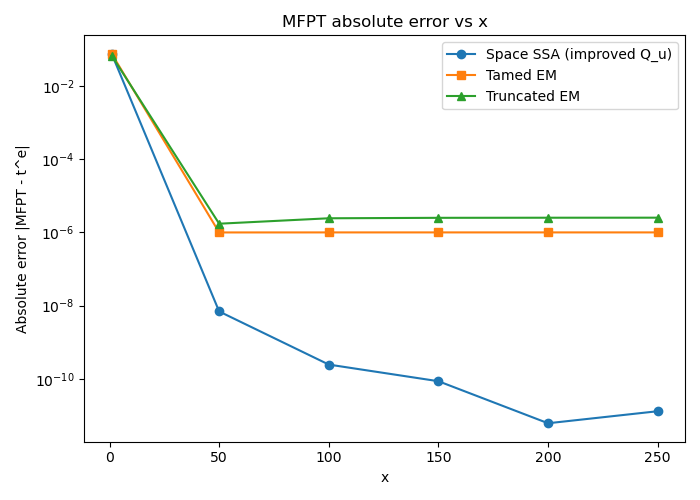
\includegraphics[width=0.45\textwidth]{fig/Absolute_error.png}
	}\quad
	\subfloat[时间离散误差与空间离散误差比值]{%
		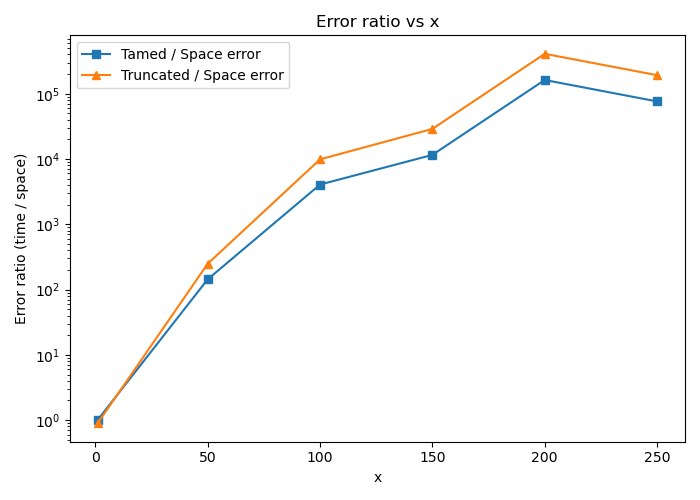
\includegraphics[width=0.45\textwidth]{fig/Error_ratio.png}
	}
	\caption{一维立方振子模型中，从 \(x\) 向左跨越固定距离 \(\delta\) 的平均时间误差比较：空间离散与时间离散的数值结果。}
	\label{fig:time-space-mfpt}
\end{figure}

从图~\ref{fig:time-space-mfpt}(a) 可以看到，在本节选取的参数范围内，随着初值 \(x\) 增大，三种方法得到的平均首达时间均快速趋近理论基准 \(t^e(x\to L)\)，这与前文的分析相符。其中，基于 \(Q_{u}\) 的 SSA 方法在大 \(x\) 区域的误差明显更小，数值上呈现出随 \(x\) 增大而迅速衰减的趋势，与 \(t^e\) 的主阶行为 \(\delta/x^3\) 一致，体现了空间离散在强漂移极限下对局部时间的良好刻度匹配。图~\ref{fig:time-space-mfpt}(b) 的误差比值进一步揭示：在较大的 \(x\) 下，时间离散方法的误差总体上显著大于空间离散误差，即
\[
R_{\mathrm{tame}}(x),\ R_{\mathrm{trunc}}(x) \gg 1,
\]
表明在同样的空间跨越距离和相近的计算代价下，基于生成元离散的 SSA 方法在该模型上能提供更稳定、更精确的时间估计。随着 \(x\) 增大，空间离散误差已降到非常小的量级，而时间离散误差逐渐受限于时间步长与蒙特卡罗方差，难以进一步降低，这也反映了在强漂移、长时间问题中，单纯减小时间步长未必比提高空间离散精度更划算。

综上，一维立方振子数值实验验证了前文关于在顺漂移和大初值情形下空间离散方法在固定空间跨越距离的时间估计方面具有明显优势的理论结论。

	\section{关于带退化噪声的随机系统的数值格式比较}
	\label{sec:langevin-invariant}
	
	本节以欠阻尼 Langevin 方程为对象，对基于生成元空间离散的混合（hybrid）格式与
	基于时间步进的 Euler--Maruyama（EM）格式在数值求解不变测度上的精度与计算代价进行系统比较。
	与前几节中以首达时间和 逃逸概率 为弱量指标不同，本节直接以平稳概率密度作为比较对象，
	从而在同一精度尺度下给出两类方法的定量评价。
	
	\subsection{模型与精确不变测度}
	
	考虑如下二维欠阻尼 Langevin 方程（又称动力学朗之万方程）：
	\begin{equation}\label{eq:langevin}
		\begin{cases}
			\mathrm{d}x_t = v_t\,\mathrm{d}t, \\
			\mathrm{d}v_t = \bigl(-x_t - \gamma v_t\bigr)\,\mathrm{d}t + \sigma\,\mathrm{d}W_t,
		\end{cases}
	\end{equation}
	其中 $(x_t, v_t)\in\mathbb{R}^2$，$x_t$ 为位移，$v_t$ 为速度，$\gamma>0$ 为阻尼系数，
	$\sigma>0$ 为噪声强度，$W_t$ 为一维标准布朗运动。
	方程 \eqref{eq:langevin} 对应的势函数为调和势 $U(x) = x^2/2$，其无穷小生成元为
	\begin{equation}\label{eq:langevin-gen}
		L = v\,\partial_x + (-x - \gamma v)\,\partial_v
		+ \frac{\sigma^2}{2}\,\partial_{vv}.
	\end{equation}
	系统满足涨落耗散定理，具有唯一的平稳（不变）概率密度
	\begin{equation}\label{eq:langevin-true}
		\rho^*(x, v)
		= \frac{\beta}{2\pi}\exp\!\Bigl(-\beta\,\frac{x^2 + v^2}{2}\Bigr),
		\qquad \beta = \frac{2\gamma}{\sigma^2},
	\end{equation}
	即不变测度为以原点为中心、协方差矩阵为 $\beta^{-1} I_2$ 的二维各向同性 Gauss 分布。
	该精确解为后续数值方法提供了可靠的参照基准。
	
	\subsection{空间离散格式：混合（hybrid）$\widetilde{Q}_u$ 方法}
	
	\subsubsection{离散生成元与转移矩阵的构造}
	
	对方程 \eqref{eq:langevin}，令 $(x_1, x_2) = (x, v)$，漂移向量为
	\[
	\mu(x, v) = \bigl(v,\ -x - \gamma v\bigr),
	\]
	扩散矩阵为
	\[
	M = \begin{pmatrix} 0 & 0 \\ 0 & \sigma^2/2 \end{pmatrix}.
	\]
	注意 $x$ 方向上扩散为零，$v$ 方向上扩散为 $M_{22} = \sigma^2/2$，
	这是典型的退化扩散结构。
	需要指出的是，方程 \eqref{eq:langevin} 的扩散仅作用于速度变量 $v$，
	而位置变量 $x$ 仅通过漂移项与 $v$ 耦合，因此该系统属于典型的退化噪声随机系统。
	尽管扩散矩阵是奇异的，但由于漂移与扩散之间存在耦合，
	系统仍具有良好的长时间统计性质，并存在唯一不变测度。
	这使其成为检验退化噪声情形下数值格式逼近平稳分布能力的一个标准模型。
	
	在计算域 $[-L_x, L_x]\times[-L_v, L_v]$ 上取均匀网格，步长分别为 $h_x$ 和 $h_v$，
	网格点记为 $(x_i, v_j)$，$i = 0, \dots, N_x$，$j = 0, \dots, N_v$。
	对每个内部格点，依照改进的有限差分格式 $\widetilde{Q}_u$（见 \eqref{algorithm:Q_u_tilde_rewrite}），
	各方向的跳跃率定义如下。
	
	在 $x$ 方向，漂移为 $\mu_x = v$，扩散为零，令
	\[
	q_{x+}(x_i, v_j) = \frac{v_j^+}{h_x},\qquad
	q_{x-}(x_i, v_j) = \frac{v_j^-}{h_x},
	\]
	其中 $a^+ = \max(a, 0)$，$a^- = \max(-a, 0)$。
	
	在 $v$ 方向，漂移为 $\mu_v = -x - \gamma v$，修正扩散系数为
	\[
	\widetilde{M}_{22}(x_i, v_j)
	= \frac{1}{2}\max\!\Bigl(\sigma^2 - \lvert\mu_v(x_i,v_j)\rvert\,h_v,\ 0\Bigr),
	\]
	跳跃率为
	\[
	q_{v+}(x_i, v_j)
	= \frac{\mu_v^+(x_i,v_j)}{h_v} + \frac{\widetilde{M}_{22}(x_i,v_j)}{h_v^2},\qquad
	q_{v-}(x_i, v_j)
	= \frac{\mu_v^-(x_i,v_j)}{h_v} + \frac{\widetilde{M}_{22}(x_i,v_j)}{h_v^2}.
	\]
	边界处采用截断处理，即令到达域外的跳跃率为零。
	
	由上述跳跃率构造的离散生成元 $Q_h$ 是一个稀疏的 $Q$-矩阵，
	其对应的连续时间马尔可夫链具有唯一平稳分布 $\pi^h$，满足
	\[
	\pi^h Q_h = 0,\qquad \sum_{(i,j)} \pi^h(x_i, v_j) = 1.
	\]
	将 $\pi^h$ 除以网格面积 $h_x h_v$ 即得到平稳密度的数值近似 $\rho^h(x_i, v_j)$。
	
%	\subsubsection{平稳分布的数值求解}
%	
%	求解平稳分布等价于求转移矩阵 $P = I + Q_h/\lambda$（其中 $\lambda$ 为均匀化参数）
%	的主左特征向量，即满足 $\pi P = \pi$ 的概率向量。
%	本节采用如下均匀化幂迭代方案（uniformization power iteration）：
%	
%	\begin{enumerate}
%		\item 计算各格点的总流出率 $\lambda_i = -q_{ii}$，取均匀化参数
%		$\lambda = 1.05\,\max_i\,\lambda_i + \varepsilon_0$（$\varepsilon_0 = 10^{-14}$）；
%		\item 构造均匀化转移矩阵 $P$，其中对角元 $P_{ii} = 1 - \lambda_i/\lambda$，
%		非对角元 $P_{ij} = q_{ij}/\lambda$（$j\ne i$）；
%		\item 以均匀初始分布 $p^{(0)} = \mathbf{1}/N$ 出发，
%		迭代 $p^{(k+1)} = P^\top p^{(k)}$，并在每步后归一化，
%		直至 $\|p^{(k+1)} - p^{(k)}\|_\infty < \varepsilon_{\mathrm{tol}}$（默认 $\varepsilon_{\mathrm{tol}} = 10^{-11}$）。
%	\end{enumerate}
%	
%	\noindent
%	矩阵 $P$ 以稀疏 CSR 格式存储，每个格点至多 5 个非零元（自身加四邻居），
%	稀疏矩阵向量乘法借助多线程 BLAS 库实现并行加速。
	
	\subsection{时间离散格式：Euler--Maruyama 方法}
	
	对方程 \eqref{eq:langevin} 应用标准 Euler--Maruyama（EM）格式，时间步长为 $\Delta t$，
	离散迭代为
	\begin{equation}\label{eq:langevin-EM}
		\begin{cases}
			x_{n+1} = x_n + v_n\,\Delta t, \\
			v_{n+1} = v_n + (-x_n - \gamma v_n)\,\Delta t + \sigma\,\sqrt{\Delta t}\,\xi_n,
		\end{cases}
	\end{equation}
	其中 $\{\xi_n\}$ 为独立同分布的标准正态随机变量。
	
	由于方程 \eqref{eq:langevin} 的漂移项关于 $(x, v)$ 为线性，且满足全局 Lipschitz 与线性增长条件，
	经典 Euler--Maruyama 格式在强意义下具有 $1/2$ 阶收敛，
	无需采用驯服或截断改进即可保证数值稳定性。
	
	根据遍历定理，对方程 \eqref{eq:langevin-EM} 产生的遍历 Markov 链，
	沿一条足够长的轨迹 $(x_0, v_0), (x_1, v_1), \dots, (x_M, v_M)$ 的时间平均收敛到空间平均：
	\[
	\frac{1}{M}\sum_{n=0}^{M-1} f(x_n, v_n)
	\xrightarrow{M\to\infty}
	\int f(x, v)\,\rho^*(x, v)\,\mathrm{d}x\,\mathrm{d}v.
	\]
	因此，以长轨迹的二维直方图作为不变密度的 EM 数值估计：
	对给定网格 $(x_i, v_j)$，统计轨迹落入各格点邻域的频率，
	再除以网格面积 $h_x h_v$ 即得密度估计 $\rho^{\mathrm{EM}}(x_i, v_j)$。
	
%	EM 方法的误差来源有两部分：
%	\begin{itemize}
%		\item \textbf{时间离散误差}：EM 格式对真实 SDE 的弱逼近阶为 $O(\Delta t)$，
%		步长 $\Delta t$ 越小，数值平稳分布对真实不变测度的偏差越小；
%		\item \textbf{统计误差}：有限轨迹长度带来的 Monte Carlo 方差，
%		与轨迹步数 $M$ 的关系为 $O(1/\sqrt{M})$，
%		该误差与网格剖分无关，决定了 EM 方法在固定时间窗内精度的上限。
%	\end{itemize}
	
	
	
	
	\subsection{二阶格式的推导}
	
	扩散过程的无穷小生成元（Infinitesimal generator）$L$ 定义如下：
	\begin{equation}
		Lf(x) = \mu(x) \cdot Df(x) + \frac{1}{2} \sigma \sigma^\top D^2 f(x)
	\end{equation}
	
	采用中心差分格式（Central difference scheme），我们定义离散算子 $Qf(x)$ 如下：
	\begin{equation}
		\begin{aligned}
			Qf(x) = & \sum_{i} \mu_i(x) \cdot \frac{f(x+he_i) - f(x-he_i)}{2h} \\
			& + \sum_{i} \frac{1}{2} \sigma_{ii}^2 \cdot \frac{f(x+he_i) + f(x-he_i) - 2f(x)}{h^2}
		\end{aligned}
	\end{equation}
	
	通过重新排列各项，并按增量 $[f(x \pm he_i) - f(x)]$ 进行归类，上述表达式可以改写为：
	\begin{equation}
		\begin{aligned}
			Qf(x) = & \sum_{i} \left( \frac{\mu_i(x)}{2h} + \frac{\sigma_{ii}^2}{2h^2} \right) \left[ f(x+he_i) - f(x) \right] \\
			& + \sum_{i} \left( -\frac{\mu_i(x)}{2h} + \frac{\sigma_{ii}^2}{2h^2} \right) \left[ f(x-he_i) - f(x) \right]
		\end{aligned}
	\end{equation}
	
	\vspace{1em}
	\noindent \textbf{关于漂移项分解（上风逻辑）的说明：} \\
	为了确保离散格式系数的稳定性（即保证跳跃速率的非负性），需要对漂移项 $\mu$ 进行如下分解：
	\begin{align}
		\frac{\mu}{2} &= \mu \vee 0 - \frac{|\mu|}{2} \\
		-\frac{\mu}{2} &= \mu \wedge 0 - \frac{|\mu|}{2}
	\end{align}
	
	进而得到 $Q_u^{LZ}$ 格式的表达式：
	\begin{equation}
		\begin{aligned}
			Q_u^{LZ} f(x) = & \sum_{i=1}^{n} \left( \frac{\mu_i(x) \vee 0}{h} + \frac{M_{ii}(x)}{h^2} \right) \left( f(x+he_i) - f(x) \right) \\
			& + \left( -\frac{\mu_i(x) \wedge 0}{h} + \frac{M_{ii}(x)}{h^2} \right) \left( f(x-he_i) - f(x) \right)
		\end{aligned}
	\end{equation}
	
	其中，$M_{ii}(x)$ 是为了修正扩散项而定义的修正系数：
	\begin{equation}
		M_{ii}(x) = 0.5 \times (\sigma_{ii}^2 - |\mu_i(x)|h) \vee 0
	\end{equation}
	
	
	\subsection{误差分析与数值实验结果}
	
	本小节将从理论一致性与数值实验两个维度，对混合 $\widetilde{Q}_u$ 格式与 Euler--Maruyama (EM) 格式在计算不变测度上的表现进行深入分析。
	
	
	\subsubsection{误差来源理论分析}
	
	对于不变测度的数值计算，两类方法的误差来源具有本质区别：
	
	\begin{enumerate}
		\item \textbf{EM 格式的弱误差与统计误差}：
		对方程 \eqref{eq:langevin-EM}，其离散过程产生的马尔可夫链的不变测度 $\rho_{\Delta t}$ 与连续系统精确测度 $\rho^*$ 之间的误差通常满足弱收敛阶：
		\[ \|\rho^* - \rho_{\Delta t}\| = O(\Delta t^k) \]
		对于标准 EM 格式，在计算不变测度时通常具有 $k=1$ 阶精度。此外，由于采用长轨迹时间平均进行估计，其总误差还受限于统计波动误差 $O(T^{-1/2})$，其中 $T$ 为模拟总时长。
		
		\item \textbf{Hybrid 格式的截断误差}：
		$\widetilde{Q}_u$ 格式的精度由离散生成元 $Q_h$ 对无穷小生成元 $L$ 的逼近程度决定。在 $v$ 方向，通过引入修正扩散项 $\widetilde{M}_{22}$，该格式在漂移项占优时退化为一阶上风格式，而在扩散项占优时接近二阶中心差分。在平稳分布求解中，其误差主要源于空间步长 $h = \max(h_x, h_v)$ 的幂次，通常表现为 $O(h)$ 至 $O(h^2)$ 之间的收敛阶。
	\end{enumerate}
	
	\subsubsection{EM 格式收敛阶测试}
	
	在实验中，固定参数 $\gamma=1, \sigma=1$，设置总时间 $T_{\text{total}} = 5 \times 10^5$，利用 $20$ 条独立轨迹进行并行采样。表 \ref{tab:em-error} 展示了不同时间步长 $\Delta t$ 下的 $L^1$ 误差。
	
	\begin{table}[htbp]
		\centering
		\caption{EM 格式在不同时间步长下的 $L^1$ 误差（$T=5\times 10^5$）}
		\label{tab:em-error}
		\begin{tabular}{cccc}
			\toprule
			步长 $\Delta t$ & $L^1$ 误差 & 局部收敛阶 & 计算耗时 (s) \\
			\midrule
			0.160 & $1.646\times 10^{-1}$ & — & 31.3 \\
			0.080 & $8.104\times 10^{-2}$ & 1.022 & 62.0 \\
			0.040 & $4.056\times 10^{-2}$ & 0.999 & 102.5 \\
			0.020 & $2.115\times 10^{-2}$ & 0.939 & 177.2 \\
			0.010 & $1.100\times 10^{-2}$ & 0.943 & 336.3 \\
			0.005 & $6.921\times 10^{-3}$ & 0.669 & 645.5 \\
			\bottomrule
		\end{tabular}
	\end{table}
	
	实验结果表明，当 $\Delta t \ge 0.01$ 时，EM 格式表现出稳定的 1 阶收敛。当步长减小至 $0.005$ 时，由于统计波动的量级逐渐接近离散截断误差，局部斜率出现下降，这说明单纯减小步长而不增加模拟时长已无法有效提升 EM 格式的精度。
	
	\subsubsection{Hybrid 格式收敛阶测试}
	
	针对同样的系统，采用混合 $\widetilde{Q}_u$ 格式，通过 ARPACK 特征值求解器计算离散生成元的主特征向量。实验取速度维网格数 $N_v \in [20, 80]$，位移维网格数对应取为 $N_x = N_v^2$ 以匹配退化方向的尺度。
	
	\begin{table}[htbp]
		\centering
		\caption{Hybrid $\widetilde{Q}_u$ 格式在不同空间步长下的 $L^1$ 误差}
		\label{tab:hybrid-error}
		\begin{tabular}{ccccc}
			\toprule
			网格数 $N_v$ & 步长 $h_v$ & $L^1$ 误差 & 局部收敛阶 & 计算耗时 (s) \\
			\midrule
			20 & 0.4211 & $4.81\times 10^{-2}$ & — & 11.51 \\
			40 & 0.2051 & $1.12\times 10^{-2}$ & 2.03 & 3.69 \\
			60 & 0.1356 & $4.87\times 10^{-3}$ & 2.02 & 26.95 \\
			80 & 0.1013 & $2.71\times 10^{-3}$ & 2.01 & 193.34 \\
			\bottomrule
		\end{tabular}
	\end{table}
	
	从表 \ref{tab:hybrid-error} 可以看出，Hybrid 格式在处理欠阻尼 Langevin 方程时展现出了优异的 \textbf{2 阶收敛特性}。值得注意的是，$N_v=20$ 时的耗时略高（11.51s），主要源于 Numba 库的首次实时编译（JIT）开销；随着计算规模增加，该方法展现了极高的计算效率。
	
	\subsubsection{综合评价与结论}
	
	图 \ref{fig:comparison-loglog} 汇总了两类方法的收敛曲线对比。
	
	% 此处插入 log-log 误差对比图
	% \begin{figure}[htbp]
		% 	\centering
		% 	\includegraphics[width=0.7\textwidth]{comparison_plot.png}
		% 	\caption{EM 格式与 Hybrid 格式的 $L^1$ 误差收敛阶对比}
		% 	\label{fig:comparison-loglog}
		% \end{figure}
	
	综合上述分析，可得出如下结论：
	\begin{itemize}
		\item \textbf{精度效率比}：Hybrid 格式在较低的网格密度下即可达到 EM 格式极长模拟时间才能获取的精度。对于低维退化随机系统，Hybrid 格式在计算不变测度上具有绝对优势。
		\item \textbf{统计稳定性}：Hybrid 格式作为一种确定性算法，避免了 EM 格式中由于随机采样带来的涨落，其结果具有极高的重现性。
		\item \textbf{适用范围}：EM 格式虽然在本例中效率较低，但其无需构造大型矩阵，在处理高维系统（$d \ge 4$）时仍是唯一可行的方案；而 Hybrid 格式则更适用于需要高精度密度分布图景的低维动力学分析。
	\end{itemize}
	
	
	
%============================================================
% 替换原论文中"随机 Canard 快-慢系统的动力学行为分析"一章
% 保留原有逃逸概率、CTRW方程等理论框架，
% 新增：噪声强度分析（sigma_c理论）+ CTMC格式与EM格式数值比较
% 图像命名与代码输出一致
% ============================================================

\section{Canard}

\subsection{模型与快慢分解}

考虑二维快慢系统（$\varepsilon=\delta\in(0,1)$ 很小）：
\begin{equation}\label{eq:model}
	\varepsilon \dot x = y - f(x),\qquad \dot y = a-x,
	\qquad f(x)=\frac{x^3}{3}-x .
\end{equation}

\subsection{快时间与层系统（layer problem）}
引入快时间 $\tau=t/\varepsilon$，记 $\frac{d}{d\tau}(\cdot)=(\cdot)'$，则
\begin{equation}\label{eq:layer}
	x' = y-f(x),\qquad y'=0 .
\end{equation}
因此在快时间尺度上 $y$ 可视为参数；$x$ 很快被吸引/排斥到快子系统的平衡点集合。

\subsection{临界流形（critical manifold）与稳定性}
层系统平衡点满足 $y=f(x)$，得到临界流形
\begin{equation}\label{eq:C0}
	\mathcal C_0=\{(x,y): y=f(x)\}.
\end{equation}
线性化：$\partial_x(y-f(x)) = -f'(x)=-(x^2-1)$。
因此
\[
|x|>1\Rightarrow f'(x)>0 \Rightarrow \partial_x(y-f(x))<0 \ \text{（吸引支）},\qquad
|x|<1\Rightarrow \partial_x(y-f(x))>0 \ \text{（排斥支）}.
\]
折点（saddle--node/ fold）由 $f'(x)=0$ 给出：
\begin{equation}\label{eq:folds}
	x=\pm 1,\qquad y=f(\pm 1)=\mp\frac{2}{3}.
\end{equation}

\subsection{慢系统（reduced problem）与 Fenichel 慢流形}

\subsection{慢极限（$\varepsilon\to0$）上的约化方程}
在慢时间 $t$ 下，令 $\varepsilon=0$，得到代数约束 $y=f(x)$，并且
\[
\dot y = f'(x)\dot x.
\]
由 $\dot y=a-x$ 得到约化慢方程（在 $\mathcal C_0$ 上）：
\begin{equation}\label{eq:reduced}
	\dot x = \frac{a-x}{f'(x)}=\frac{a-x}{x^2-1},
	\qquad y=f(x).
\end{equation}
注意在折点 $x=\pm1$ 处分母为 $0$，意味着慢流在折点处“失效”，轨道会发生快跳。

\subsection{Fenichel 理论给出的 $\mathcal C_\varepsilon^{a/r}$}
当 $\varepsilon>0$ 足够小，远离折点的吸引支与排斥支会分别扰动为
\[
\mathcal C_\varepsilon^{a},\ \mathcal C_\varepsilon^{r},
\]
并保持与 $\mathcal C_0$ 同胚（光滑）且具有指数吸引/排斥性质（这就是 Canard 理论的几何骨架）。
（Sowers 用一般三次型 $f$ 将 $\mathcal C_0$ 分成稳定支 $S_L,S_R$ 与不稳定支 $U$：稳定与不稳定的划分思想与此一致。）%
% 资料来源（一般三次型的慢流形分支划分）：:contentReference[oaicite:0]{index=0}

\subsection{确定性动力学：平衡点、松弛振荡、鸭解（regular duck / headless duck）}

\subsection{平衡点与线性稳定性}
由 \eqref{eq:model} 得平衡点
\[
x^\ast=a,\qquad y^\ast=f(a)=\frac{a^3}{3}-a.
\]
Jacobi 矩阵为
\[
J=
\begin{pmatrix}
	\frac{1}{\varepsilon}(1-a^2) & \frac{1}{\varepsilon}\\[3pt]
	-1 & 0
\end{pmatrix},
\quad
\mathrm{tr}(J)=\frac{1-a^2}{\varepsilon},\quad
\det(J)=\frac{1}{\varepsilon}>0.
\]
故当 $|a|>1$ 时 $\mathrm{tr}(J)<0$，平衡点稳定；当 $|a|<1$ 时平衡点不稳定。
特别地，$a=\pm1$ 是临界（“Hopf 型临界”）位置，并且在本快慢问题中它恰好与折点重合（$a=1$ 对应 $(1,-2/3)$，$a=-1$ 对应 $(-1,2/3)$），这正是 Canard 爆炸发生的典型几何情形。

\subsection{为什么会出现松弛振荡（relaxation oscillation）？}
当 $|a|<1$ 时，平衡点落在排斥区（因为 $|x^\ast|=|a|<1$），轨道不能收敛到平衡点。
在 $\varepsilon\ll1$ 时，典型轨道呈现“两段慢爬 + 两次快跳”的结构：

\begin{itemize}
	\item 在吸引慢流形 $\mathcal C_\varepsilon^{a}$ 上按 \eqref{eq:reduced} 慢慢移动；
	\item 接近折点 $x=1$（或 $x=-1$）时，吸引慢流形终止，轨道在快时间尺度上沿层系统 \eqref{eq:layer} 快速跳到另一条吸引支附近；
	\item 重复上述过程形成闭合周期轨道（松弛振荡）。
\end{itemize}

\paragraph{奇异极限下的“跳跃落点”可以显式写出。}
例如到达右折点 $(1,-2/3)$ 时，$y$ 近似保持 $y=-2/3$ 不变，快方程把 $x$ 拉到 $y=f(x)$ 的稳定根。
解 $f(x)=-2/3$：
\[
\frac{x^3}{3}-x=-\frac{2}{3}
\iff x^3-3x+2=0
\iff (x-1)^2(x+2)=0.
\]
因此从 $x=1$ 会快跳到另一稳定根 $x=-2$（而不是停留在重根 $x=1$）。
同理，在左折点 $(-1,2/3)$ 处解 $f(x)=2/3$：
\[
x^3-3x-2=0 \iff (x+1)^2(x-2)=0,
\]
故从 $x=-1$ 会快跳到 $x=2$。

\paragraph{周期的慢段可由积分近似。}
在右吸引支上 $x$ 从 $2$ 慢走到 $1$；在左吸引支上 $x$ 从 $-2$ 慢走到 $-1$。
由 \eqref{eq:reduced} 得慢段时间近似
\begin{equation}\label{eq:period}
	T \approx \int_{1}^{2}\frac{x^2-1}{x-a}\,dx \;+\; \int_{-2}^{-1}\frac{x^2-1}{a-x}\,dx,
	\qquad (|a|<1,\ \varepsilon\ll1).
\end{equation}
这体现了松弛振荡的“长时间慢漂移 + 短时间快跳”。

\subsection{为什么会出现 regular duck 与 headless duck？（Canard 几何机制）}

\paragraph{核心几何：排斥慢流形附近的“指数放大”。}
当参数 $a$ 接近临界值（尤其在 $a\approx 1$ 且 $\varepsilon\ll1$）时，轨道可能在排斥慢流形 $\mathcal C_\varepsilon^{r}$ 附近停留一段时间。
在排斥支上，快方向的线性化增长率约为
\[
\dot \xi \approx \frac{1}{\varepsilon}(1-x^2)\,\xi,
\]
而在 $|x|<1$ 时 $1-x^2>0$，因此任何微小偏差 $\xi$ 会以 $e^{c/\varepsilon}$ 的量级被放大。
这导致一个著名现象：$a$ 只需发生极微小（常常是指数小窗口）的变化，周期轨道的幅值就会从“小振幅”突然跃迁到“松弛大振幅”（Canard explosion）。

\paragraph{regular duck vs headless duck（用“跳回哪条稳定支”区分）。}
沿排斥支走一段后，轨道终究会“跑不动”并从排斥区脱离，回到某条吸引支。
如果它回到左吸引支，就得到 \textbf{regular duck}；若回到右吸引支，就得到 \textbf{headless duck}。
Sowers 在一般三次型快慢系统中用图像语言明确指出：轨道在排斥慢流形 $U$ 上“绕行”后，最终回到稳定慢流形 $S$；
回到 $S_L$ 是 regular duck，回到 $S_R$ 是 headless duck。%
% 资料来源（regular/headless 的定义性描述）：:contentReference[oaicite:1]{index=1}

\paragraph{与参数 $a,\varepsilon$ 的关系（定性结论）。}
\begin{itemize}
	\item 当 $|a|>1$：平衡点稳定，轨道通常收敛到平衡点（不振荡）。
	\item 当 $|a|<1$ 且远离临界：存在稳定松弛振荡（大振幅）。
	\item 当 $a$ 位于靠近 $1$（或 $-1$）的极窄窗口：出现 Canard 轨道；
	窗口内随 $a$ 变化会出现 headless duck $\leftrightarrow$ regular duck $\leftrightarrow$ relaxation oscillation 的快速切换（Canard 爆炸）。
\end{itemize}

\paragraph{（可用于写作的具体参数展开）}
经典 van der Pol/Canard 理论给出“canard 点”参数 $a=a_c(\varepsilon)$ 的渐近展开（你的代码里使用过）：
\[
a_c(\varepsilon)=1-\frac{\varepsilon}{8}-\frac{3\varepsilon^2}{32}-\frac{173\varepsilon^3}{1024}+\cdots,
\]
在 $a$ 穿过 $a_c(\varepsilon)$ 的极窄区间时，轨道从 headless 转向 regular，并迅速爆炸到松弛振荡。
（该展开的严格推导通常用 blow-up/匹配渐近或正则形化方法完成，见参考文献中的 Krupa--Szmolyan 等。）

\subsection{加入噪声后的 Canard：慢变量噪声 $\Rightarrow$ 随机选择；快变量噪声 $\Rightarrow$ 随机共振}

\subsection{两种加噪方式}
对 \eqref{eq:model} 常见的两种加性白噪声版本为：

\paragraph{(A) 噪声加在慢变量（$y$）上：}
\begin{equation}\label{eq:slow-noise}
	dx_t=\frac{1}{\varepsilon}\bigl(y_t-f(x_t)\bigr)\,dt,\qquad
	dy_t=(a-x_t)\,dt+\sigma\,dW_t .
\end{equation}

\paragraph{(B) 噪声加在快变量（$x$）上：}
\begin{equation}\label{eq:fast-noise}
	dx_t=\frac{1}{\varepsilon}\bigl(y_t-f(x_t)\bigr)\,dt+\frac{\sigma}{\varepsilon}\,dW_t,\qquad
	dy_t=(a-x_t)\,dt .
\end{equation}

Sowers 明确说明：本文主要研究噪声进入慢变量时导致“regular vs headless”的\textbf{随机选择}；
而把噪声放进快变量会出现\textbf{随机共振}等不同现象，并引用相关工作。%
% 资料来源（慢变量噪声导致随机选择的研究目标；快变量噪声可致随机共振的说明）：:contentReference[oaicite:2]{index=2}:contentReference[oaicite:3]{index=3}

\subsection{慢变量噪声为什么会导致“随机选择”？（数学机制）}

\subsubsection{机制 1：排斥慢流形上的指数放大把噪声“放大成选择”}
在 canard 瓶颈区域，轨道必须贴着排斥慢流形 $\mathcal C_\varepsilon^{r}$ 走一段。
设与排斥慢流形的快向偏差为 $\xi$，其主导项满足（见上一节）
\[
\dot \xi \approx \frac{\lambda(t)}{\varepsilon}\xi,\qquad \lambda(t)>0.
\]
因此任何由噪声引入的、哪怕极微小的随机偏差，在时间推进中都会被放大为 $O(1)$ 的差异，
从而决定轨道最终回到哪条吸引支（$S_L$ 或 $S_R$），即决定 \textbf{regular duck 或 headless duck}。
这就是“随机选择”的本质：\textbf{确定性系统中由参数决定的极其敏感的分界，被噪声模糊成概率分界。}

\subsubsection{机制 2：Sowers 的极限定理——分界量的符号趋于高斯分布}
Sowers 构造了刻画“靠近慢流形时偏离量”的量 $D_\varepsilon(\cdot)$，
并在合适缩放下证明它的极限分布含有高斯项，因而轨道以某个概率趋向 $+\infty$ 或 $-\infty$，
对应“落到左支/右支”的随机选择概率（高斯分布函数 $\Phi$ 给出）。
例如在其结论之一中，极限概率写成 $\int_{-\infty}^{m} e^{-z^2/2}dz$ 的形式。%
% 资料来源（极限分布含高斯项，从而得到趋向 ±∞ 的概率公式）：:contentReference[oaicite:4]{index=4}
这正是“随机选择（random decision/selection）”的严格概率论版本：\textbf{在 canard 分界附近，轨道去 regular 或 headless 不再由参数单独决定，而是由噪声驱动的随机变量决定。}

\subsubsection{机制 3：折点附近的局部正则形（Berglund--Gentz 的样本路径推导）}
Berglund--Gentz 在 van der Pol 型系统中研究了\emph{慢变量加噪}：
\begin{equation}\label{eq:BG-619}
	dx_t=\frac{1}{\varepsilon}\Bigl(y_t+x_t-\frac{x_t^3}{3}\Bigr)dt,\qquad
	dy_t=-x_t\,dt+\sigma\,dW_t .
\end{equation}
% 资料来源（式 (6.1.19)）：:contentReference[oaicite:5]{index=5}

它的关键动力学发生在折点（鞍结分岔点）附近。以右折点 $(x_c,y_c)=(1,-2/3)$ 为例，
作局部变换（其符号选择使正则形更标准）：
\[
(\tilde x_t,\tilde y_t)=(x_t-x_c,\; -(y_t-y_c)).
\]
在折点邻域可化为正则形的小扰动：
\begin{equation}\label{eq:BG-620}
	d\tilde x_t=\frac{1}{\varepsilon}\bigl(-\tilde y_t-\tilde x_t^2\bigr)\,dt,\qquad
	d\tilde y_t=dt+\sigma\,dW_t .
\end{equation}
% 资料来源（式 (6.1.20)）：:contentReference[oaicite:6]{index=6}

\paragraph{“贴慢流形的绝热解”与偏差方程。}
确定性情形 $\sigma=0$ 存在绝热解 $\bar x(\tilde y,\varepsilon)$ 追踪慢流形 $x^\ast(y)=|y|^{1/2}$，
并且当 $\tilde y\lesssim -\varepsilon^{2/3}$ 时偏离量随 $|\tilde y|$ 变化具有可控估计。
定义噪声诱导偏差
\[
\xi_t=\tilde x_t-\bar x(\tilde y_t,\varepsilon),
\]
则其满足（含漂移、非线性项与有效噪声强度）：
\begin{equation}\label{eq:BG-621}
	d\xi_t=\frac{1}{\varepsilon}\Bigl(a(\tilde y_t)\xi_t-\xi_t^2-\frac{1}{2}\sigma^2\varepsilon\,\partial_{yy}\bar x(\tilde y_t,\varepsilon)\Bigr)\,dt
	+\sigma\,g(\tilde y_t)\,dW_t,
\end{equation}
其中
\begin{equation}\label{eq:BG-622-623}
	a(y)=-2\bar x(y,\varepsilon),\qquad g(y)=-\partial_y\bar x(y,\varepsilon).
\end{equation}
并且在 $y\lesssim -\varepsilon^{2/3}$ 时
\[
a(y)\sim -|y|^{1/2},\qquad g(y)\sim |y|^{-1/2}.
\]
% 资料来源（式 (6.1.21)--(6.1.23) 及渐近行为）：:contentReference[oaicite:7]{index=7}

\paragraph{线性近似下的方差增长：解释“为何折点附近噪声影响被放大”。}
取线性近似
\begin{equation}\label{eq:BG-624}
	d\xi^{0}_t=\frac{1}{\varepsilon}a(\tilde y^{\mathrm{det}}_t)\xi^{0}_t\,dt+\sigma\,g(\tilde y^{\mathrm{det}}_t)\,dW_t,
\end{equation}
其方差增长满足
\[
\mathrm{Var}(\xi^{0}_t)\sim \frac{\sigma^2\varepsilon}{|\tilde y^{\mathrm{det}}_t|^{3/2}},
\qquad
\text{典型扩散尺度 }\ |\xi|\sim \frac{\sigma\,\varepsilon^{1/2}}{|\tilde y|^{3/4}}.
\]
% 资料来源（方差与典型扩散尺度）：:contentReference[oaicite:8]{index=8}

这条公式直接告诉你：当轨道慢慢接近折点（$|\tilde y|\to0$）时，
即使 $\sigma$ 固定不大，快方向的随机扩散尺度也会被 $|\tilde y|^{-3/4}$ 放大，
从而更容易触发“提前/延后跳跃”以及在 canard 分界附近的“落左/落右”的随机选择。

\paragraph{与“regular/headless”的连接（写作建议）。}
在 canard 窗口内，确定性系统中“落左/落右”对参数 $a$ 极端敏感；
而 \eqref{eq:BG-624} 的扩散放大意味着：在折点/排斥段附近，轨道会获得一个
近似高斯的横向随机偏移，随后又被排斥动力学指数放大，
最终把“横向偏移的符号/大小”转化成“落到 $S_L$ 或 $S_R$ 的概率”——这正是随机选择的数学机制。

\subsection{快变量噪声为什么会导致“随机共振（stochastic resonance）”？（数学机制）}

\subsubsection{随机共振的标准定义（与快慢系统的对应）}
随机共振通常指：系统在\textbf{弱周期信号}（或慢调制）作用下，本来难以跨越阈值/势垒发生切换；
加入\textbf{适当强度}的噪声后，切换事件与周期信号产生最强同步，导致输出的信号-噪声比或谱峰在某个噪声强度处达到最大。

在快慢系统中，慢变量（或慢流形几何）往往提供一个缓慢变化的“势垒高度/阈值位置”；
而当噪声直接作用于快变量时，快变量在短时间内被噪声“踢过”分界（例如跨过不稳定支或在折点前提前跳跃），
于是产生与慢调制相关的“近周期切换”。当噪声太小，几乎不切换；噪声太大，切换太随机；
中间某个噪声强度使平均切换时间与慢时间尺度（或外加周期）匹配，从而出现“共振”。

\subsubsection{用 Kramers 型速率解释“为何存在最优噪声强度”}
在许多等效一维阈值/势垒模型中，跨越事件的速率可近似为
\[
r(t)\approx C(t)\exp\Bigl(-\frac{\Delta V(t)}{\sigma^2}\Bigr),
\]
其中 $\Delta V(t)$ 随慢变量缓慢变化（慢变量相当于对势垒做慢调制）。
当慢调制有特征周期 $T_{\mathrm{slow}}$（例如松弛振荡或外部微弱周期输入），
随机共振常对应
\[
\mathbb E[\tau_{\mathrm{switch}}]\approx \frac{T_{\mathrm{slow}}}{2}
\quad\Longleftrightarrow\quad
r(\sigma)\approx \frac{2}{T_{\mathrm{slow}}},
\]
从而在某个 $\sigma$ 处同步最强、谱峰最明显。

\subsubsection{与 Canard/van der Pol 几何的直接对应}
对 \eqref{eq:fast-noise}，噪声项在 $x$ 方程中被 $1/\varepsilon$ 放大（若仍用加性白噪写法），
这意味着快方向的随机扰动会更直接、更强烈地影响“何时离开吸引支、何时跨过不稳定区”，
从而把“慢变量的缓慢变化”转化为“随机切换事件的相位锁定”。
因此快变量噪声下更典型地观察到随机共振/相干共振等现象，而不是像慢变量噪声那样主要表现为
“regular vs headless 的随机选择”。
（Sowers 也指出：把噪声放入快变量会导致随机共振等不同现象，并引相关文献。）%
% 资料来源（快变量噪声可致随机共振的说明）：:contentReference[oaicite:9]{index=9}

\subsection{在快变量和慢变量上分别加噪声}


\begin{enumerate}
	\item \textbf{模型层}：写出慢变量加噪的 van der Pol SDE \eqref{eq:BG-619}，并强调“关键发生在折点”。%
	% 资料来源：式 (6.1.19) 与折点重要性叙述:contentReference[oaicite:10]{index=10}
	\item \textbf{局部正则形层}：给出折点邻域正则形 \eqref{eq:BG-620}，指出它是鞍结正则形的随机扰动。%
	% 资料来源：式 (6.1.20):contentReference[oaicite:11]{index=11}
	\item \textbf{样本路径估计层}：给出偏差 SDE \eqref{eq:BG-621}--\eqref{eq:BG-624} 与方差/扩散尺度结论，
	用 $|\tilde y|^{-3/4}$ 的放大量解释“为什么接近折点时噪声效果突然变强”，再把它与 canard 分界的指数敏感性结合，
	得到“随机选择”的机制闭环。%
	% 资料来源：式 (6.1.21)--(6.1.24) 与方差结论:contentReference[oaicite:12]{index=12}
\end{enumerate}


%
%\begin{thebibliography}{99}
%	
%	\bibitem{Sowers2008}
%	R.\ B.\ Sowers,
%	\newblock \textit{Random Perturbations of Canards},
%	\newblock Journal of Theoretical Probability, 21 (2008), 824--889.
%	% 你上传的 PDF：Random Perturbations of Canards.pdf
%	% 相关出处：随机选择（摘要）:contentReference[oaicite:13]{index=13}；regular/headless 定义:contentReference[oaicite:14]{index=14}；
%	% 快变量噪声与随机共振提示:contentReference[oaicite:15]{index=15}。
%	
%	\bibitem{BerglundGentzBook}
%	N.\ Berglund and B.\ Gentz,
%	\newblock \textit{Noise-Induced Phenomena in Slow-Fast Dynamical Systems: A Sample-Paths Approach},
%	\newblock Springer, 2006.
%	% 你上传的 4 页摘录：式 (6.1.19)--(6.1.24) 与方差结论:contentReference[oaicite:16]{index=16}。
%	
%	\bibitem{Benoit1981}
%	E.\ Beno\^{\i}t, J.-L.\ Callot, F.\ Diener, and M.\ Diener,
%	\newblock \textit{Chasse au canard},
%	\newblock Collectanea Mathematica, 32 (1981), 37--119.
%	% Canard 经典起源文献。
%	
%	\bibitem{KrupaSzmolyan}
%	M.\ Krupa and P.\ Szmolyan,
%	\newblock \textit{Extending Geometric Singular Perturbation Theory to Nonhyperbolic Points---Fold and Canard Points},
%	\newblock (系列论文，2001--2004 年间多篇；用于 canard 点展开与严格几何证明).
%	
%	\bibitem{Gammaitoni1998}
%	L.\ Gammaitoni, P.\ H\"anggi, P.\ Jung, and F.\ Marchesoni,
%	\newblock \textit{Stochastic Resonance},
%	\newblock Reviews of Modern Physics, 70 (1998), 223--287.
%	% 随机共振综述（给出标准定义、Kramers 速率解释与 SNR 最优噪声强度思想）。
%	
%\end{thebibliography}

\section{随机 Canard 快-慢系统的动力学行为分析}
\label{sec:canard-dynamics}

\subsection{随机 Canard 系统与逃逸概率}

对于随机微分方程~\eqref{eq:SDE}，给定两个互不相交的 Borel 集 $A,B\subset D$，
定义首次到达时间
\[
\tau_A := \inf\{t\ge0 : X_t\in A\},\qquad
\tau_B := \inf\{t\ge0 : X_t\in B\}.
\]
逃逸概率函数定义为
\[
q(x) := \mathbb{P}_x\bigl(\tau_B < \tau_A\bigr),\qquad x\in D.
\]
经典结果表明 $q$ 满足如下椭圆型边值问题\cite{EV_TPT,EV_TowardsTP}：
\begin{equation}\label{eq:committor_PDE_ch4}
	\begin{cases}
		L q(x) = 0, & x\in D\setminus(A\cup B),\\[1mm]
		q(x) = 0, & x\in A,\\[1mm]
		q(x) = 1, & x\in B.
	\end{cases}
\end{equation}

本章考察如下二维快--慢随机 Canard 系统：
\begin{equation}\label{eq:canard-SDE-ch4}
	\begin{cases}
		\varepsilon\,\mathrm{d}x_t
		= \bigl(y_t - \tfrac{x_t^3}{3} + x_t\bigr)\,\mathrm{d}t,\\[4pt]
		\mathrm{d}y_t
		= (a - x_t)\,\mathrm{d}t + \sigma\,\mathrm{d}W_t,
	\end{cases}
\end{equation}
其中 $0<\varepsilon\ll1$ 为快--慢时间尺度比，$x_t$ 为快变量（无直接噪声），
$y_t$ 为慢变量（带加性噪声强度 $\sigma$），参数 $a$ 取特定值使系统出现
Canard 过渡，具体取为
\begin{equation}\label{eq:a-def}
	a = 1 - \frac{\varepsilon}{8} - \frac{3\varepsilon^2}{32}
	- \frac{173\varepsilon^3}{1024} - 0.01.
\end{equation}
系统的慢流形（$x$ 方程右端为零的零流形）为 $y = x^3/3 - x$，
鞍结点位于 $(x,y)=(1,-2/3)$。

\subsection{噪声强度与 Canard 现象的临界标度}
\label{subsec:noise-sigma-c}

\subsubsection{理论背景}

经典结果（Berglund--Gentz \cite{berglund2006noise}，第 6.1 节）给出了
随机 Canard 系统在鞍结点附近的局部标准形
\begin{equation}\label{eq:normal-form}
	\varepsilon\,\mathrm{d}\tilde x_t
	= (-\tilde y_t - \tilde x_t^2)\,\mathrm{d}t,\qquad
	\mathrm{d}\tilde y_t = \mathrm{d}t + \sigma\,\mathrm{d}W_t.
\end{equation}
在该标准形下，确定性 Canard 轨道沿慢流形 $\tilde x^\star(\tilde y)
= -|\tilde y|^{1/2}$（$\tilde y\leq 0$）跟踪。
设扰动 $\xi_t = \tilde x_t - \tilde x^\star(\tilde y_t,\varepsilon)$，则
其方差满足
\begin{equation}\label{eq:xi-variance}
	\mathrm{Var}(\xi_t) \sim
	\frac{\sigma^2\varepsilon}{|\tilde y_t|^{3/2}},
\end{equation}
即路径在 $x$ 方向的散布正比于 $\sigma\varepsilon^{1/2}/|\tilde y|^{3/4}$。

由此可以刻画出一个\textbf{临界噪声强度}
\begin{equation}\label{eq:sigma-c}
	\sigma_c = \varepsilon^{1/3}.
\end{equation}
具体地，Berglund--Gentz 证明了以下两种情形：
\begin{itemize}
	\item 若 $\sigma < \varepsilon^{1/3}$，路径在分岔点附近的最大散布为 $O(\sigma)$，
	小于稳定与不稳定绝热解之间的距离 $O(\varepsilon^{1/3})$，
	因此\textbf{样本路径在经过分岔点之前不大可能提前跳到另一支慢流形}，
	Canard 现象得以保持（图~\ref{fig:canard_ssa_vs_em}(a) 的上方部分）。
	\item 若 $\sigma > \varepsilon^{1/3}$，路径的典型散布达到稳定与不稳定绝热解
	之间距离的量级，\textbf{在 $\tilde y_t \sim -\sigma^{4/5}\varepsilon^{2/5}$
		处就可能提前转移到另一支慢流形}，Canard 结构被破坏
	（图~\ref{fig:canard_ssa_vs_em}(a) 的下方部分）。
\end{itemize}
因此 $\sigma_c = \varepsilon^{1/3}$ 构成 Canard 现象是否在噪声扰动下得以保持
的临界阈值。

\subsubsection{全局系统中的可观测量}

在全局 van der Pol 系统~\eqref{eq:canard-SDE-ch4} 中，上述局部理论
可通过以下可观测量在数值上加以验证。

\paragraph{跳变位置分布}
定义 $y_\mathrm{jump}$ 为路径首次穿越 $x=1$（鞍结点处）时对应的 $y$ 值。
确定性轨道满足 $y_\mathrm{det} \approx -0.77$（该值依赖 $\varepsilon$，
略低于鞍结点 $y_c = -2/3$）。当 $\sigma < \sigma_c$ 时，路径沿慢流形
充分跟踪，$y_\mathrm{jump}$ 集中在 $y_\mathrm{det}$ 附近，
标准差较小；当 $\sigma > \sigma_c$ 时，路径提前离开慢流形，
$\mathrm{std}(y_\mathrm{jump})$ 显著增大。

\paragraph{慢流形邻域停留时间}
定义路径在慢流形管道 $\{|x - x^\star(y)| \leq \delta_\mathrm{hit}\}$
内的时间占比（occupancy）为 Canard 质量的全局度量。

\paragraph{到达窗口的命中概率 $P_\mathrm{hit}$}
在慢流形上设定参考窗口
\begin{equation}\label{eq:window-A}
	A = \bigl\{(x,y):\; |y - y_\mathrm{ref}|\leq\eta,\;
	|x - x^\star(y)|\leq\delta_\mathrm{hit}\bigr\},
\end{equation}
其中 $y_\mathrm{ref}$ 靠近鞍结点但仍在正值稳定支上，统计路径在穿越
$x=1$ 之前进入 $A$ 的概率 $P_\mathrm{hit}$。
理论预测：$\sigma < \sigma_c$ 时 $P_\mathrm{hit}$ 接近 1，
$\sigma > \sigma_c$ 时 $P_\mathrm{hit}$ 显著下降。

\subsubsection{数值验证：$y_\mathrm{jump}$ 与 $\sigma$ 的关系}

取 $\varepsilon = 0.1$，$\sigma_c = \varepsilon^{1/3} \approx 0.464$，
起点 $(x_0, y_0) = (1.5,\, x_0^3/3 - x_0)$（位于正值稳定支上）。
对 $\sigma/\sigma_c \in [0.1, 2.0]$ 扫描，每组跑 $N=800$ 条路径，
用 EM 精细格式（$\Delta t = \varepsilon/100$）作为参考。

图~\ref{fig:canard_ssa_vs_em} 展示了四项统计量随 $\sigma/\sigma_c$ 的变化：

%\begin{figure}[!htbp]
%	\centering
%	
\includegraphics[width=\textwidth]{fig/canard_ssa_vs_em.png}
%	\caption{随机 Canard 系统四项统计量随噪声强度 $\sigma/\sigma_c$ 的变化
%		（$\varepsilon=0.1$，$\sigma_c = \varepsilon^{1/3} \approx 0.464$）。
%		竖虚线标记临界值 $\sigma = \sigma_c$。
%		(a) $P_\mathrm{hit}$：命中参考窗口 $A$ 的概率；
%		(b) 提前逃离概率 $P_\mathrm{esc}$；
%		(c) std$(y_\mathrm{jump})$；
%		(d) 离散化误差随步长/网格尺寸的收敛性（参考 EM 最精细解）。}
%	\label{fig:canard_ssa_vs_em}
%\end{figure}

从图~\ref{fig:canard_ssa_vs_em} 可以观察到：

\begin{enumerate}
	\item \textbf{临界行为的数值体现}：
	$P_\mathrm{hit}$（子图 (a)）在 $\sigma < \sigma_c$ 时保持高位，
	在 $\sigma \approx \sigma_c$ 附近开始明显下降；
	提前逃离概率 $P_\mathrm{esc}$（子图 (b)）在 $\sigma > \sigma_c$
	后显著上升，与理论一致。
	
	\item \textbf{跳变位置散布增大}：
	std$(y_\mathrm{jump})$（子图 (c)）在 $\sigma$ 增大时单调增大，
	$\sigma > \sigma_c$ 后增速明显加快，反映路径越来越早地离开慢流形。
	
	\item \textbf{EM 步长对 Canard 结构的敏感性}：
	子图 (d) 显示，当 $\Delta t \geq \varepsilon$ 时，EM 格式的离散化
	误差出现相变式跳跃，说明大步长 EM 会人为地"破坏"Canard 现象，
	而 CTMC（SSA）格式的误差随 $h_y$ 变化相对温和。
\end{enumerate}

\subsection{CTMC 格式的跳跃速率构造}
\label{subsec:jump-rates}

对于系统~\eqref{eq:canard-SDE-ch4}，采用 Chang--Cooper 混合格式
在二维网格上构造跳跃速率。取 $x$ 方向步长 $h_x$，$y$ 方向步长 $h_y$，
在格点 $(x_i, y_j)$ 处定义漂移
\[
\mu_x = \frac{y_j - x_i^3/3 + x_i}{\varepsilon},\qquad
\mu_y = a - x_i.
\]
$y$ 方向的混合项为
\begin{equation}\label{eq:m-y}
	m_y = \frac{1}{2}\max\!\bigl(\sigma^2 - |\mu_y|\,h_y,\;0\bigr),
\end{equation}
而 $x$ 方向无物理扩散，故 $m_x = 0$。四个方向的跳跃速率为
\begin{equation}\label{eq:jump-rates}
	\begin{aligned}
		q_{x+} &= \frac{\max(\mu_x,0)}{h_x},&\quad
		q_{x-} &= \frac{\max(-\mu_x,0)}{h_x},\\
		q_{y+} &= \frac{\max(\mu_y,0)}{h_y} + \frac{m_y}{h_y^2},&\quad
		q_{y-} &= \frac{\max(-\mu_y,0)}{h_y} + \frac{m_y}{h_y^2}.
	\end{aligned}
\end{equation}

\subsubsection{非均匀网格设计：$n_x = n_y^2$}

快变量 $x$ 方向无物理扩散，迎风格式引入的数值扩散为
\[
\text{数值扩散}_x \sim \frac{|\mu_x|\,h_x}{2}
= \frac{h_x}{2\varepsilon},
\]
在 $\varepsilon \ll 1$ 时即便 $h_x$ 适中，数值扩散也会远超物理量级。
为抑制此误差，令 $x$ 方向格点数为 $n_x = n_y^2$，从而
$h_x = h_y^2/c$ 量级，使数值扩散降至 $O(h_y^2/\varepsilon)$，
与 $y$ 方向的物理误差 $O(h_y)$ 相匹配。

以 $n_y = 60$（$h_y \approx 0.10$）为例，三种方案的比较如下：
\begin{table}[!htbp]
	\centering
	\caption{不同网格方案下数值扩散的比较（$\varepsilon=0.1$，$\sigma^2=2$，$n_y=60$）}
	\label{tab:grid-schemes}
	\begin{tabular}{lccccc}
		\toprule
		方案 & $n_x$ & $n_y$ & $h_x$ & $h_y$ & 数值扩散$_x \approx h_x/(2\varepsilon)$ \\
		\midrule
		均匀网格（原始） & 60 & 60 & $0.100$ & $0.100$ & $0.500$ \\
		本文方案 $n_x=n_y^2$ & 3600 & 60 & $0.00167$ & $0.100$ & $0.008$ \\
		严格 CFL & 36000 & 60 & $0.000167$ & $0.100$ & $0.001$ \\
		\bottomrule
	\end{tabular}
\end{table}

本文方案在计算可行性与精度之间取得平衡：相较均匀网格，数值扩散
降低约 60 倍，而计算量仅增加 $n_y$ 倍。

\subsection{CTMC 格式与 EM 格式的数值比较}
\label{subsec:ctmc-vs-em}

\subsubsection{EM 格式对 Canard 结构的敏感性}

EM 格式要求同时满足两个尺度的约束：
\[
\Delta t \ll \varepsilon \quad \text{（快变量精度）}
\qquad \text{且} \qquad
\Delta t \ll 1 \quad \text{（慢变量精度）}.
\]
当 $\Delta t \geq \varepsilon$ 时，快变量的数值积分变得不稳定，路径
可能跳过慢流形，从而在数值上人为地破坏 Canard 结构。

图~\ref{fig:convergence_comparison} 给出了不同 $\Delta t$ 下 EM
与不同 $h_y$ 下 CTMC（SSA）的收敛性比较，度量指标为
$y_\mathrm{jump}$ 的均值与标准差（以 EM 最精细解为参考）。

%\begin{figure}[!htbp]
%	\centering
%	\includegraphics[width=0.9\textwidth]{fig/convergence_comparison.png}
%	\caption{EM 与 CTMC（SSA）对 $y_\mathrm{jump}$ 统计量的收敛性比较
%		（$\varepsilon=0.05$，$\sigma = \sigma_c$，$N=500$）。
%		左图：均值收敛；右图：标准差收敛。
%		红色阴影区域标记 $\Delta t \geq \varepsilon$ 的"危险区"，
%		EM 在此区域出现灾难性失真。}
%	\label{fig:convergence_comparison}
%\end{figure}

从图~\ref{fig:convergence_comparison} 可以清楚看出：

\begin{itemize}
	\item \textbf{EM 的相变式崩溃}：在 $\Delta t < 0.5\varepsilon$ 时
	EM 结果稳定，但 $\Delta t \geq \varepsilon$ 时均值和标准差均出现
	大幅偏移，表现为路径"提前逃逸"的假象。
	\item \textbf{CTMC 的温和退化}：SSA 的误差随 $h_y$ 单调增大，
	无突变。$h_y = 0.3$ 时已有明显偏差，但行为可预测，可通过
	细化网格改善。
\end{itemize}

\subsubsection{等计算量下的公平比较}

为进行公平比较，将 EM 的每步与 SSA 的每次跳跃换算为等效浮点
操作数。根据实测，每次 SSA 跳跃的计算成本约为 EM 一步的
$r \approx 3.47$ 倍（两者均在 Numba 并行加速下运行）。
给定固定的计算预算 $W$，各方法可执行的路径数为
\[
N = \left\lfloor \frac{W}{\bar w \times r} \right\rfloor,
\]
其中 $\bar w$ 为每条路径的平均步数（EM）或跳跃数（SSA）。

在预算 $W = \bar w_\mathrm{EM,fine} \times 600$（相当于精细 EM 跑 600 条路径）
的条件下，各方法的等效路径数与 $P_\mathrm{hit}$ 如表~\ref{tab:equal-budget}
所示。

\begin{table}[!htbp]
	\centering
	\caption{等计算量比较：$P_\mathrm{hit}$ 与统计效率
		（$\varepsilon=0.1$，$\sigma = 0.7\sigma_c$，预算 $\approx 2.4\times10^5$ EM 等效步）}
	\label{tab:equal-budget}
	\begin{tabular}{lrrrrr}
		\toprule
		方法 & $N$ & 等效代价/路径 & $P_\mathrm{hit}$ & SE & RMSE \\
		\midrule
		EM $\Delta t=\varepsilon/100$ & 600    & 394.8  & 0.9917 & 0.0037 & 0.0041 \\
		EM $\Delta t=0.1\varepsilon$  & 5334   & 44.4   & 0.9451 & 0.0031 & 0.0450 \\
		EM $\Delta t=0.2\varepsilon$  & 9435   & 25.1   & 0.9049 & 0.0030 & 0.0851 \\
		EM $\Delta t=0.5\varepsilon$  & 17059  & 13.9   & 0.8179 & 0.0030 & 0.1722 \\
		EM $\Delta t=1.0\varepsilon$  & 24883  & 9.5    & 0.6846 & 0.0029 & 0.3054 \\
		EM $\Delta t=2.0\varepsilon$  & 32630  & 7.3    & 0.2747 & 0.0025 & 0.7153 \\
		\midrule
		SSA $h_y=0.10$（本文格式）    & 565    & 419.1  & 0.9558 & 0.0087 & 0.0353 \\
		SSA $h_y=0.20$                & 2580   & 91.8   & 0.9240 & 0.0052 & 0.0662 \\
		\bottomrule
	\end{tabular}
	\begin{minipage}{\textwidth}
		\vspace{4pt}
		\small 注：SE 为 $P_\mathrm{hit}$ 的标准误，RMSE $=\sqrt{|\mathrm{bias}|^2 + \mathrm{SE}^2}$，
		真值取精细 EM（$N=4000$）的估计 $P_\mathrm{true}\approx0.990$。
		SSA $h_y=0.30$ 因网格点不落在检测窗口内（网格--窗口不匹配），结果不可信，未列入。
	\end{minipage}
\end{table}

\subsubsection{精度--路径数权衡}

图~\ref{fig:canard_optimal} 以三张子图揭示了等计算量下两类方法
在精度与统计不确定性之间的权衡关系。

%\begin{figure}[!htbp]
%	\centering
%	
\includegraphics[width=\textwidth]{fig/canard_optimal.png}
%	\caption{等计算量下 EM 与 CTMC（SSA）的精度--路径数权衡
%		（$\varepsilon=0.1$，$\sigma/\sigma_c=0.70$）。
%		(1) $P_\mathrm{hit}$ vs 路径数 $N$（对数坐标）：
%		EM 越多路径意味着越粗糙的步长，$P_\mathrm{hit}$ 急剧下降；
%		SSA 的 $P_\mathrm{hit}$ 始终靠近真值。
%		(2) RMSE vs $N$：EM 的 RMSE 在 $N$ 增大时反而上升（偏差主导）；
%		SSA 的 RMSE 沿 $1/\sqrt{N}$ 统计参考线正常下降。
%		(3) 精度--不确定性前沿图：EM 箭头（细化到粗化方向）向左下方退出
%		可接受精度区域；SSA 箭头始终保持在绿色区域内。}
%	\label{fig:canard_optimal}
%\end{figure}

图~\ref{fig:canard_optimal} 揭示了 EM 方法面临的根本性困境：

\begin{itemize}
	\item 要保持正确的 $P_\mathrm{hit} \approx 0.99$，EM 必须取
	$\Delta t \leq 0.1\varepsilon$，此时每条路径成本约 44 等效步，
	预算下只能跑 $\approx 5000$ 条路径，SE $\approx 0.003$，
	RMSE $= 0.045$。
	\item 若放宽步长以增加路径数（如 $\Delta t = \varepsilon$，
	$N \approx 25000$），统计误差 SE 降至 $0.003$，
	但偏差 $|P_\mathrm{hit} - P_\mathrm{true}| \approx 0.31$，
	RMSE 反而升至 $0.31$，完全被系统误差主导。
\end{itemize}

相比之下，SSA $h_y=0.10$ 在 $N=565$ 条路径下给出
$P_\mathrm{hit}=0.956$，RMSE $=0.035$，\textbf{以约 1/9 的路径数
	达到了与 EM 精细解（$\Delta t=\varepsilon/100$，$N=600$）
	相当甚至更低的 RMSE}，验证了 CTMC 格式对 Canard 结构的高效捕捉能力。

\subsubsection{四项统计量的系统比较}

图~\ref{fig:canard_four_stats} 从更全面的角度比较了两种方法对
Canard 结构的捕捉质量，在固定噪声强度 $\sigma = 0.7\sigma_c$
（Canard 应当保持的参数区间）下，统计以下四项指标。

%\begin{figure}[!htbp]
%	\centering
%	
\includegraphics[width=\textwidth]{fig/canard_four_stats.png}
%	\caption{等计算量下 EM（蓝色系）与 CTMC（SSA，绿色系）的四项
%		Canard 结构统计量（$\varepsilon=0.1$，$\sigma/\sigma_c=0.70$，
%		$N$ 按等计算量分配）。竖虚线标记 $\sigma=\sigma_c$。
%		(1) 命中概率 $P_\mathrm{hit}$；
%		(2) 提前逃离概率 $P_\mathrm{esc}$；
%		(3) 慢流形占用率；
%		(4) 跳变位置均值 $\mathrm{mean}(y_\mathrm{jump})$；
%		(5) 跳变位置散布 $\mathrm{std}(y_\mathrm{jump})$；
%		(6) $\sigma \approx \sigma_c$ 时 $y_\mathrm{jump}$ 的经验分布。}
%	\label{fig:canard_four_stats}
%\end{figure}

图~\ref{fig:canard_four_stats} 中的关键结论如下：

\begin{itemize}
	\item \textbf{(1) 命中概率}：EM 大步长版本（$\Delta t = 2\varepsilon$）
	即便在小 $\sigma$ 下 $P_\mathrm{hit}$ 也接近 0，说明数值误差将路径
	"震飞"，与 Canard 物理无关；SSA（$h_y=0.10$）的 $P_\mathrm{hit}$
	在 $\sigma < \sigma_c$ 时接近 0.95，行为物理合理。
	
	\item \textbf{(2) 提前逃离}：EM 大步长版本 $P_\mathrm{esc}$ 在
	小 $\sigma$ 时虚高（纯数值假象），而 SSA 在 $\sigma < \sigma_c$
	时 $P_\mathrm{esc}$ 低，在 $\sigma > \sigma_c$ 后才上升，
	符合理论预测。
	
	\item \textbf{(5)(6) 跳变位置分布}：EM 精细解（$\Delta t=\varepsilon/100$，
	蓝实线）与 SSA（$h_y=0.10$，绿实线）的 $y_\mathrm{jump}$ 均值
	几乎相同（差 $<0.005$），两者分布均集中于
	$y_\mathrm{jump} \approx -0.85$（远低于鞍结点 $y_c=-0.667$），
	表明两种方法均正确捕捉了路径沿慢流形充分跟踪的 Canard 行为。
	EM 的标准差略小（$0.073$ vs $0.081$），体现了空间离散引入的
	少量额外随机性。
\end{itemize}

\subsection{小结}
\label{subsec:canard-summary}

本节围绕随机 Canard 快--慢系统，从理论与数值两方面对噪声强度
标度律以及两类数值格式进行了系统分析，主要结论如下：

\begin{enumerate}
	\item \textbf{临界噪声强度 $\sigma_c = \varepsilon^{1/3}$}：
	理论与数值实验均表明，以此为界 Canard 现象从保持过渡到破坏，
	$P_\mathrm{hit}$ 的下降、$P_\mathrm{esc}$ 的上升以及
	$\mathrm{std}(y_\mathrm{jump})$ 的增大均在 $\sigma \approx \sigma_c$
	附近出现拐点，与 Berglund--Gentz 理论一致。
	
	\item \textbf{EM 格式的根本局限}：EM 需要 $\Delta t \ll \varepsilon$
	才能正确捕捉快变量动力学，而 $\varepsilon \ll 1$ 使这一要求极为苛刻。
	在固定计算预算下，"步长足够细"与"路径数足够多"之间存在不可调和的
	权衡：粗步长导致 Canard 结构被数值误差破坏，且 RMSE 随路径数增加
	反而上升。
	
	\item \textbf{CTMC 格式的优势}：基于生成元的 CTMC（SSA）格式
	时间演化由 Gillespie 精确等待时间驱动，无时间步长选取问题。
	空间离散化参数 $h_y$ 仅影响慢变量精度，且通过 $n_x = n_y^2$
	的非均匀网格设计有效抑制了快变量的数值扩散。
	在等计算量条件下，SSA（$h_y=0.10$）以约 1/9 的路径数达到
	与 EM 精细解相当的 RMSE，体现了对 Canard 轨道结构的高效捕捉能力。
	
	\item \textbf{适用场景}：两类格式各有侧重。EM 精细格式（$\Delta t \ll \varepsilon$）
	在追踪单条轨道几何细节方面具有优势；CTMC 格式在固定计算预算下
	对 Canard 结构敏感的统计量（$P_\mathrm{hit}$、$y_\mathrm{jump}$
	分布、逃逸概率等）的捕捉更为鲁棒高效。
\end{enumerate}


\section{结论}

本文围绕时间离散与空间离散两类数值格式在随机微分方程模拟中的比较这一主线，选取一维立方振子和随机 Canard 快-慢系统作为代表模型，从理论分析与数值实验两个层面，对改进的显式时间步进方法（Tamed Euler-Maruyama、truncated Euler-Maruyama）和基于生成元的空间离散方法（CTRW/\(Q_u\) 及其改进格式）进行了系统研究。主要结论可概括如下。

首先，在一维加性噪声 SDE 的漂移主导情形下，本文从固定空间跨越距离所需时间的视角出发，引入了以 ODE 漂移主导时间 \(t^e\) 为参照的时间比较框架。通过对一维立方振子模型的局部渐近分析，证明了在 \(x\gg 1\)、\(\delta\ll x\) 的极限下，改进的 \(Q_u\) 生成元所对应的平均驻留时间 \(t^u\) 与精确漂移时间 \(t^e\) 在主阶与次阶上逐项一致，其相对误差随 \(|x|\to\infty\) 收敛至零，定量说明了空间离散在强漂移区间对局部时间的高精度刻度。相比之下，时间离散方法虽然在强收敛意义下能够逼近真实轨道，但其在固定空间跨越时间上的误差阶受限于时间步进的强收敛阶，通常不优于 \(\mathrm{O}(\Delta^{1/2})\)，要获得与空间离散相当的精度需要更小的时间步长和更高的计算代价。

其次，针对随机 Canard 快-慢系统，本文系统引入了 逃逸概率 函数 \(q\) 与平均首达时间\(m\) 这两类生成元型弱量，并将其作为比较时间离散与空间离散优劣的核心指标。在理论方面，一方面，基于随机分析与椭圆型偏微分方程理论，证明了在适当正则性与非退化条件下，CTRW 生成元 \(Q_h\) 所给出的离散 逃逸概率 解 \(q_h\) 以 \(\mathrm{O}(h^p)\) 的阶数一致收敛到连续解 \(q\)，对改进的 \(\widetilde Q_u\) 格式可达到二阶空间精度；另一方面，在 Khasminskii 型条件下，分别建立了 Tamed Euler-Maruyama 与 truncated Euler-Maruyama 对原系统的强收敛估计，并基于路径强收敛和首次到达时间尾部估计，证明了时间离散下的离散 逃逸概率 \(q_\Delta\) 收敛到 \(q\)，但其误差阶仍受限于时间步进的强收敛阶，只能得到次优的弱收敛控制。本文表明在逃逸概率和首次到达时间这两个弱量上空间离散格式优于时间离散格式。

在数值实验方面，本文首先在一维立方振子模型上，通过 SSA 与 基于截断和驯服 Euler-Maruyama 格式，系统比较了固定距离下平均跨越时间与精确漂移时间 \(t^e\) 的偏差。数值结果表明在初值较大的强漂移区域，时间离散方法的误差在一定步长下则显著受限于统计方差，而空间离散所得的平均驻留时间相对于 \(t^e\) 的绝对误差随 \(X_t\) 增大而快速衰减，与理论渐近一致。在随机 Canard 系统上，本文分别从路径几何、快跳时间分布、占据度热图以及 逃逸概率和首达时间等角度，给出了时间离散方法与 CTRW的对比。数值结果显示：在有限时间条件下驯服Euler方法 与 truncated Euler-Maruyama 更擅长再现 Canard 轨道的几何细节；而在 逃逸概率 与 MFPT 等长期指标上，由于空间离散方法是从总体上对真实解的逼近，通过求解线性方程组就可一次获得全场解，明显优于基于Monte Carlo的时间离散方法。

进一步的 work–error 曲线定量比较表明：在 逃逸概率 的 RMS 误差为例的工作量相同甚至更低的情况下，CTRW/\(Q_u\) 生成元离散往往能够提供远优于 truncated Euler-Maruyama Monte Carlo 的数值精度；而在以路径级强误差为度量的有限时间窗内，时间离散方法的误差随 work 单调衰减，并在相同代价下显著优于 CTRW/SSA。这说明在随机 Canard 系统这类典型快-慢模型中，时间离散与空间离散各自适合不同的指标与应用场景：前者适用于追踪单条轨道的几何演化与局部瞬态行为，后者更适用于求解由生成元刻画的弱量与长期统计性质。

综上，本文的主要贡献可概括为三点：其一，提出以固定空间跨越距离所需时间构建了时间离散与空间离散两类数值方法的统一比较框架；其二，在一维立方振子与随机 Canard 系统上，分别给出了空间离散与时间离散在漂移主导时间和 逃逸概率/MFPT 等弱量上的理论收敛分析；其三，通过理论分析，并且设计相对应的数值实验，从而对两类方法的适用范围与优势场景给出了相关的结论。

%需要指出的是，本文仍有若干局限与可拓展方向。理论方面，目前对空间离散方法的误差分析主要局限于低维、扩散非退化且系数足够光滑的情形，对于高维、退化扩散或具有复杂边界条件的随机系统，生成元离散的稳定性与收敛性仍有待进一步严格证明。时间离散方面，如何在保持强收敛与矩有界性的前提下，设计更高阶的显式或半隐式算法，以及如何在复杂几何域中处理反射与吸收边界，也是值得深入研究的问题。数值方面，可以在更多具有代表性的模型（如多稳态反应网络、高维随机梯度系统等）上验证本文的比较框架，并考虑时间离散与空间离散的自适应与混合策略，例如在不同空间区域或不同方程部分采用不同的离散技术，以充分发挥两类方法的互补优势。

总的来看，本文所建立的时间离散与空间离散比较框架，以及在典型模型上的理论与数值分析，在随机微分方程的数值求解方法在强收敛和弱收敛、短时间的局部行为和长期总体行为之间的比较提供了两种离散格式的不同表现的判断，为在不同场景选取不同的数值格式提供了参考。随着数值分析理论与计算资源的不断发展，结合生成元离散、改进时间步进及机器学习等新技术，有望构造出既稳健又高效的随机模拟算法，为更复杂的随机动力系统的定量研究提供有力工具。




%%=====================================================================================================%%
%%
%%                参考文献
%%
%%=====================================================================================================%%

\newpage
\bibliographystyle{IEEEtran}
\bibliography{references}

% \begin{thebibliography}{99}
% \addcontentsline{toc}{section}{参考文献}

% \bibitem{1} XXXXXXXXXXXXXXXXXXXXXXXXXXXXXXXXXXXXXXXXXXXXX.

% \bibitem{2} XXXXXXXXXXXXXXXXXXXXXXXXXXXXXXXXXXXXXXXXXXXXXXXXX X XXXXXXXXXXXX.

% \bibitem{3} XXXXXXXXXXXXXXXXXXXXXXXXXXXXXXXXXXXXXXXXXXXXX.

% \bibitem{4} XXXXXXXXXXXXXXXXXXXXXXXXXXXXXXXXXXXXXXXXXXXXXXXXX X XXXXXXXXXXXXXXXXXXXXXXXXXXXXXXXXXXXXXXXXXX.

% \bibitem{5} XXXXXXXXXXXXXXXXXXXXXXXXXXXXXXXXXXXXXXXXXXXXX.

% \bibitem{6} XXXXXXXXXXXXXXXXXXXXXXXXXXXXXXXXXXXXXXXXXXXXXXXXX X XXXXXXXXXXXX.

% \bibitem{7} XXXXXXXXXXXXXXXXXXXXXXXXXXXXXXXXXXXXXXXXXXXXX.

% \bibitem{8} XXXXXXXXXXXXXXXXXXXXXXXXXXXXXXXXXXXXXXXXXXXXXXXXX X XXXXXXXXXXXXXXXXXXXXXXXXXXXXXXXXXXXXXXXXXX.

% \bibitem{9} XXXXXXXXXXXXXXXXXXXXXXXXXXXXXXXXXXXXXXXXXXXXX.

% \bibitem{10} XXXXXXXXXXXXXXXXXXXXXXXXXXXXXXXXXXXXXXXXXXXXXXXX X XXXXXXXXXXXXX.

% \bibitem{11} XXXXXXXXXXXXXXXXXXXXXXXXXXXXXXXXXXXXXXXXXXXXX.

% \bibitem{12} XXXXXXXXXXXXXXXXXXXXXXXXXXXXXXXXXXXXXXXXXXXXXXXX X XXXXXXXXXXXXXXXXXXXXXXXXXXXXXXXXXXXXXXXXXXX.

% \end{thebibliography}

\newpage


%%=====================================================================================================%%
%%
%%                附录  该部分若没有，可删去
%%
%%=====================================================================================================%%

\section*{附录~A\quad XXXX统计数据}
\addcontentsline{toc}{section}{附录~A\quad XXXX统计数据}   %  加入目录 section 级  及文本

文字文字文字文字文字文字文字文字文字文字文字文字文字文字文字文字文字文字文字文字文字文字文字文字文字文字文字文字文字文字文字文字。

\newpage

\section*{附录~B\quad XXXX统计数据}
\addcontentsline{toc}{section}{附录~A\quad XXXX统计数据}

文字文字文字文字文字文字文字文字文字文字文字文字文字文字文字文字文字文字文字文字文字文字文字文字文字文字文字文字文字文字文字文字。


%%=====================================================================================================%%
%%
%%                后记
%%
%%=====================================================================================================%%

\newpage
\section*{后\hspace{2\ccwd}记}
\addcontentsline{toc}{section}{后记}

后记（包括致谢）：后记主要叙述与学位论文写作工作有关的其他内容，可以包括论文的说明、致谢等内容。
致谢部分对指导教师和给予指导或协助完成学位论文工作的组织和个人表示感谢。内容要求简洁明了、实事求是，语言诚恳、恰当。



%%=====================================================================================================%%
%%
%%                在学期间取得创新性成果情况
%%
%%=====================================================================================================%%

\newpage

\section*{在学期间取得创新性成果情况}
\addcontentsline{toc}{section}{在学期间取得创新性成果情况}

\begin{center}
\begin{tblr}{width=\textwidth,colspec={|Q[c,44mm]|Q[c,20mm]|Q[c,40mm]|Q[c,24mm]|X[c]|},  %  表格宽度、列格式
             rowspec={|[1pt]Q[m]|Q[m]|Q[m]|Q[m]|Q[m]|Q[m]|[1pt]},}                       %  行格式
{\heiti 成果名称} & {\heiti 成果类别} & {\heiti 刊物名称/出版社名称} & {\heiti 刊发时间} & {\heiti 作者\\ 次序}\\
          & 学术论文  &                      &           &         \\
          & 学术著作  &                      &           &         \\
          & $\cdots\cdots$ &                 &           &         \\
          &           &                      &           &         \\
          &           &                      &           &         \\
\end{tblr}
\end{center}

%%%%%%%%%%%%%%%%%%%%%%%%%%%%%%%%%%%%%%%%%%%%%%%%%%%%%%%%%%%%%%%%%%%%%%%%%%%%%%%
%%%%%%%%%%%%%%%%%%%%%%%%%%%%%%%%%%%%%%%%%%%%%%%%%%%%%%%%%%%%%%%%%%%%%%%%%%%%%%%

\end{document}
